\documentclass[lmodern, utf8, diplomski, numeric]{fer}
\usepackage{booktabs}

%\usepackage[activate={true,nocompatibility},final,tracking=true,kerning=true,spacing=true,factor=1500,stretch=10,shrink=10]{microtype}
\usepackage[final, stretch=50, shrink=10]{microtype}
\microtypecontext{spacing=nonfrench}
\usepackage{indentfirst}
\usepackage{booktabs}
\usepackage{tabularx}
\usepackage{caption}
\usepackage{rotating}
\usepackage{float}
\usepackage{bigdelim}
\usepackage{mathtools}
\usepackage{afterpage}
\usepackage{listings}
\usepackage{inconsolata}

\expandafter\def\expandafter\UrlBreaks\expandafter{\UrlBreaks%  save the current one
  \do\a\do\b\do\c\do\d\do\e\do\f\do\g\do\h\do\i\do\j%
  \do\k\do\l\do\m\do\n\do\o\do\p\do\q\do\r\do\s\do\t%
  \do\u\do\v\do\w\do\x\do\y\do\z\do\A\do\B\do\C\do\D%
  \do\E\do\F\do\G\do\H\do\I\do\J\do\K\do\L\do\M\do\N%
  \do\O\do\P\do\Q\do\R\do\S\do\T\do\U\do\V\do\W\do\X%
  \do\Y\do\Z}

\usepackage[croatian]{babel}
\usepackage[utf8]{inputenc}
\usepackage[T1]{fontenc}
\usepackage{nth}

\usepackage{natbib}
\usepackage[fixlanguage]{babelbib}
\selectbiblanguage{croatian}
\usepackage[section]{placeins}

\newcommand{\todo}{\textbf{TODO: }}

\newcommand{\matr}[1]{\mathbold{#1}}
\newcommand{\graph}[1]{\mathcal{#1}}

\newcommand{\T}{\top}
\newcommand{\upto}{\mathinner {\ldotp \ldotp}}
\newcommand{\E}[1]{\operatorname{\mathbf{E}}\q[#1\w]}
\newcommand{\Esq}[1]{\operatorname{\mathbf{E}^2}\q[#1\w]}
\newcommand{\Var}[1]{\operatorname{\mathbf{Var}}\q[#1\w]}
\newcommand{\Efromto}[2]{\operatorname{\mathbf{E}}\q[#1\, \middle\vert\, #2\w]}
\newcommand{\Esqfromto}[2]{\operatorname{\mathbf{E}^2}\q[#1\, \middle\vert\, #2\w]}
\newcommand{\Varfromto}[2]{\operatorname{\mathbf{Var}}\q[#1\, \middle\vert\, #2\w]}
\newcommand{\Covfromto}[2]{\operatorname{\mathbf{Cov}}\q[#1\, \middle\vert\, #2\w]}
\newcommand{\norm}[1]{\bar{#1}}
\newcommand{\prob}[1]{\operatorname{\mathbf{P}}\q(#1\w)}
\newcommand{\R}[2]{\operatorname{\mathbf{R}}_{#1}\q[#2\w]}
\newcommand{\I}[1]{\operatorname{\mathrm{I}}\q(#1\w)}
\newcommand{\diff}{\operatorname{\mathrm{\Delta}}}
\newcommand{\diffn}[1]{\operatorname{\mathrm{\Delta}}^d}
\newcommand{\lag}{\operatorname{\mathrm{L}}}
\newcommand{\bigO}[1]{\operatorname{\mathcal{O}}\q(#1\w)}
\newcommand{\q}{\left}
\newcommand{\w}{\right}

\DeclareMathOperator*{\argmin}{arg\min}
\DeclareMathOperator*{\absmax}{abs\max}
\usepackage{fixmath}
\usepackage{array}
\usepackage{multirow}
\usepackage{bm}
\usepackage{mathrsfs}
\newcolumntype{C}{>{$}c<{$}}
\newcolumntype{R}{>{$}r<{$}}

\begin{document}

% TODO: Navedite broj rada.
\thesisnumber{1099}

% TODO: Navedite naslov rada.
\title{Analiza vremenskih nizova zasnovana na kompleksnim mrežama}

% TODO: Navedite vaše ime i prezime.
\author{Lovre Mrčela}

\maketitle

% Ispis stranice s napomenom o umetanju izvornika rada. Uklonite naredbu \izvornik ako želite izbaciti tu stranicu.
%\izvornik

% Dodavanje zahvale ili prazne stranice. Ako ne želite dodati zahvalu, naredbu ostavite radi prazne stranice.
%\zahvala{Zahvaljujem se dopredsjednici Hrvatskog sabora dr. sc. Vesni-Ani Škaro i Miloradu Pupovcu.}
\zahvala{Zahvaljujem svojoj obitelji, svim dragim prijateljima, i profesorima Fakulteta elektrotehnike i računarstva.}

\tableofcontents

\chapter{Uvod}
%  Classical statistical arbitrage methods take into account a pair of assets whose prices behave similarly during certain period of time.
%  Similarity is measured by cointegration, correlation, or some other measure in order to find a moment in time when those assets' prices exceed what was statistically determined as highly confident range.
%  When such opportunities present themselves, we can take advantage by predicting that prices will return once again to the confident range in the next time step, and do the trading in accordance with this prediction.
  Klasične metode statističke arbitraže uzimaju u obzir parove vrijednosnica čije cijene se ponašaju slično tijekom određenog razdoblja.
  Sličnost se mjeri kointegracijom, korelacijom, ili nekom drugom mjerom, s ciljem pronalaska trenutka kada te cijene izlaze izvan statistički utvrđeno visoko pouzdanog intervala.
  Takve prilike mogu se iskoristiti predviđanjem da će se cijene u idućem trenutku ponovno vratiti unutar intervala visoke razine pouzdanosti te se u skladu s tim predviđanjem može provesti trgovanje.
  
%  In this paper, we propose a new method based on those predictions that are obtained by the statistical arbitrage method, using statistical measures as a proxy for describing the preference relations between pairs of assets.
%  Next, a graph is formed based on those relations, so that mutual interaction of assets might be analyzed.
%  This graph imposes a preference relation among the assets that are included in it.
%  Finally, assets are sorted by preference and included into the portfolio.
%  The idea of this method is to create a generalization of statistical arbitrage methods that is more robust and performs better when working with a larger number of assets by trying to take into account mutual interaction of assets.

  U ovom radu predložena je nova metoda temeljena na predviđanjima koja su dobivena metodom statističke arbitraže, pri čemu se statističke mjere koriste za opisivanje relacije preferencije među parovima vrijednosnica.
  Razlikuju se dvije vrste preferencije: preferencija jedne vrijednosnice nad drugom i individualna mjera preferencije za svaku vrijednosnicu.
  Iz dobivene relacije preferencije konstruira se graf toka preferencija iz kojeg se može proučiti međusobna interakcija svih vrijednosnica koje su na raspolaganju.
%  Idući korak je konstruiranje grafova temeljenih na prethodno dobivenim relacijama, kako bi se mogla proučiti međusobna interakcija svih vrijednosnica koje su na raspolaganju.
  Konačno, za svaku vrijednosnicu izračunava se individualna mjera preferencije, na temelju čega se donosi odluka o sastavljanju portfelja.
  
  Ideja ove metode je ostvariti generalizaciju klasičnih metoda statističke arbitraže koja će biti robusnija i ostvarivati bolje rezultate kada na raspolaganju ima velik broj vrijednosnica tako što će izvlačiti zajedničku interakciju iz svih vrijednosnica.
  
  Organizacija poglavlja je sljedeća: u poglavlju \ref{ch:osnovni-financijski-pojmovi} dan je uvod u osnovne pojmove iz svijeta financija koji su bitni za razumijevanje teme rada.
  U poglavlju \ref{ch:metode} dana je teorijska podloga temeljena na matematici koja je također bitna za razumijevanje rada, a opisani su i novi koncepti koji su razvijeni u radu.
  Praktično ostvarenje zadatka i zapažanja opisani su u poglavlju \ref{ch:algoritam}.
  Sustavni prikaz rezultata dan je u poglavlju \ref{ch:rezultati}.
  Naposljetku, sam zaključak rada dan je u poglavlju \ref{ch:zakljucak}.
  
%  Organizacija poglavlja je sljedeća: \ldots

  \chapter{Osnovni financijski pojmovi}
  \label{ch:osnovni-financijski-pojmovi}
  Ovdje su navedeni osnovni financijski pojmovi koji su korišteni u radu, te su dane njihove definicije.
  
  \begin{description}
    \item[Vrijednosnica.] Vrijednosnica, ili vrijednosni papir \engl{security} u širem smislu je oblik imovine kojim se može trgovati.
    Postupci u ovom radu prvenstveno su namijenjeni trgovanju dionicama, iako bi se trgovanje moglo generalizirati i na druge vrijednosnice, kao što su obveznice, opcije, ili \textit{futuresi}.
    
    \item[Portfelj.] Pod pojmom portfelja misli se na količine vrijednosnica koje investitor posjeduje, ili je dužan kupiti ako se radi o negativnoj količini.
    Formalno, ako je na tržištu dostupno $N$ različitih vrijednosnica, portfelj se može predstaviti vektorom $\matr{\alpha} = \begin{bmatrix} \alpha_1 & \alpha_2 & \cdots & \alpha_N \end{bmatrix}$, gdje je $\alpha_i$ količina $i$-te vrijednosnice.
    
    \item[Likvidnost.]
    Tržište je likvidno za neku vrijednosnicu ako je na njemu moguće trgovati gotovo svakom količinom te vrijednosnice u bilo kojem trenutku; odnosno, na njemu uvijek postoji dovoljna ponuda i potražnja za određenim vrijednosnicama.
    Likvidnost je neizbježna pretpostavka svih algoritama optimizacije portfelja kod kojih se odvija visokofrekventno trgovanje, kao što je slučaj kod algoritma statističke arbitraže.
    
    \item[Divizibilnost.]
    Divizibilnost je pretpostavka da količine vrijednosnica prisutnih u portfelju nisu nužno cijeli brojevi.
    U matematičkim modelima trgovanja često se pretpostavlja divizibilnost radi fleksibilnosti u izračunima, odnosno dopušta se $\alpha_i \in \mathbb{R}$ ili $\alpha_i \in \mathbb{Q}$.
    Na primjer, novac je divizibilan financijski instrument, dok dionice nisu; međutim, u praktične svrhe smatra se da je vrijednosnica divizibilna ako je njezina raspoloživa količina na tržištu puno veća od njezine cijene.
    
    \item[Pozicija.]
    Pozicija označava stanje određene vrijednosnice u portfelju.
    Pozicija može biti duga \engl{long}, kratka \engl{short} i neutralna \engl{neutral}.
    U dugoj poziciji, količina $i$-te vrijednosnice u portfelju $\alpha_i$ je pozitivna, odnosno investitor posjeduje određenu količinu kupljene vrijednosnice.
    Suprotno tome, u kratkoj poziciji, količina vrijednosnice $\alpha_i$ u portfelju je negativna, što znači da je investitor prethodno prodao određenu količinu vrijednosnice koju nije posjedovao, i time se obavezao na kasniju kupnju iste količine.
    Na nekim tržištima nije dopuštena kratka pozicija u vrijednosnicama.
    Neutralna pozicija $\alpha_i = 0$ označava da se u portfelju ne nalazi ta vrijednosnica.
    Kada se govori o zatvaranju pozicije, radi se o prelasku u neutralnu poziciju.
    
    \item[Solventnost.] Solventnost označava da je vrijednost portfelja $V{\q(t\w)} \ge 0$ u svakom trenutku $t$.
    Portfelj koji zadovoljava svojstvo solventnosti je ostvariv portfelj; u suprotnom je neostvariv portfelj.
    
    \item[Indeks.] Indeks je ukupna mjera rasta nekog tržišta.
    Računa se kao težinski zbroj trenutnih vrijednosti odabranih vrijednosnica, a težine pritom mogu biti određene na nekoliko načina, a najčešće uniformno --- sve težine su jednake; prema cijeni --- svaka vrijednosnica doprinosi indeksu proporcionalno svojoj trenutnoj vrijednosti; ili prema kapitalu --- uz trenutnu vrijednost se uzima u obzir i količina vrijednosnica koja je u opticaju.
    Primjer značajnijeg indeksa na hrvatskom tržištu dionica je CROBEX, a na američkom tržištu dionica je Standard \& Poor's 500 (S\&P 500).
    
    \item[Logaritamska cijena.] Logaritamska cijena dobiva se jednostavnim logaritmiranjem obične cijene.
      Koristi se pri računanju logaritamskog povrata zbog svojstva prebacivanja kvocijenta u razliku: $\log\q(\frac{y}{x}\w) = \log\q(y\w) - \log\q(x\w)$.
      
    \item[Povrat.]
      Povrat $r\q(t_1, t_2\w)$ je udio promjene cijene između dva vremenska trenutka $t_1$ i $t_2$:
      \begin{equation*}
        r\q(t_1, t_2\w) = \frac{V{\q(t_2\w)} - V{\q(t_1\w)}}{V{\q(t_1\w)}}.
      \end{equation*}
      No, u praksi se češće koristi logaritamski povrat $R\q(t_1, t_2\w)$ radi lakšeg računanja, definiran kao razlika logaritamskih cijena:
      \begin{equation*}
        R\q(t_1, t_2\w) = \log\q(V{\q(t_2\w)}\w) - \log\q(V{\q(t_1\w)}\w).
      \end{equation*}
      Logaritamski povrat odgovara godišnjoj kontinuiranoj kamatnoj stopi uz koju bi se vrijednost iz $V\q(t_1\w)$ promijenila u $V\q(t_2\w)$ nakon godine dana:
      \begin{equation*}
        V{\q(t_1\w)} \cdot \exp\q(R\q(t_1, t_2\w)\w) = V{\q(t_2\w)}.
      \end{equation*}
      Vrijedi da je $r\q(t_1, t_2\w) \approx R\q(t_1, t_2\w)$ kada je $V\q(t_1\w) \approx V\q(t_2\w)$, što je čest slučaj kada se promatraju dnevne cijene:
      \begin{equation*}
        r\q(t_1, t_2\w) = \frac{V\q(t_2\w)}{V\q(t_1\w)} - 1 \approx \log\q(1 + \frac{V\q(t_2\w)}{V\q(t_1\w)} - 1\w) = \log\q(\frac{V\q(t_2\w)}{V\q(t_1\w)}\w) = R\q(t_1, t_2\w),
      \end{equation*}
      uz korištenje procjene $x \approx \log\q(1 + x\w)$ kada je $x \approx 0$.
  \end{description}
  
  \section{Pretpostavke osnovnog modela trgovanja}
  S ciljem pojednostavljivanja i boljeg opisivanja trgovanja u stvarnom svijetu, osmišljeni su različiti modeli trgovanja.
  Model trgovanja je matematička idealizacija koja obuhvaća vrstu imovine, kretanje cijena, pravila trgovanja i ostalo.
  Kod osnovnog modela trgovanja pretpostavlja se sljedeće (prema \citep{finmat}):
  \begin{enumerate}
    \item Portfelj se sastoji od rizične i nerizične imovine: cijena rizične imovine u svakom trenutku je diskretna slučajna varijabla s barem dvije moguće različite vrijednosti, a cijena nerizične imovine je iznos koji je poznat u svakom trenutku.
    
    \item Vrijednosti rizične i nerizične imovine su uvijek pozitivni realni brojevi.
    
    \item Trgovanje je likvidno, divizibilno, i dopuštena je kratka pozicija.
    Ovom pretpostavkom dopušta se da udjeli imovine u portfelju budu elementi iz skupa realnih brojeva.
    
    \item Portfelj mora biti solventan, odnosno njegova vrijednost mora biti u svakom trenutku pozitivna; u suprotnom bi to značilo da je investitor bankrotirao.
    
    \item Cijene rizične imovine mogu u svakom trenutku poprimiti samo konačno mnogo različitih vrijednosti.
  \end{enumerate}
  
  \section{Teorem o nearbitraži}
  Uz navedene pretpostavke osnovnog modela trgovanja, jedan od osnovnih teorema u trgovanju je teorem o nearbitraži koji tvrdi da nije moguće ostvariti pozitivan profit bez preuzimanja rizika.
  Drugim riječima, ako je vrijednost portfelja u trenutku 0, $V\q(0\w) = 0$, onda je vjerojatnost $\prob{V\q(t\w) > 0} = 0$ u svakom trenutku $t > 0$.
  
  Teorem o nearbitraži također se može iskazati na malo složeniji način (prema \citep{ross2011elementary}), koji omogućuje bolje shvaćanje kada je arbitraža moguća, i kako se situacije u kojima nearbitražni uvjeti ne vrijede mogu iskoristiti.
  Neka je na tržištu raspoloživo $N$ vrijednosnica označenih brojevima od 1 do $N$, te je za svaku od njih moguće $M$ različitih ishoda (kretanja cijene) u sljedećem razdoblju.
  Neka je s $r_i\q[j\w]$ označen iznos koji se dobije od jediničnog ulaganja u $i$-tu vrijednosnicu ako je ostvaren $j$-ti ishod.
  Portfelj $\matr{\alpha} = \begin{bmatrix} \alpha_1 & \alpha_2 & \cdots & \alpha_N
  \end{bmatrix}$ tako u slučaju ostvarivanja $j$-tog ishoda donosi ukupni dobitak $R\q[j\w] = \sum_{i=1}^{N} \alpha_i r_i \q[j\w]$.
  
  Neka slučajna varijabla $X$ opisuje razdiobu mogućih $M$ ishoda:
  \begin{equation*}
    X \sim \begin{pmatrix} 1 & 2 & \cdots & M \\ p_1 & p_2 & \cdots & p_M \end{pmatrix}.
  \end{equation*}
  U nearbitražnim uvjetima tada mora vrijediti da je očekivanje dobitka od $i$-te vrijednosnice:
  \begin{equation}
  \label{eq:non-arbitrage}
  \E{r_i\q[X\w]} = \sum_{j=1}^{M} p_i r_i\q[j\w] = 0,
  \end{equation}
  za sve $i \in \q[1, 2, \ldots, N\w]$.
  No, ponekad se za proizvoljno postavljene dobitke $r_i\q[j\w]$ ne može odrediti vjerojatnosni vektor $\matr{p} = \begin{bmatrix} p_1 & p_2 & \cdots & p_M \end{bmatrix}$ koji bi ispunjavao (\ref{eq:non-arbitrage}).
  Teorem o nearbitraži tvrdi da je moguće samo jedno od sljedećeg:
  \begin{itemize}
    \item ili postoji vjerojatnosni vektor $\matr p$ koji ispunjava (\ref{eq:non-arbitrage}),
    \item ili je moguće konstruirati portfelj $\matr \alpha$ tako da uvijek vrijedi:
    \begin{equation}
      \label{eq:dual-arbitrage}
      R\q[j\w] = \sum_{i = 1}^{N} \alpha_i r_i\q[j\w] > 0,
    \end{equation}
    za sve $j \in \q[1, 2, \ldots, M\w]$.
  \end{itemize}

  Teorem o nearbitraži iskazan na ovaj način proizlazi iz rješavanja problema linearnog programiranja (linearne optimizacije).
  Problemi linearnog programiranja su optimizacijski problemi kod kojih je potrebno maksimizirati linearnu funkciju cilja uz zadana ograničenja nejednakosti na argument funkcije.
  Osnovna formulacija optimizacijskog problema jest primarni problem, koji se može preinačiti u dualni problem u kojem je cilj minimizirati dualnu funkciju cilja, uz dualna ograničenja jednakosti na argument dualne funkcije.
  Za primarnu i dualnu formulaciju problema vrijedi načelo dualnosti koje tvrdi da, ako je bilo koji od ta dva problema rješiv, onda je maksimum primarnog jednak minimumu dualnog problema; no ako jedan od dvaju problema nije rješiv, onda za onaj drugi ne postoji jedinstveno rješenje.
  
  U teoremu o nearbitraži primarni problem predstavlja situaciju u kojoj je moguća arbitraža.
  Potrebno je maksimizirati ukupne dobitke $R\q[j\w]$, za sve $j \in \q[1, 2, \ldots, M\w]$.
  Neka je donja granica tih dobitaka označena s $\rho$.
  Ograničenja nejednakosti u primarnom problemu su $\sum_{i = 1}^{N} \alpha_i r_i\q[j\w] \ge 0$, koja se razlikuju od (\ref{eq:dual-arbitrage}) u tome što dopuštaju jednakost.
  U njegovom pripadnom dualnom problemu, ciljna funkcija koju treba minimizirati je konstantna i iznosi 0.
  Ograničenja jednakosti u dualnom problemu odgovaraju izrazu (\ref{eq:non-arbitrage}).
  Posljedica ovog odnosa dualnosti između izraza (\ref{eq:non-arbitrage}) i (\ref{eq:dual-arbitrage}) jest sljedeća: ako postoji vjerojatnosni vektor $\matr{p}$ koji ispunjava (\ref{eq:non-arbitrage}), tada je dualni problem rješiv i njegov minimum koji iznosi 0 je ispunjen, a prema načelu dualnosti to je ujedno i maksimum primarnog problema, $\rho = 0$.
  No, ograničenja nejednakosti primarnog problema mogu biti zadovoljena samo ako su $\alpha_1 = \alpha_2 = \ldots = \alpha_N = 0$.
  Takav portfelj ne donosi nikakav profit, što potvrđuje da je ispunjeno svojstvo nearbitraže.
  S druge strane, nepostojanje vjerojatnosnog vektora $\matr p$ koji ispunjava (\ref{eq:non-arbitrage}) znači da 0 nije ostvariv minimum dualnog problema.
  Tada rješenje $\rho > 0$ primarnog problema nije jedinstveno i moguće je sastaviti portfelj $\matr \alpha$ koji će zadovoljiti (\ref{eq:dual-arbitrage}).

  \chapter{Metode i koncepti}
  \label{ch:metode}
  Ovdje su opisane matematičke metode i koncepti korišteni u radu, kao i definicije korištenih osnovnih pojmova.
  
  \section{Statistička arbitraža}
  Statistička arbitraža \engl{statistical arbitrage} je algoritam trgovanja zasnovan na statistici.
  Pojam arbitraža u kontekstu financija označava okolnosti pod kojima se može konstruirati portfelj koji ostvaruje pozitivan profit s vjerojatnošću 1, a da pritom njegova početna vrijednost iznosi 0:
  \begin{equation}
  \begin{gathered}
  \label{eq:statarb}
  V\q(0\w) = 0\\
  \quad \prob{V\q(t\w) > 0} = 1,
  \end{gathered}
  \end{equation}
  gdje $V\q(t\w)$ označava vrijednost portfelja u trenutku $t$.
  
  Trivijalan primjer arbitraže je situacija u kojoj se ista vrijednosnica nudi po različitoj cijeni na dva različita tržišta. U tom slučaju arbitražu je moguće ostvariti kupovanjem vrijednosnice po nižoj cijeni na jednom tržištu i prodavanjem po višoj na drugom.
  
  Cilj statističke arbitraže je eksploatirati statističke zakonitosti koje vrijede među parovima vrijednosnica kako bi se ostvario profit.  
  Valja napomenuti da, iako nosi naziv arbitraža, statistička arbitraža zapravo ne zadovoljava nužno (\ref{eq:statarb}) jer korištene statističke mjere imaju  interval pouzdanosti manji od 100\%.
  Tako se može dogoditi da bude $V\q(t\w) < 0$ za neke $t$.
  Ipak, uz pretpostavku dovoljne likvidnosti tržišta, kako $t \to +\infty$, tako vjerojatnost $\prob{V\q(t\w) > 0} \to 1$.
  U praksi, potrebno je osigurati dovoljno velik početni iznos $V(0)$ kako bi se izbjegla mogućnost \textit{defaulta}.
  
  Algoritam statističke arbitraže u svakom vremenskom trenutku najčešće čine sljedeći koraci:
  \begin{enumerate}
    \item određivanje neke mjere sličnosti među parovima vrijednosnica nad proteklim periodom zadane duljine,
    \item uzimanje u obzir samo onih parova kod kojih mjera sličnosti ne prelazi zadani prag, odnosno odbacivanje preostalih parova;
    \item za parove čije je ponašanje međusobno dovoljno slično utvrđuje se nalaze li se u sadašnjem trenutku njihove cijene izvan očekivanog intervala,
    \item u skladu s utvrđenim provodi se trgovanje dvjema vrijednosnicama u parovima tako da se u jednoj od njih zauzme kratka, a u drugoj duga pozicija, sve dok se njihove cijene ne vrate unutar očekivanog intervala.
  \end{enumerate}
  
  Najčešće korištene mjere sličnosti su: razlika normaliziranih log-cijena, normalizirana razlika log-cijena, i kointegracija slučajnih procesa.
  U nastavku su ukratko opisane navedene mjere.
  
  \subsection{Razlika normaliziranih log-cijena}
  Neka je s $P_X^{\q(t\w)}$ označena log-cijena vrijednosnice $X$ u trenutku $t$, i neka se koristi period od $T$ vremenskih koraka.
  Neka je ukupno $M$ vremenskih koraka, tj. $t \in \q[0, 1, \ldots, M - 1\w]$.
  Za svaku vrijednosnicu $X$ u trenucima $t \ge T$ izračunaju se normalizirane log-cijene $\norm{P}_X^{\q(t\w)}$:
  \begin{equation}
  \norm{P}_X^{\q(t\w)} = \frac{P_X^{\q(t\w)} - \Efromto{P_X^{(\tau)}}{t-T \le \tau < t}}{\sqrt{\Varfromto{P_X^{(\tau)}}{t-T \le \tau < t}}}.
  \end{equation}
  Oznake $\Efromto{P_X^{(\tau)}}{t_1 \le \tau < t_2}$ i $\Varfromto{P_X^{(\tau)}}{t_1 \le \tau < t_2}$ predstavljaju očekivanje i varijancu cijene vrijednosnice $X$ nad intervalom $\q[t_1, t_2\w\rangle$.
  Nadalje, za svaki par vrijednosnica $X$ i $Y$ izračuna se razlika njihovih normaliziranih log-cijena $D_{X,Y}^{\q(t\w)}$ u trenutku $t$:
  \begin{equation}
  D_{X,Y}^{\q(t\w)} = \norm{P}_X^{\q(t\w)} - \norm{P}_Y^{\q(t\w)}
  \end{equation}
  Razlika normaliziranih log-cijena koristi se kao mjera sličnosti u algoritmu statističke arbitraže.
  Kod ove mjere normalizacijom se postiže ravnopravna usporedba dviju vrijednosnica čije su volatilnosti različite, što znači da će se prilikom usporedbe dviju dionica, čiji su intenziteti promjene cijene različiti, nakon normalizacije oni dovesti na istu razinu.
  Ilustrativni primjer kretanja cijena vrijednosnica prikazan je na slici \ref{fig:ab-prices}, normalizirane cijene na slici \ref{fig:ab-prices-norm}, i razlika normaliziranih cijena na slici \ref{fig:ab-prices-norm-diff}.
  
  \begin{figure}[p]
    \centering
    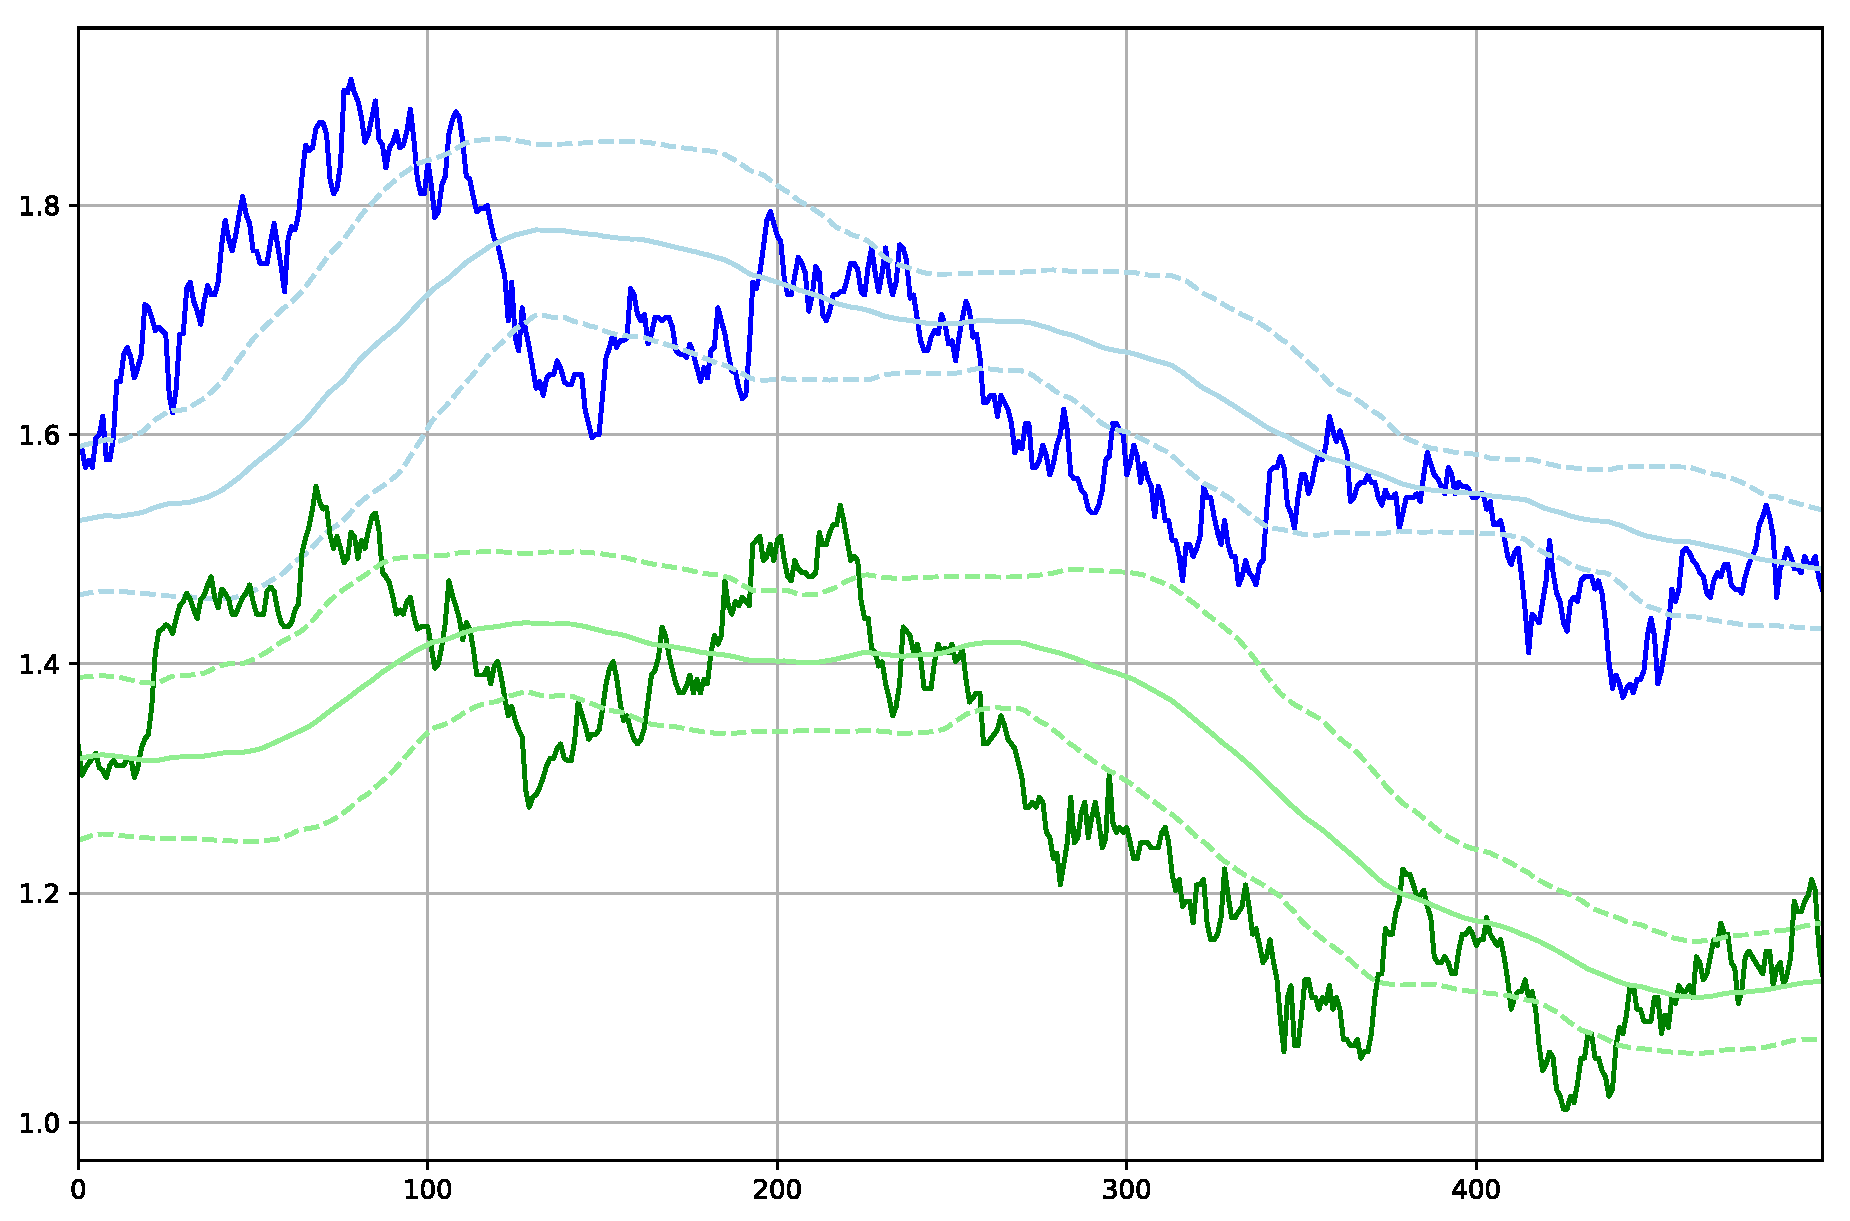
\includegraphics[width=1.0\linewidth]{graphics/ab-prices.pdf}
    \caption{
      Prikaz kretanja cijena dviju vrijednosnica, $X$ i $Y$, u razdoblju od 500 dana.
      Plavom bojom prikazana je cijena $P_X^{(t)}$, a zelenom cijena $P_Y^{(t)}$.
      Svjetlijim nijansama tih boja prikazano je punom linijom očekivanje, i crtkanom linijom udaljenost za jednu devijaciju od očekivanja; očekivanje i devijacija izračunati su u svakom trenutku na proteklom periodu $T$ duljine 120 dana.
    }
    \label{fig:ab-prices}
  \end{figure}

  \begin{figure}[p]
    \centering
    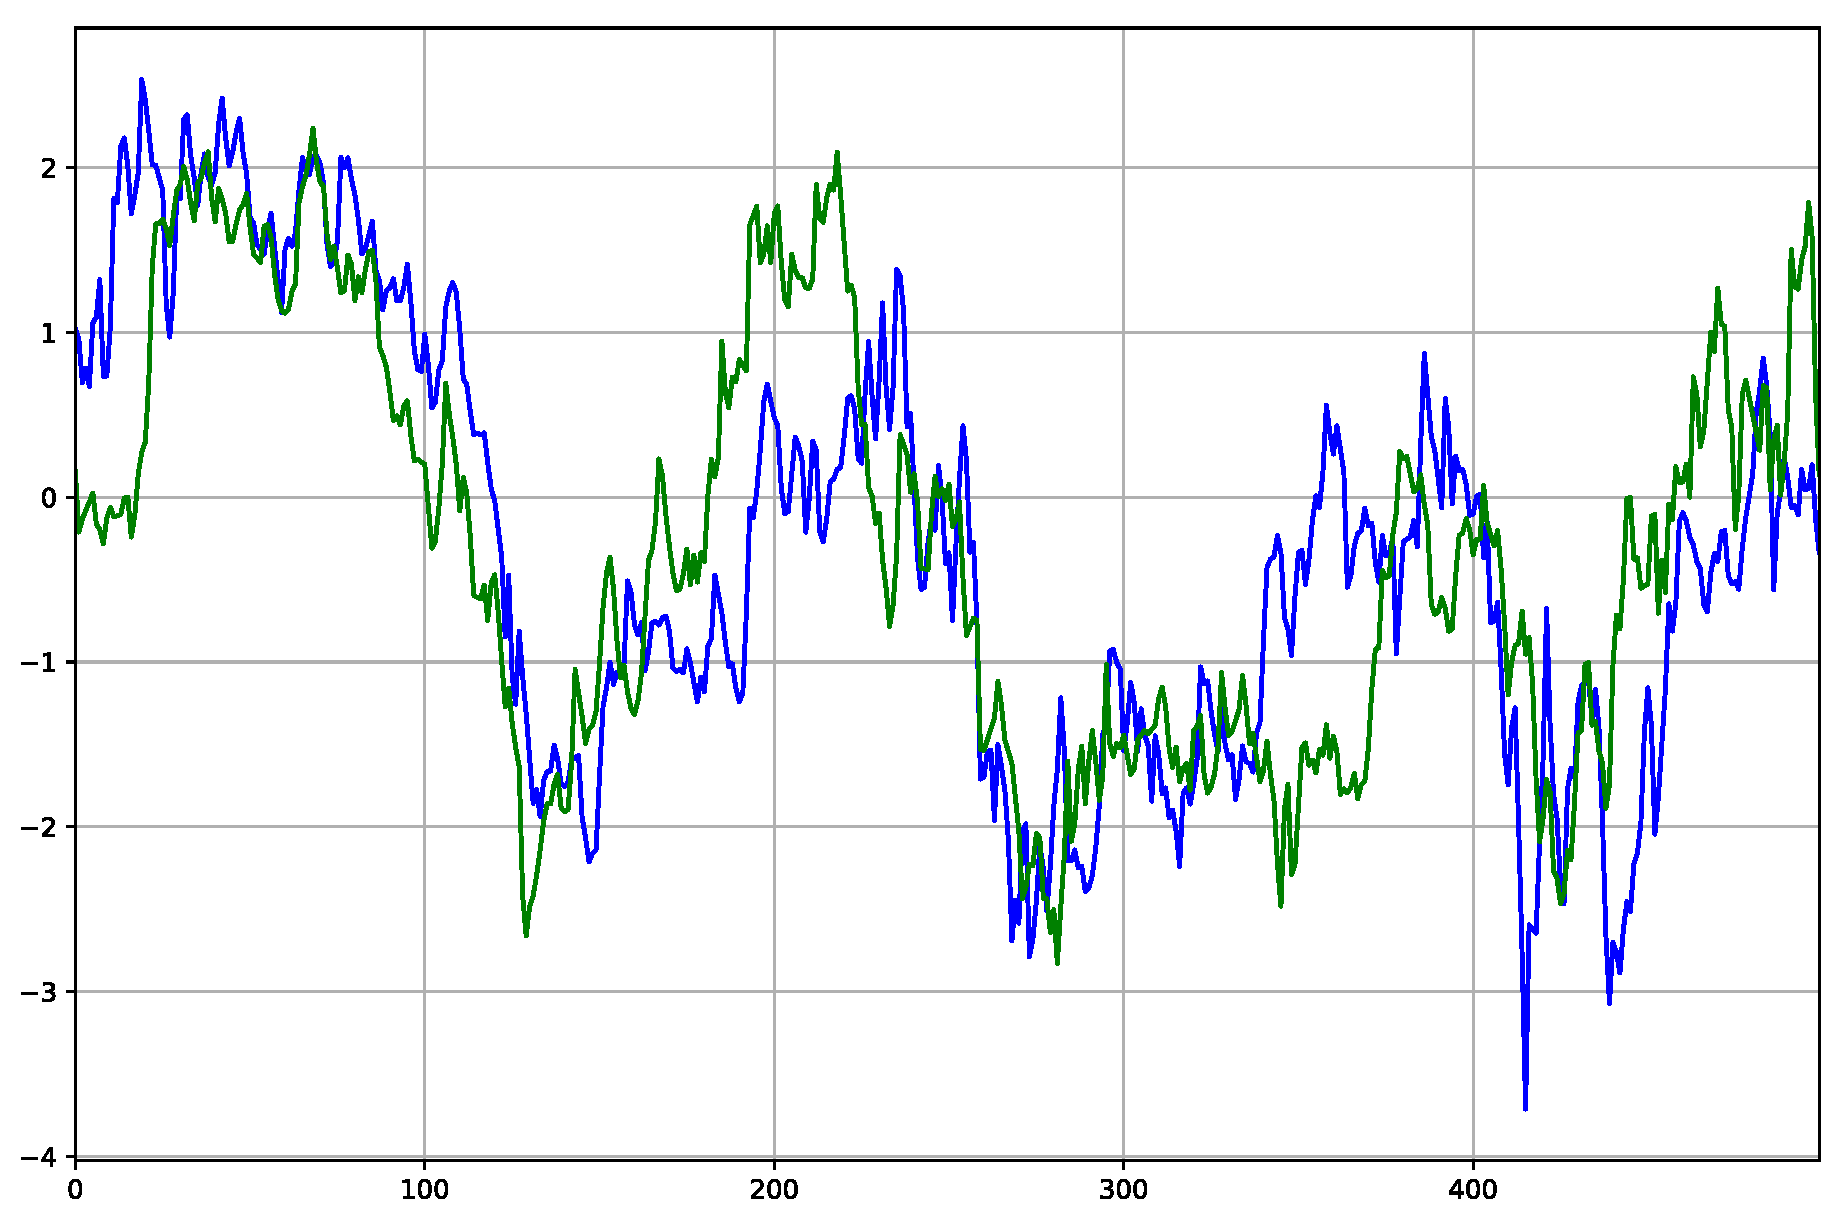
\includegraphics[width=1.0\linewidth]{graphics/ab-prices-norm.pdf}
    \caption{
      Plavo: normalizirana cijena $\norm{P}_X^{(t)}$, zeleno: normalizirana cijena $\norm{P}_Y^{(t)}$.
    }
    \label{fig:ab-prices-norm}
  \end{figure}

  \begin{figure}[p]
    \centering
    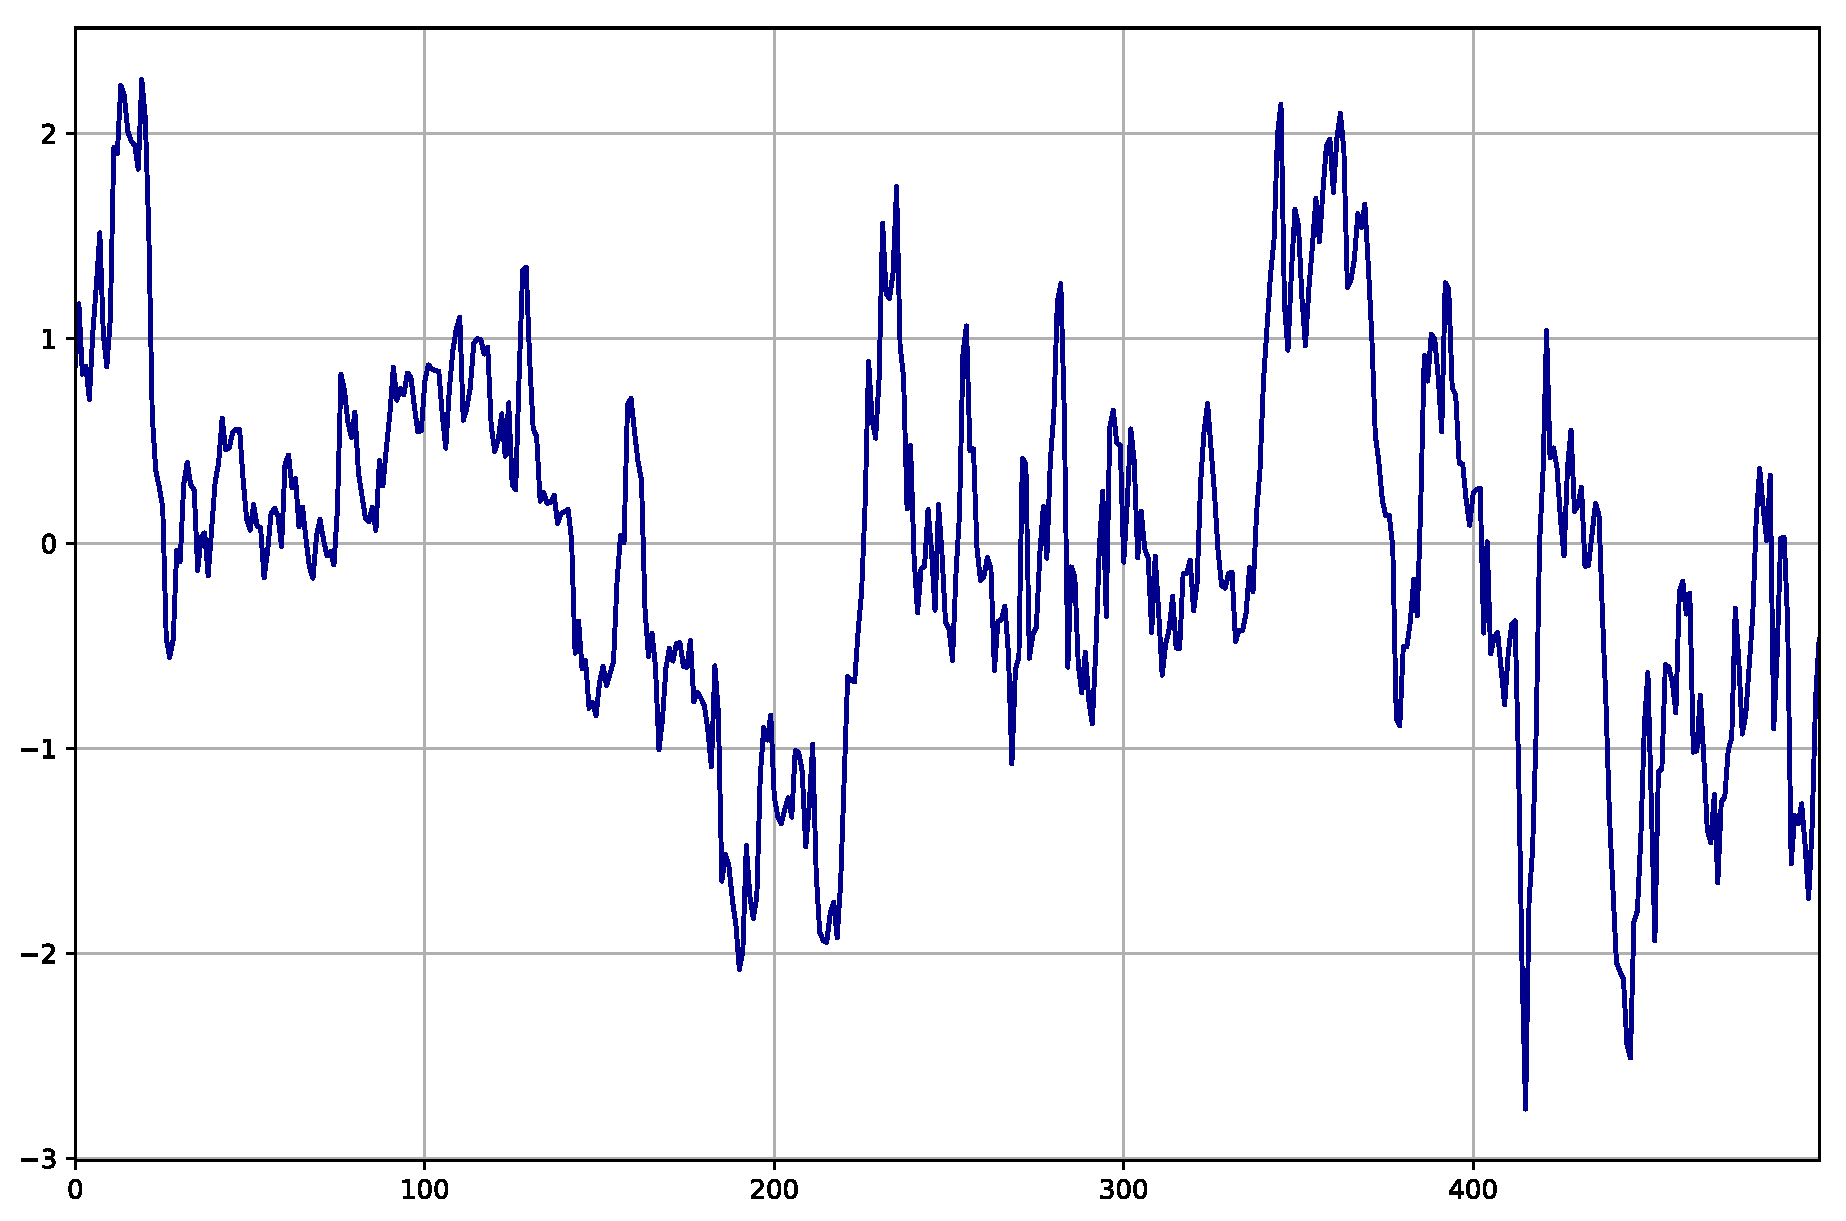
\includegraphics[width=1.0\linewidth]{graphics/ab-prices-norm-diff.pdf}
    \caption{
      Razlika normaliziranih cijena, $D_{X,Y}^{\q(t\w)}$.}
    \label{fig:ab-prices-norm-diff}
  \end{figure}
  
  \subsection{Normalizirana razlika log-cijena}
  Za razliku od prethodne mjere sličnosti, u ovom slučaju razlika se računa nad nenormaliziranim log-cijenama za sve $t$, označeno s $d_{X,Y}^{\q(t\w)}$:
  \begin{equation}
  d_{X,Y}^{\q(t\w)} = P_X^{\q(t\w)} - P_Y^{\q(t\w)},
  \end{equation}
  a zatim se iz razlika $d_{X,Y}^{\q(t\w)}$ računaju normalizirane razlike $\norm{d}_{X,Y}^{\q(t\w)}$ za $t \ge T$:
  \begin{equation}
  \norm{d}_{X,Y}^{\q(t\w)} = \frac{d_{X,Y}^{\q(t\w)} - \Efromto{d_{X,Y}^{(\tau)}}{t-T \le \tau < t}}{\sqrt{\Varfromto{d_{X,Y}^{(\tau)}}{t-T \le \tau < t}}}.
  \end{equation}
  Ovako dobivena normalizirana razlika log-cijena koristi se kao mjera sličnosti.
  U odnosu na prethodnu, ova mjera je više osjetljiva na promjene log-cijena neovisno o volatilnostima samih vrijednosnica, što će doći do izražaja prilikom usporedbe dviju vrijednosnica čije se cijene mijenjaju različitom brzinom i intenzitetom.
  Primjer razlike nenormaliziranih log-cijena istih dionica $X$ i $Y$, kao i u prethodnom slučaju, prikazan je na slici \ref{fig:diff}, te normalizirane razlike na slici \ref{fig:diff-norm}.
  
  \begin{figure}[H]
    \centering
    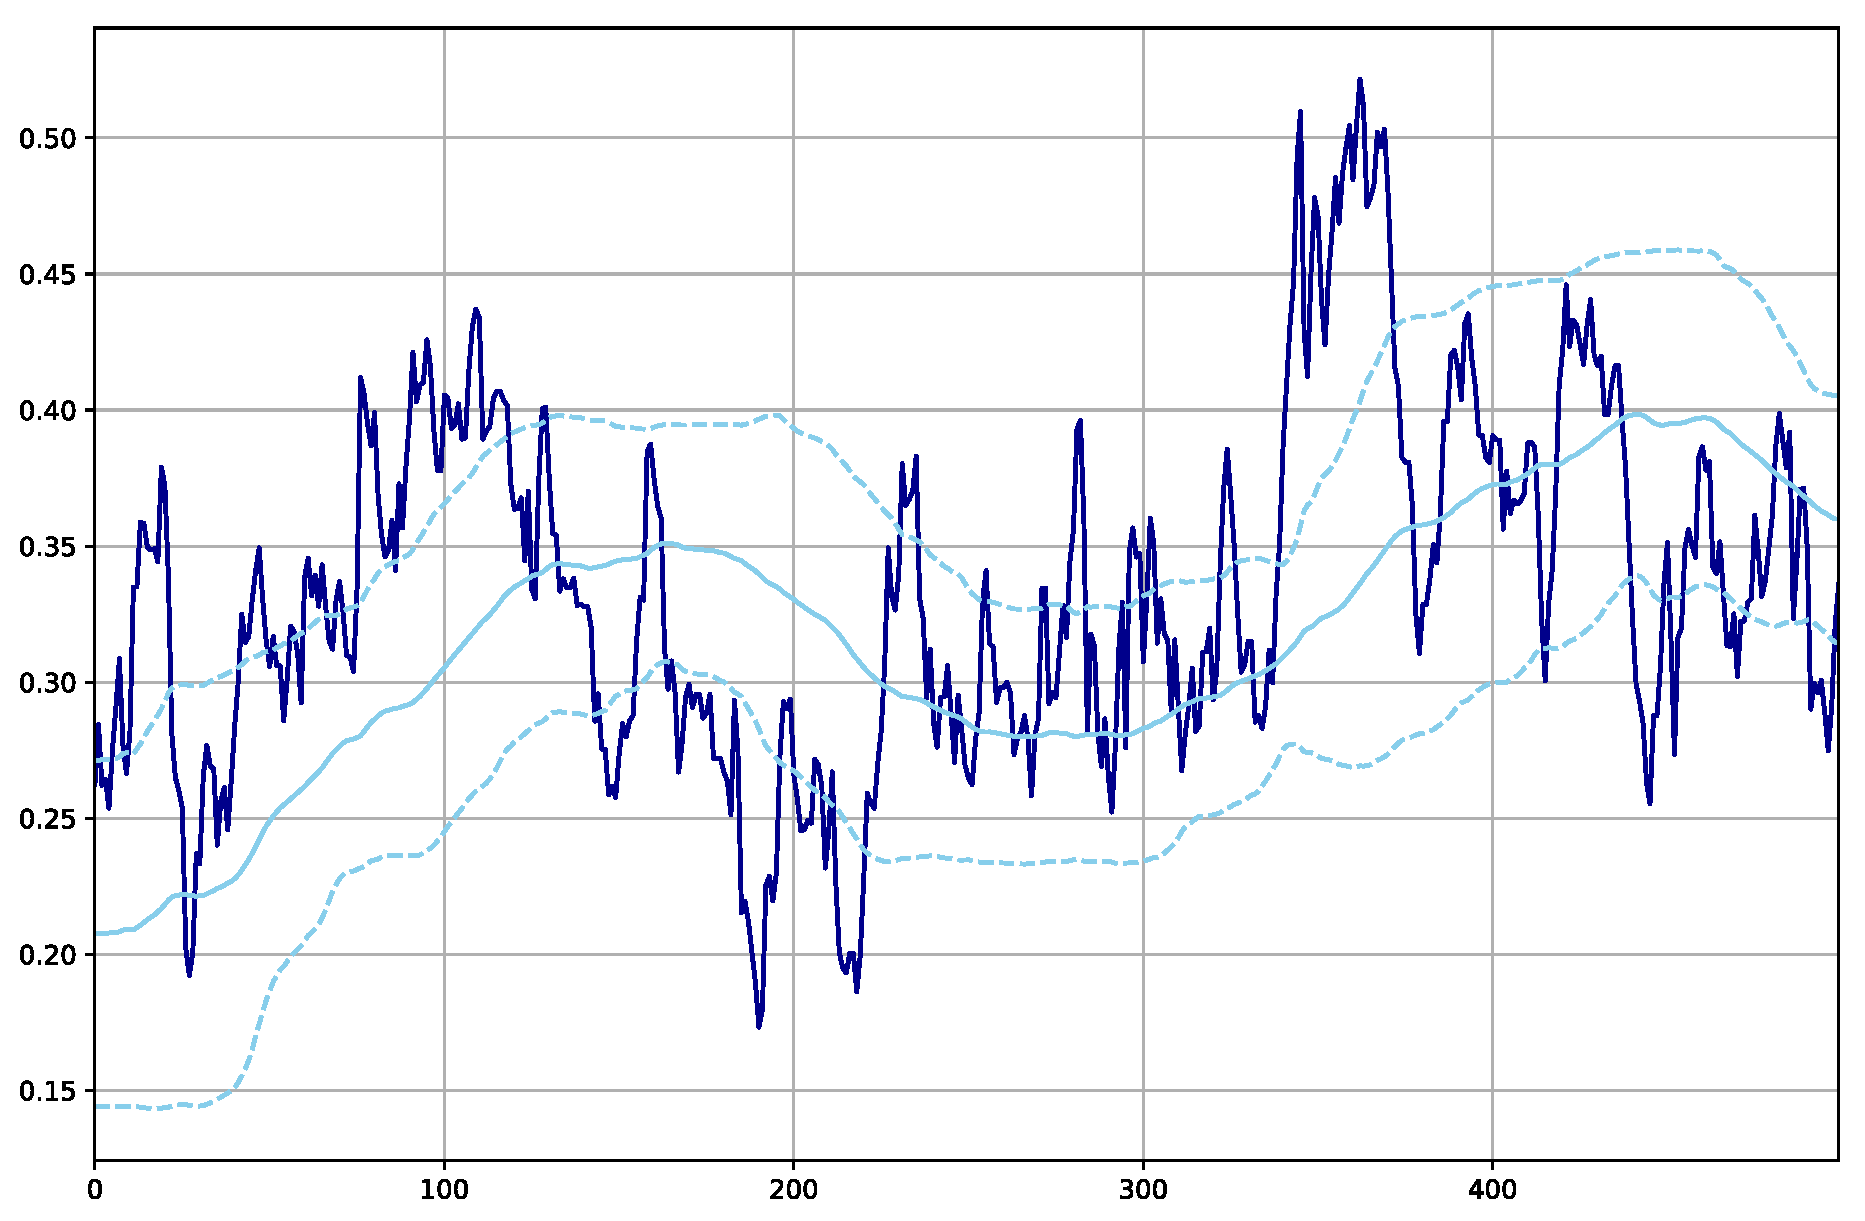
\includegraphics[width=1.0\linewidth]{graphics/diff.pdf}
    \caption{Tamnijom bojom prikazana je razlika nenormaliziranih cijena $d_{X,Y}^{(t)}$, a svjetlijom punom linijom očekivanje i crtkanom linijom udaljenost od očekivanja za jednu devijaciju.}
    \label{fig:diff}
  \end{figure}

  \begin{figure}[H]
    \centering
    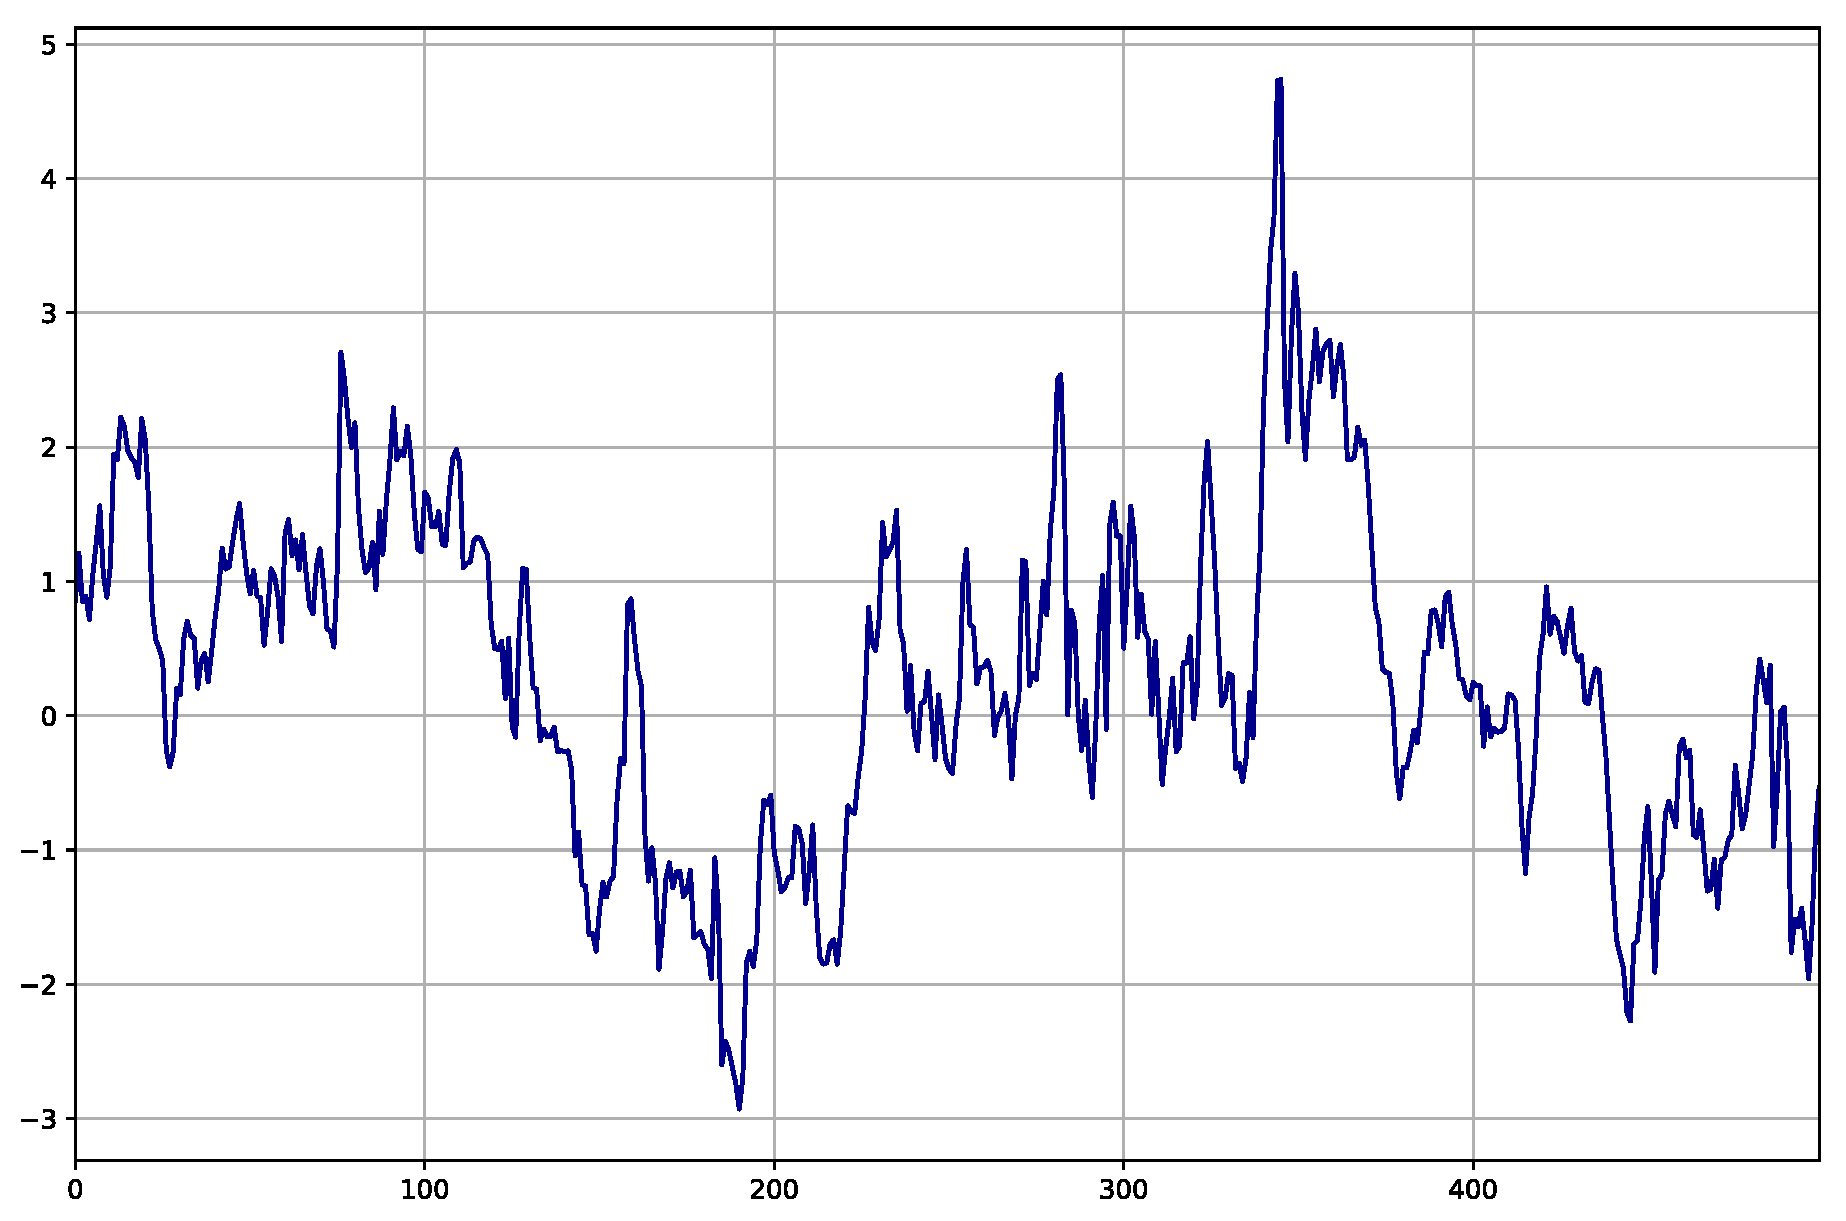
\includegraphics[width=1.0\linewidth]{graphics/diff-norm.pdf}
    \caption{
      Normalizirana razlika cijena, $\norm{d}_{X,Y}^{\q(t\w)}$.}
    \label{fig:diff-norm}
  \end{figure}
  
  \subsection{Mjera kointegracije slučajnih procesa}
  Za razliku od prethodne dvije mjere sličnosti gdje se cijene dionica tretiraju kao vremenski nizovi, kod ove mjere one se tretiraju kao realizacije diskretnog slučajnog procesa.
  Za neki slučajni proces zanimljivo je proučiti svojstvo stacionarnosti --- slučajni proces $U\q[t\w]$ je stacionaran ako i samo ako vrijedi:
  \begin{gather}
  \label{eq:stat1}
  \E{U\q[t\w]} = \mathrm{const.}\\
  \label{eq:stat2}
  \R{UU}{t, \tau} = \E{U\q[t\w] \cdot U\q[t + \tau\w]} = \R{UU}{\tau}.
  \end{gather}
  Za stacionarne slučajne procese vrijedi da njihova statistička svojstva ne ovise o vremenu:
  jednadžba (\ref{eq:stat1}) tvrdi da je za stacionaran proces $U\q[t\w]$ očekivanje $\E{U\q[t\w]}$ neovisno o vremenu $t$, a jednadžba (\ref{eq:stat2}) tvrdi da njegova autokorelacija $\R{UU}{t, \tau}$ ovisi samo o vremenskom pomaku $\tau$, ali ne i o $t$.
  Ovakva definicija stacionarnosti naziva se još i ``stacionarnost u širem smislu''.
  
  Red integracije slučajnog procesa, označen s $\I{d}$, gdje je $d$ red integracije, opisuje njegovu stacionarnost.
  Stacionarni slučajni procesi su $\I{0}$.
  Za općenit proces $V\q[t\w]$ koji je $\I{1}$ vrijedi da je proces $\diff V\q[t\w]$ dobiven njegovim diferenciranjem
  \begin{equation}
  \label{eq:red1}
  \diff V\q[t\w] = \q(1 - \lag\w) V\q[t\w] = V\q[t\w] - V\q[t - 1\w]
  \end{equation}
  stacionaran proces, a za općenit proces $W\q[t\w]$ koji je $\I{d}$ vrijedi da je proces $\diffn{d} W\q[d\w]$ dobiven njegovim uzastopnim diferenciranjem $d$ puta
  \begin{align}
  \diffn{d} W\q[t\w] &= \q(1 - \lag\w)^d W\q[t\w] = \q( \sum_{n = 0}^{d} \binom{d}{n} \q(-1\w)^n\lag^n \w) W\q[t\w] \nonumber \\
  \label{eq:redn}
  &= \sum_{n = 0}^{d} \binom{d}{n} \q(-1\w)^n W\q[t - n\w]
  \end{align}
  stacionaran proces.
  U (\ref{eq:red1}) i (\ref{eq:redn}) korišten je operator kašnjenja $\lag$ koji djeluje na sljedeći način: $\lag \q\{U\q[t\w]\w\} = U\q[t - 1\w]$.
  
  Trivijalno je provjeriti da linearna kombinacija dvaju slučajnih procesa koji su $\I{0}$ jest također $\I{0}$, kao i da linearna kombinacija dvaju slučajnih procesa od kojih je jedan $\I{0}$, a drugi $\I{1}$ jest $\I{1}$.
  Malo je teže odrediti kojeg je reda integracije linearna kombinacija dvaju slučajnih procesa koji su $\I{1}$: to može biti $\I{1}$, ali u posebnim slučajevima može biti i $\I{0}$.
  Kointegracija dvaju slučajnih procesa $X\q[t\w]$ i $Y\q[t\w]$ koji su $\I{1}$ označava da je njihova linearna kombinacija $U\q[t\w]$ stacionaran proces, odnosno $\I{0}$:
  \begin{equation}
  X\q[t\w] + \beta Y\q[t\w] = U\q[t\w],
  \end{equation}
  gdje je $\beta$ konstanta koja se još naziva i kointegracijski koeficijent.
  Stacionarni slučajni proces $U\q[t\w]$ pritom se može prikazati kao:
  \begin{equation}
  U\q[t\w] = \mu + \varepsilon\q[t\w],
  \end{equation}
  gdje je $\mu = \E{U\q[t\w]}$, očekivanje, a $\varepsilon\q[t\w]$ rezidualna vrijednost za koju vrijedi $\E{\varepsilon\q[t\w]} = 0$.
  
  Pretpostavka kod ove mjere sličnosti jest da su dva nestacionarna slučajna procesa $P_X\q[t\w]$ i $P_Y\q[t\w]$ koji predstavljaju kretanje log-cijena vrijednosnica $X$ i $Y$ kointegirana.
  Postoji nekoliko metoda za provjeru kointegracije, najčešće korištene su Engle-Granger metoda, Johansen metoda i Phillips-Ouliaris metoda.
  Najjednostavnija od navedenih je Engle-Granger metoda, koja je opisana u nastavku.
  
  Ideja metode Engle-Granger je u prvom koraku estimirati stacionaran proces $U\q[t\w]$ koji je linearna kombinacija cijena $P_X\q[t\w]$ i $P_Y\q[t\w]$, zatim u drugom koraku provjeriti je li estimirani proces zaista stacionaran \citep{engle-granger}.
  Postupkom najmanjih kvadrata najprije se određuju procjene parametara $\mu$ i $\beta$, označene s $\hat{\mu}$ i $\hat{\beta}$:
  \begin{equation}
  \hat{\mu}, \hat{\beta} = \argmin_{\mu, \beta} \q\{\sum_{\tau = t - T}^{t - 1} \q \lvert P_X\q[\tau\w] + \beta P_Y\q[\tau\w] -\mu \w \rvert^2\w\},
  \end{equation}
  a zatim se izraze procijenjene rezidualne vrijednosti $\hat{\varepsilon}\q[t\w]$:
  \begin{equation}
  \hat{\varepsilon}\q[t\w] = -\hat{\mu} + P_X\q[t\w] + \hat{\beta} P_Y\q[t\w].
  \end{equation}
  
  U drugom koraku provjerava se je li $\hat{\varepsilon}\q[t\w]$ zaista stacionaran proces: za dobivenu procjenu statističkim metodama računaju se $t$-vrijednosti kako bi se utvrdila pouzdanost kointegracije.
  $t$-vrijednost može se dobiti Dickey-Fullerovim testom \citep{dickey-fuller}.
  
  Procijenjene rezidualne vrijednosti $\hat{\varepsilon}\q[t\w]$ koriste se kao mjera sličnosti.
  Primjer dobivenih rezidualnih vrijednosti za iste vrijednosnice $X$ i $Y$ prikazan je na slici \ref{fig:residual}.
  U odnosu na prethodne dvije mjere, ova mjera je rezultat dublje statističke analize, zbog čega je i računski zahtjevnija, što je ujedno i prednost i nedostatak.
  Kada se radi o velikom broju parova vrijednosnica, mjera kointegracije može se pokazati nepraktičnom za računanje, stoga je bolje koristiti neku od dvije prethodno navedene mjere sličnosti.
  U ovom radu korištena je normalizirana razlika log-cijena.
  
  \begin{figure}[H]
    \centering
    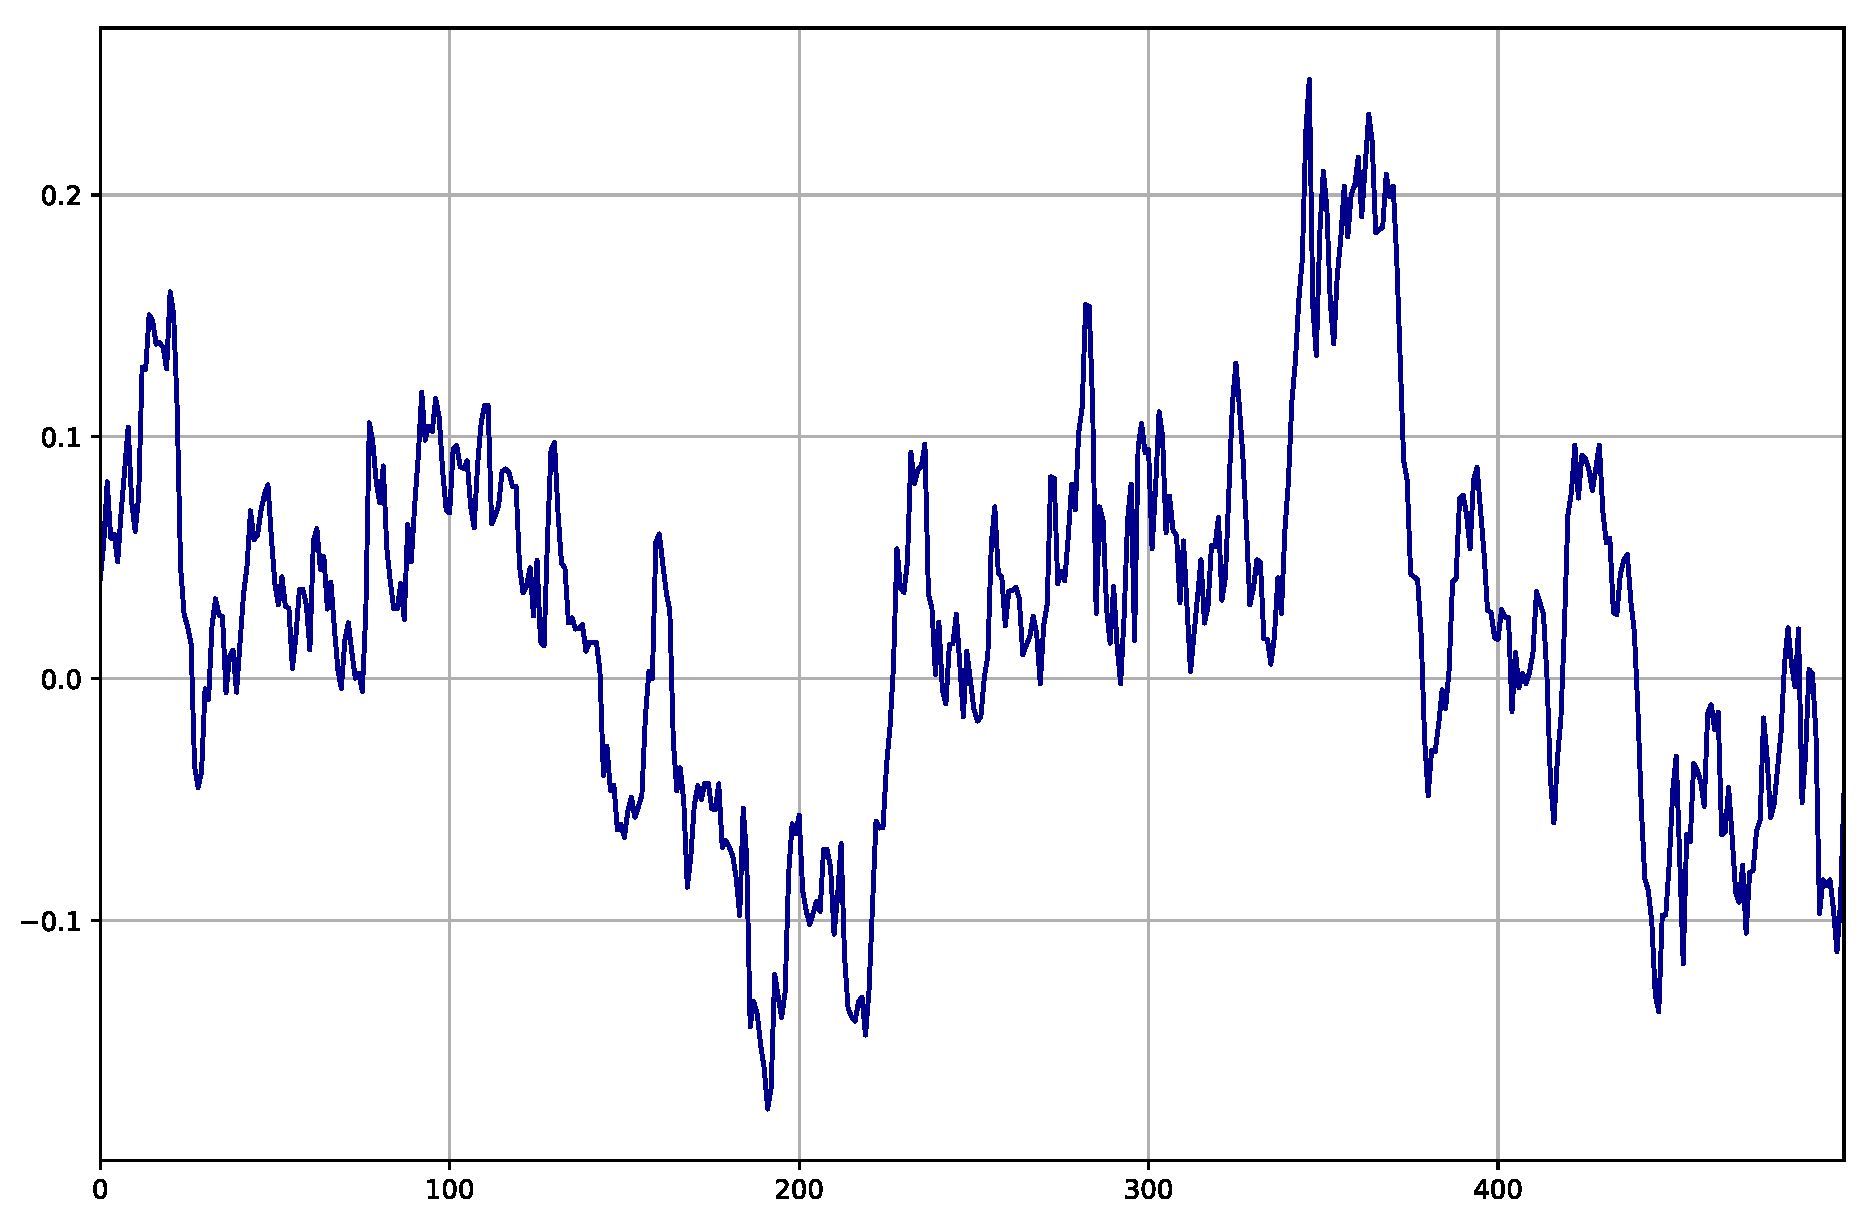
\includegraphics[width=1.0\linewidth]{graphics/residual.pdf}
    \caption{
      Procijenjene rezidualne vrijednosti $\hat{\varepsilon}\q[t\w]$ u slučaju vrijednosnica $X$ i $Y$.}
    \label{fig:residual}
  \end{figure}
  
  \subsection{Nedostaci statističke arbitraže}
  Jedan od nedostataka statističke arbitraže jest relativno niska točnost u predviđanju kretanja cijene, ako se odluke o trgovanju promatraju kao klasifikacijski problem predviđanja rasta ili pada cijene vrijednosnice.
  Točnost $\mathit{Acc}$ računa se kao:
  \begin{equation}
    \mathit{Acc} = \frac{\mathit{TP} + \mathit{TN}}{\mathit{TP} + \mathit{FP} + \mathit{FN} + \mathit{TN}},
  \end{equation}
  gdje su $\mathit{TP}$ \engl{true positive}, $\mathit{FP}$ \engl{false positive}, $\mathit{FN}$ \engl{false negative}, i $\mathit{TN}$ \engl{true negative} odgovarajući brojevi pogođenih ili promašenih predviđanja pada ili rasta cijene kako je opisano na slici \ref{fig:confusion_matrix}.
  \begin{figure}[h]
    \centering
    \renewcommand{\arraystretch}{1.4}
    \begin{tabular}{>{\centering}m{-1em} >{\centering}m{-1em} >{\centering}m{0.6em} >{\centering}m{2em}>{\centering\arraybackslash}m{2em}}
      & & & \multicolumn{2}{c}{ostvareno} \\[-1.8em]
      & & & \multicolumn{2}{c}{\downbracefill} \\[-1.8em]
      & & & raste & pada \\[-0.4em] \cline{4-5}
      \parbox[s]{2mm}{\multirow{2}{*}{\rotatebox[origin=c]{90}{predviđeno\hspace{0.5em}}}} & \ldelim\{{2.2}{1mm} & 
      \parbox[s]{2mm}{\rotatebox[origin=c]{90}{\small raste}} & \multicolumn{1}{|c|}{\textbf{TP}} & \multicolumn{1}{c|}{\textbf{FP}} \\ \cline{4-5}
      & & \parbox[s]{2mm}{\rotatebox[origin=c]{90}{\small pada}} & \multicolumn{1}{|c|}{\textbf{FN}} & \multicolumn{1}{c|}{\textbf{TN}} \\ \cline{4-5}         
    \end{tabular}
    \renewcommand{\arraystretch}{1}
    \caption{Moguće kombinacije predviđenih i ostvarenih kretanja cijene.}
    \label{fig:confusion_matrix}
  \end{figure}
  Može se pretpostaviti da je broj trgovanja u kojima cijena stvarno raste i pada podjednak.
  Pri testiranju algoritma statističke arbitraže nad testnim skupovima podataka točnost rijetko kada prelazi 60\%, a najčešće je manja od 50\%.
  Jedan od razloga slabe točnosti predviđanja je činjenica da je samo kretanje cijena slučajan proces čije je ponašanje teško predvidjeti.
  Korištene metode u algoritmu pokušavaju na temelju statističkih zakonitosti utvrditi vjerojatnosti kretanja cijena.
  Također, uzrok može biti i prividna korelacija \engl{spurious correlation} u kojoj kretanje cijena dviju vrijednosnica izgleda povezano, no zapravo je uzrok tome neki nepoznati vanjski faktor.
  Prividna korelacija na tržištima opisana je u \citep{spurious}.
  Na primjer, ako se dogodi da na tržištu istovremeno raste potražnja za sladoledom i rashladnim uređajima, moglo bi se zaključiti kako postoji povezanost među njima, ali je vjerojatnije povećanje potražnje uzrokovao faktor koji nije bio uzet u obzir, primjerice visoka temperatura.
  Tada predviđeno ponašanje može biti poprilično različito od ostvarenog, budući da vanjski faktor može prestati utjecati u bilo kojem trenutku, a time se i gubi prividna korelacija.
  Isto tako, statističke metode ne mogu razlikovati prirodne devijacije u ponašanju cijena koje su karakteristične za slučajne procese, od onih prisilnih za koje stvarno postoji fundamentalan uzrok, kao što je npr. značajna promjena u načinu poslovanja neke firme, promjena vlasništva i tome slično.
  No, unatoč tome što algoritam griješi u više od pola slučajeva, ukupni profit je ipak pozitivan, jer pogreške donose znatno manje gubitke u odnosu na zaradu ostvarenu pogocima.
  
  Drugi nedostatak tiče se načina na koji se raspoložive vrijednosnice uzimaju u obzir.
  Svaki par vrijednosnica gleda se zasebno i pritom je isključena dublja analiza međusobnih interakcija svih vrijednosnica zajedno.
  Trgovanje se također odvija uvijek u parovima, zauzimanjem kratke pozicije u jednoj i duge u drugoj, što zahtijeva da je kratka pozicija dopuštena na tržištu, a to ne mora biti slučaj.
  Također, pokazalo se da ovaj način promatranja parova zasebno rezultira jako visokim koeficijentom obrtaja\footnote{Koeficijent obrtaja opisan je u odjeljku \ref{sc:turnover}.}, odnosno portfelj dobiven isključivo metodom statističke arbitraže je vrlo promjenljiv.
  Češće mijenjanje vrijednosnica u portfelju uzrokuje i veće troškove trgovanja, što u konačnici smanjuje i ukupnu vrijednost portfelja.
  U ovom radu istražena je metoda koja omogućuje trgovanje kupovanjem i prodajom svih vrijednosnica neovisno o parovima, koristeći pritom metode statističke arbitraže za opisivanje relacije preferencije među vrijednosnicama.
  Interakcija među vrijednosnicama opisuje se grafom toka preferencija, iz čega se naposljetku izvlači poredak prema individualnoj preferenciji svih vrijednosnica.
  
%  Nedostaci klasičnih metoda statističke arbitraže su: faljivanje. Kad se uključe troškovi trgovanja...
%  Tretiranje parova dionica zasebno, nedostaje interakcija između svih dionica zajedno.

  \section{Relacija preferencije i funkcija korisnosti}
%  Let $\Omega$ be any set of entities.
  Neka je $\Omega$ skup općenitih dobara.
%  Preference relation $\succ$ defined over $\Omega \times \Omega$ is a strict weak ordering that describes the way humans prefer some entity over another.
  Relacija preferencije, označena simbolom $\succ$ i definirana nad $\Omega \times \Omega$, je strogi slabi uređaj koji odgovara načinu na koji ljudi preferiraju jednu vrijednosnicu u odnosu na drugu.
  Između dvaju dobara $a, b \in \Omega$ relacija može, ali i ne mora postojati.
  Primjerice, $a$ može biti više preferirano u odnosu na $b$, ili $b$ u odnosu na $a$, ali moguća je situacija gdje su oba dobra podjednako preferirana.
  U tom slučaju radi se o indiferentnosti između $a$ i $b$, što se označava kao $a \sim b$.
%  This relation is specific in that it is ($\forall x, y, z \in \Omega$):

  Ova relacija specifična je po tome što je:
  \begin{itemize}
%    \item \textit{irreflexive}: every entity $x$ is not preferrable over itself, %($\neg \q( x \succ x \w)$),
    \item \textit{irefleksivna}: $\forall x \in \Omega\colon \neg \q( x \succ x \w)$ --- ni za jedno dobro ne vrijedi da je više preferirano od samog sebe,
%    \item \textit{asymmetrical}: if $x$ is preferrable over some $y$, then $y$ is not preferrable over $x$, %($x \succ y \Rightarrow \neg \q( y \succ x \w)$),
    \item \textit{asimetrična}: $\forall x, y \in \Omega\colon x \succ y \Rightarrow \neg \q( y \succ x \w)$ --- ako je $x$ više preferirano od $y$, onda $y$ nije više preferirano od $x$,
%    \item \textit{transitive}: if $x$ is preferrable over $y$, and $y$ is preferrable over $z$, then $x$ is also preferrable over $z$, %($x \succ y \wedge y \succ z \Rightarrow x \succ z$),
    \item \textit{tranzitivna}: $\forall x, y, z \in \Omega\colon x \succ y \wedge y \succ z \Rightarrow x \succ z$ --- ako je $x$ više preferirano od $y$, i $y$ više preferirano od $z$, tada je i $x$ više preferirano od $z$,
%    \item \textit{transitive in incomparability} (noting that $x$ and $y$ may be \textit{incomparable}, i.e. neither $x$ is preferrable over $y$, nor $y$ is preferrable over $x$): if $x$ is incomparable with $y$, and $y$ is incomparable with $z$, then $x$ is also incomparable with $z$.
    \item \textit{tranzitivna po indiferentnosti}: $\forall x, y, z \in \Omega\colon x \sim y \wedge y \sim z \Rightarrow x \sim z$ --- ako je $x$ podjednako preferirano kao i $y$, i $y$ podjednako preferirano kao i $z$, tada je i $x$ podjednako preferirano kao i $z$.
  \end{itemize}
  
%  We naturally assume this kind of relation we describe relationships among the assets.
%  Determining that some asset is preferred over another is easier than assigning a preference rank to each asset individually, especially for a larger number of assets.
%  However, the latter is more useful for decision making, and therefore it is desirable to find a way of sorting assets in the order of preference.
  Relacija preferencije koristi se u mikroekonomici u svrhu vrednovanja međusobnog odnosa različitih dobara \citep{inzeko}.
  Ovakva vrsta relacije prirodno opisuje odnose među različitim vrijednosnicama, npr. dionica $A$ u nekom trenutku može biti više preferirana od dionice $B$.
  Razlog tome je što je za čovjeka lakše ocijeniti odnos (više, manje, jednako preferirano) između svakog para vrijednosnica, nego pridijeliti svakoj vrijednosnici individualnu mjeru preferencije, pogotovo ako se radi o velikom broju vrijednosnica.
  No ipak, u svrhu konstruiranja portfelja korisnije je posjedovati individualnu mjeru preferencije za svaku vrijednosnicu.
  Stoga je poželjno pronaći način da se iz relacije preferencije dobiju individualne mjere preferencije.
  
%  Utility function $U\colon \Omega \to \mathbb{R}$ is mapping from entities to real numbers, in such way that order of the mapping corresponds to the preference order of the entities, i.e. $\forall x, y \in \Omega, U(x) > U(y) \Rightarrow x \succ y$.
%  One such mapping is obtained by using potential method that is described later in this paper.
%  In addition to ordering of the entities, utility function also provides the intensity of preference for a particular entity, hence it is more informative when it comes to the decision making.
  Funkcija korisnosti \engl{utility function} $U\colon \Omega \to \mathbb{R}$ je preslikavanje iz skupa dobara u skup realnih brojeva, na način da poredak preslikanih realnih brojeva odgovara poretku dobara prema individualnoj preferenciji, tj. vrijedi:
  \begin{equation*}
    \forall x, y \in \Omega \colon x \succ y \Leftrightarrow U\q(x\w) > U\q(y\w).
  \end{equation*}
  Posljedično, za indiferentnost vrijedi:
  \begin{equation*}
    \forall x, y \in \Omega \colon x \sim y \Leftrightarrow U\q(x\w) = U\q(y\w).
  \end{equation*}
  Jedno takvo preslikavanje ostvaruje se korištenjem metode potencijala koja je opisana u poglavlju \ref{sec:metpot}.
  Ekvivalencija metode potencijala i funkcije korisnosti pokazana je u radu \citep{metpotexact}.
  Osim što određuje poredak dobara prema individualnoj preferenciji, funkcija korisnosti također kvantificira preferenciju time što unosi intenzitet preferencije jedne vrijednosnice u odnosu na drugu; stoga funkcija korisnosti nosi više informacija od same relacije.

  \section{Graf toka preferencija}
  Graf toka preferencija je pomoćna struktura koja služi pri prevođenju toka preferencija među čvorovima u individualne mjere preferencije svakog čvora.
  U odnosu na relaciju preferencije koja je implicirana njime, graf sadrži još i intenzitete preferencija jednih čvorova nad drugima.
  Ako se zanemare težine bridova u grafu i ostave samo smjerovi, iz njega se direktno može pročitati relacija preferencije koju on opisuje.
  Težine u grafu daju dodatnu informaciju o individualnim mjerama preferencije čvorova koje odgovaraju toj relaciji preferencije, za razliku od situacije kada težina nema, što je ekvivalentno tome da su sve preferencije jednakog intenziteta.
  U odnosu na individualne mjere preferencije svakog čvora zasebno, graf toka preferencija ne određuje poredak čvorova prema preferenciji.
  
  
%  Graph of preference flow is a weighted directed graph without multiple edges and loops, whose nodes represent entities, edges represent preference for one entity over another, and edge weights correspond to the strength of the preferences.
%  If an edge between nodes is missing, it is considered that neither entity is preferable over another (incomparability of entities).
%  The graph as a whole describes preference flow among the entities.
%  An example of graph is shown on Fig. \ref{fig:graph}.
  Graf toka preferencija je težinski usmjereni graf, bez višestrukih bridova i petlji (bridova koji počinju i završavaju u istom grafu).
  Njegovi čvorovi predstavljaju vrijednosnice, usmjereni bridovi preferenciju jedne vrijednosnice nad drugom, a težine bridova odgovaraju intenzitetu preferencije.
  Ako između dva čvora nedostaje brid, smatra se da su pripadne vrijednosnice podjednako preferirane (indiferentnost u odlučivanju kod relacije preferencije).
  Graf kao cjelina opisuje tok preferencija među vrijednosnicama.
  Primjer grafa toka preferencija prikazan je na slici \ref{fig:graph}.
  
  \begin{figure}[h]
    \centering
    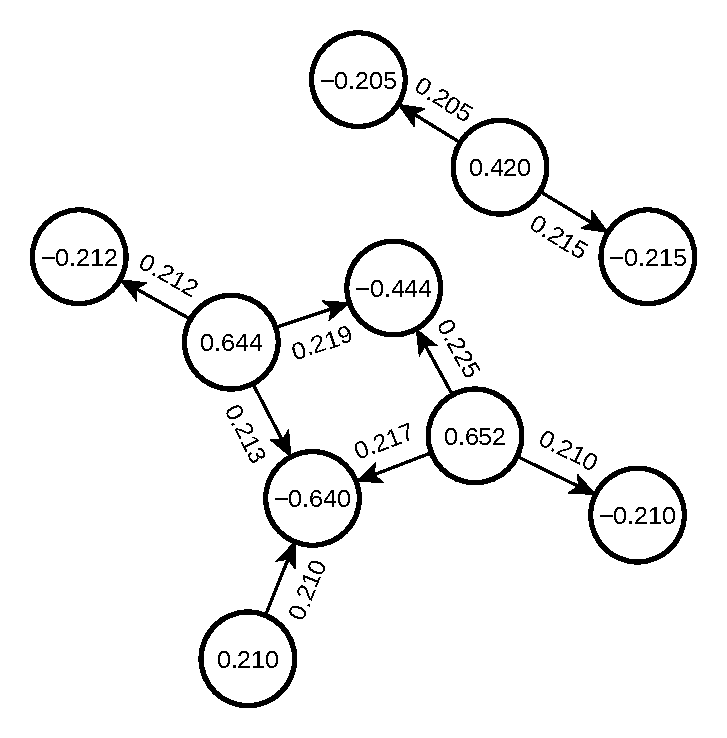
\includegraphics[width=0.65\columnwidth]{graphics/pref-flow-graph.pdf}
    \caption{Primjer grafa toka preferencija. Na bridovima su prikazani intenziteti preferencija jedne vrijednosnice u odnosu na drugu, a u čvorove su upisane individualne mjere preferencija za pripadni čvor izračunate kao razlika zbroja težina bridova koji izlaze iz tog čvora i zbroja težina bridova koji ulaze u taj čvor. Opravdanje za takav postupak dano je u odjeljku \ref{sec:metpot}. Ovaj graf je konzistentan s relacijom preferencije koju predstavlja.}
    \label{fig:graph}
  \end{figure}
  
%  Construction of the graph is based on a statistical arbitrage method.
%  An edge going from node $i$ to node $j$ with weight $w_{i,j}$ will be present in the graph if and only if assets represented by nodes $i$ and $j$ have demonstrated similar behavior during the past period, but have suddenly diverged at the moment, as determined per statistical measures.
%  Weight $w_{i,j}$ corresponds to the magnitude of this divergence.  
%  A detailed description of used statistical measures the procedure is given later in \ref{sub:creating-graph}.
  
  Konstrukcija grafa u ovom radu temelji se na metodi statističke arbitraže.
  Brid koji ide od čvora $i$ do čvora $j$ s težinom $w_{i,j}$ je prisutan u grafu ako i samo ako su se dvije pripadne vrijednosnice $i$ i $j$ ponašale slično tijekom proteklog perioda, ali su se prema određenim statističkim mjerama trenutačno razdvojile.
  Težina $w_{i,j}$ opisuje intenzitet ovog razdvajanja i služi kao mjera intenziteta preferencije jedne vrijednosnice u odnosu na drugu.
  Podrazumijeva se da je $w_{i,j} = -w_{j,i}$, odnosno negativan intenzitet preferencije označava da je jedna vrijednosnica toliko manje preferirana u odnosu na drugu.
  Detaljan opis postupka dobivanja korištenih statističkih mjera dan je u odjeljku \ref{sub:creating-graph}.
    
%  Connections in this graph impose a preference relation among entities that are presented by the graph, in the way that an edge that goes from node $A$ to node $B$ means that $A$ is preferred over $B$.
%  It is the case that neither node is in relation with itself (irreflexivity), and that no multiple connections are allowed between two nodes (implies asymmetry).
%  However, problems arise with the aforementioned properties of transitivity, and transitivity in incomparability, which may not hold for an arbitrarily constructed instance of the graph.
%  This imposed preference relation should preferably be in compliance with all the aforementioned properties, but when it comes to larger number of entities, it may become infeasible to construct a graph of such qualities directly.
%  Instead of aiming at a consistent preference relation, we devise a consistency measure that describes similarity between the original graph and its nearest consistent reconstruction, and use it as an additional parameter in decision making.
  Veze u ovom grafu opisuju relaciju preferencije među vrijednosnicama opisanima grafom, tako da brid koji ide iz čvora $i$ u čvor $j$ pokazuje da je vrijednosnica $i$ više preferirana od vrijednosnice $j$.
  Prethodno spomenuta svojstva irefleksivnosti i asimetričnosti uvijek vrijede i u grafu toka preferencija:
  kako graf ne sadrži petlje, tj. nijedna vrijednosnica nije u relaciji sama sa sobom, ispunjeno je svojstvo irefleksivnosti; a kako nema višestrukih bridova među čvorovima vrijedi i svojstvo asimetričnosti.
  Ipak, problemi se pojavljuju kod svojstava tranzitivnosti, i tranzitivnosti po indiferentnosti, koja ne moraju uvijek vrijediti za proizvoljno konstruiran graf.
  Ako graf toka preferencija zadovoljava sva 4 svojstva, tada je on konzistentan s relacijom preferencije koju predstavlja.
  Poželjno bi bilo da relacija preferencije koju graf nameće zadovoljava sva četiri prethodno navedena svojstva; međutim konstruiranje grafa koji posjeduje takva svojstva je nepraktično, pogotovo kada se radi o većem broju vrijednosnica.
  
  S druge strane, graf toka preferencija je intrinzično konzistentan ako vrijedi, za sve parove čvorova $i$ i $j$: kada postoji više puteva u grafu koji od čvora $i$ do čvora $j$, tada je zbroj težina duž tih puteva jednak.
  Na primjer, ako se u grafu nalaze tri čvora, $i$, $j$, i $k$, te je $i$ više preferirano u odnosu na $j$ s intenzitetom 1, a $j$ više preferirano u odnosu na $k$ također s intenzitetom 1, tada mora $i$ biti više preferirano u odnosu na $k$ s intenzitetom 2; u suprotnom graf nije intrinzično konzistentan.
  Intrinzično konzistentan graf također istovremeno zadovoljava i svojstvo tranzitivnosti relacije preferencije (obrat ne mora vrijediti).
  
  Umjesto da cilj bude konstrukcija grafa koji će biti konzistentan sa svojstvima relacije preferencije, definirana je mjera konzistentnosti koja opisuje koliko je neki graf sličan sa svojom najbližom konzistentnom rekonstrukcijom.
  Mjera konzistentnosti koristi se kao dodatan parametar pri konstruiranju portfelja.
  Opis mjere konzistentnosti i način dobivanja najbliže konzistentne rekonstrukcije grafa dani su u odjeljku \ref{sec:reconstruct}.
  
  %  The measure of this preference flow is determined by a statistical arbitrage method, and it corresponds to the magnitude of a pair of assets prices ratio going out of what is considered statistically confident range.
  %  
  
  %Preference of a node itself corresponds to the difference between the amount of flow going in and out of it.
  
  %  The main idea of preference flow is that preference for a particular node depends on amount of preference which flows in and out of it.
  %  This allows for some kind of generalized statistical arbitrage over multiple assets at a time.

  \section{Metoda potencijala}
  \label{sec:metpot}
%  From previously obtained graph it is possible to tell which pair of assets has the highest preference flow.
%  However, it is not yet possible to directly tell which are the most or least preferrable assets, or obtain the measure of preference for individual assets.
%  To calculate preferences for each node in the graph, we use the potential method\cite{caklovic}.
%  The potential of a node corresponds to difference in amount of flow going in and out of the node.
  Iz prethodno dobivenog grafa moguće je utvrditi u kojem paru vrijednosnica je tok preferencije najveći.
  Ipak, još uvijek nije moguće izravno utvrditi koja konkretna vrijednosnica je najviše ili najmanje poželjna, ili odrediti individualne mjere preferencije za svaku vrijednosnicu.
  Kako bi to bilo moguće korištena je metoda potencijala opisana u radu \citep{potential}.
  
  %  A concise summary of the method is as follows:
  %  \begin{enumerate}
  %    \item 
%  For the observed graph $\graph{G}$, let there be a total of $N$ nodes, and maximum of $E = \binom{N}{2}$ edges, in case of a complete graph.
%  If $\graph{G}$ is not complete, we complete it by adding edges to it with weight 0 (direction doesn't matter),
%  thus forming a complete graph $\graph{G}$ with $\binom{N}{2}$ edges.
  % In our case, graphs will be incomplete for most of the time, but they may be \textsl{supplemented} (TODO: opposite of `reduced') to complete graphs, if we treat missing edges as edges of weight 0 (direction doesn't matter).
  
  \subsection{Računanje potencijala čvorova}
  \label{sub:potential}
  Neka je za promatrani graf $\graph{G}$ ukupno $N$ čvorova, te najviše $E = \binom{N}{2}$ bridova, ako se radi o potpunom grafu.
  Ako $\graph{G}$ nije potpun graf, on se može dopuniti tako da se dodaju bridovi između nepovezanih čvorova, čija je težina jednaka 0, a sam smjer nije bitan.
  U nastavku se podrazumijeva da je $\graph{G}$ potpun graf.
  
  %    \item
%  Let $\matr{B}$ be the $E \times N$ incidence matrix of $\graph{G}$.
  Neka je $\matr{B}$ matrica incidencije grafa $\graph{G}$ dimenzija $\q[E \times N\w]$.
  Matrica incidencije je matrica za koju vrijedi:
  \begin{enumerate}
    \item broj redaka matrice jednak je broju bridova $E$, i broj stupaca matrice jednak je broju čvorova $N$;
    \item za svaki od $E$ bridova grafa postoji odgovarajući redak u matrici koji ga opisuje, na sljedeći način: ako brid ide od čvora $i$ do čvora $j$, tada taj redak sadrži redom $-1$ i $1$ u stupcima koji odgovaraju čvorovima $i$ i $j$;
    \item svi ostali elementi matrice jednaki su 0.
  \end{enumerate}
  %    $\matr{B}$ has following properties:
  %    \begin{enumerate}
  %      \item each row corresponds to an edge in the graph, and each column to a node,
  %      \item for every edge in the graph going from node $i$ to node $j$, there is a corresponding row that has $-1$ and $1$ in columns that correspond to nodes $i$ and $j$ respectively,
  %      \item the remainder of elements in the matrix are zeros.
  %    \end{enumerate}
  %
  %    \item
%  Let $\matr{f}$ be $E \times 1$ vector that contains edge weights (i.e. preference flows).
%  Order of the edges must be the same as order of the edges in $\matr{B}$.
%  As mentioned before, in place of missing edges we simply put 0.
  Neka je $\matr{f}$ vektor dimenzija $\q[E \times 1\w]$ koji sadrži težine bridova, tj. tokove preferencije,
  %    
  %    \item
  i neka je $\matr{\phi}$ vektor dimenzija $\q[N \times 1\w]$ koji sadrži potencijale čvorova, koje je potrebno pronaći.
  Redoslijed pripadnih čvorova i bridova moraju odgovarati redoslijedu čvorova i bridova u matrici incidencija $\matr{B}$.
%  Let $\matr{\phi}$ be $N \times 1$ vector that contains potentials of each node, in order that is the same as order of the nodes in $\matr{B}$.
  
  %    \item 
%  Now, if $\graph{G}$ was consistent, then $\matr{B}$, $\matr{\phi}$, and $\matr{f}$ would satisfy the equation
  U idealnom slučaju, kada je $\graph{G}$ konzistentan, $\matr{B}$, $\matr{\phi}$, i $\matr{f}$ zadovoljavaju jednadžbu:
  \begin{equation}
  \label{eq:flowformula}
  \matr{B} \matr{\phi} = \matr{f}.
  \end{equation}
%  Equation (\ref{eq:flowformula}) states that the difference between potential of any two nodes should result in weight of the edge between them.
%  This is possible only for consistent graphs, and most of the time our graphs will be inconsistent.
%  In that case we try to find an approximate solution $\matr{\phi^*}$ that minimizes the square error:
  Jednadžba (\ref{eq:flowformula}) tvrdi da razlike potencijala dvaju čvorova odgovaraju toku preferencije, odnosno težini brida koji povezuje te čvorove (do na predznak).
  Ovo je zadovoljivo samo za konzistentne grafove, što često i nije slučaj u ovom zadatku.
  U slučaju kada je graf $\graph{G}$ nekonzistentan, od interesa je pronaći rješenje $\matr{\phi^*}$ koje ima minimalnu kvadratnu pogrešku.
  Tako originalni problem postaje:
  \begin{gather}
  \label{eq:derivative}
  \matr{\phi^*} = \argmin_{\matr{\phi}} \q\{ \q \lVert \matr{B} \matr{\phi} - \matr{f}\textsl{} \w \rVert ^ 2 \w\} \quad
  \Leftrightarrow \quad 
  \frac{\partial \q \lVert \matr{B} \matr{\phi^*} - \matr{f} \w \rVert ^ 2}{\partial \matr{\phi^*}} = \mathbf{0}.
  \end{gather}
  Matričnim deriviranjem (\ref{eq:derivative}) dobiva se sljedeća jednadžba:
  \begin{gather}
  2 \matr{B}^\T \q[\matr{B} \matr{\phi^*} - \matr{f} \w] = \mathbf{0} \nonumber \\
  \label{eq:flow}
  \matr{B}^\T \matr{B} \matr{\phi^*} = \matr{B}^\T \matr{f}.
  \end{gather}
%  Equation (\ref{eq:flow}) determines $\matr{\phi^*}$ up to a constant (i.e. solution has one degree of freedom), so the following constraint is also included:
  Jednadžba (\ref{eq:flow}) određuje $\matr{\phi^*}$ do na konstantu, tj. rješenje ima jedan stupanj slobode.
  Stoga se dodaje sljedeće ograničenje:
  \begin{equation}
  \label{eq:sumiszero}
  \matr{j}^\T \matr{\phi^*} = 0,
  \end{equation}
  gdje je $\matr{j}$ vektor jedinica istih dimenzija kao i $\matr{\phi^*}$.
  Jednadžba (\ref{eq:sumiszero}) osigurava jedinstveno rješenje u kojem je ukupan zbroj potencijala svih čvorova jednak nuli.
  
  Združivanjem prethodnih dviju jednadžbi u jednu, tako da se (\ref{eq:sumiszero}) doda svakom retku u (\ref{eq:flow}), dobiva se:
  \begin{align}
  \matr{B}^\T \matr{B} \matr{\phi^*} + \matr{J} \matr{\phi^*} &= \matr{B}^\T \matr{f} \nonumber \\
  \label{eq:joined}
  \q[\matr{B}^\T \matr{B} + \matr{J} \w] \matr{\phi^*} &= \matr{B}^\T \matr{f},
  \end{align}
  gdje je $\matr{J}$ matrica jedinica istih dimenzija kao i $\matr{B}^\T \matr{B}$.
  Konačno, rješavanjem (\ref{eq:joined}) po $\matr{\phi^*}$ dobiva se:
  \begin{equation}
  \label{eq:final}
  \matr{\phi^*} = \q[\matr{B}^\T \matr{B} + \matr{J} \w]^{-1} \matr{B}^\T \matr{f}.
  \end{equation}
  %    \item 
  Dodatno, izraz (\ref{eq:final}) sadrži u sebi Laplaceovu matricu $\matr{L} = \matr{B}^\T\matr{B}$.
  Za Laplaceovu matricu vrijedi:
  \begin{itemize}
    \item $(\matr{L})_{ii}$ je jednak broju susjeda čvora $i$,
    \item ostali elementi jednaki su $-1$.
  \end{itemize}
  Kako je graf $\graph{G}$ potpun, odnosno broj susjeda svakog čvora jednak je $N - 1$, to znači da su elementi na dijagonali njegove Laplaceove matrice jednaki $N - 1$, dok su ostali elementi jednaki $-1$.
  Tako se izraz $\q[ \matr{B}^\T \matr{B} + \matr{J} \w]^{-1}$ može svesti na $\q[ N \matr{I} \w]^{-1} = \frac{1}{N} \matr{I}$; i stoga se (\ref{eq:final}) može pojednostavniti u:
  \begin{equation}
  \label{eq:final2}
  \matr{\phi^*} = \frac{1}{N} \matr{B}^\T \matr{f},
  \end{equation}
  tako da se dobije računalno optimalan izraz.
  Jednadžba (\ref{eq:final2}) tvrdi da se rješenje u smislu najmanjih kvadrata $\matr{\phi^*}$ jednadžbe (\ref{eq:flowformula}) dobije tako da se za svaki čvor pribroje težine svih bridova koji izlaze iz njega, i oduzmu težine svih bridova koji ulaze u njega.
  
  \subsection{Konzistentna rekonstrukcija grafa}
  \label{sec:reconstruct}
  Sada se na temelju dobivenog potencijala čvorova $\matr{\phi^*}$ može izračunati tok preferencije $\matr{f^*}$ koji je konzistentan s potencijalom, tako da se u (\ref{eq:flowformula}) supstituira $\matr{\phi^*}$ umjesto $\matr{\phi}$:
  %    \item
%  Afterwards, we can calculate the consistent reconstruction $\matr{f^*}$ of preference flow by simply plugging back $\matr{\phi^*}$ into (\ref{eq:flowformula}):
  \begin{equation}
  \matr{f^*} = \matr{B} \matr{\phi^*}.
  \end{equation}
%  The reconstructed preference flow $\matr{f^*}$ compared to the original preference flow $\matr{f}$ may even contain some new and/or lose some old edges.
%  In addition, $\matr{B}$, $\matr{\phi^*}$, and $\matr{f^*}$ now describe a consistent graph $\graph{G}^*$.
%  It is now possible to define a consistency measure $\kappa$ as follows:
  Rekonstruirani graf toka preferencije $\matr{f^*}$ u odnosu na originalni $\matr{f}$ može sadržavati neke nove, pa čak i izgubiti neke stare bridove.
  Dodatno, $\matr{B}$, $\matr{\phi^*}$, i $\matr{f}$ opisuju konzistentan graf $\graph{G}^*$ koji je najbliža konzistentna rekonstrukcija grafa $\graph{G}$.
  Intrinzična konzistentnost u rekonstruiranom grafu je posljedica djelovanja matrice incidencije $\matr B$: ona je linearni operator preslikavanja u čijoj slici su konzistentni tokovi preferencija.
  
  Mjera konzistentnosti $\kappa$ definira se kao:
  \begin{equation}
  \label{eq:consistency}
  \kappa = \frac{\q \lVert \matr{f^*} \w \rVert}{\q \lVert \matr{f} \w \rVert}.
  \end{equation}
%  Equation (\ref{eq:consistency}) represents the cosine of the angle between $\matr{f}$ and $\matr{f^*}$ in the column space of matrix $\matr{B}$.
%  Consistency measure $\kappa$ tells us how consistent graph $\graph{G}$ was, compared to the $\graph{G}^*$.
%  $\kappa$ ranges from 0 to 1, with 0 meaning full inconsistency (virtually unreachable), and 1 meaning full consistency.
  Jednadžba (\ref{eq:consistency}) predstavlja kosinus kuta između $\matr{f}$ i $\matr{f^*}$ u prostoru određenom vektor stupcima matrice incidencije $\matr{B}$.
  Mjera konzistentnosti $\kappa$ opisuje koliko je graf $\graph{G}$ sličan grafu $\graph{G}^*$, i poprima vrijednosti u rasponu od 0 do 1, gdje 0 znači potpunu nekonzistentnost (u praktičnoj primjeni se ne događa), a 1 potpunu konzistentnost.
  
  \subsection{Primjer korištenja metode potencijala}
  Na sljedećem primjeru demonstrirana je metoda potencijala čvorova za određivanje individualnih preferencija čvorova u grafu.
  Na raspolaganju su četiri vrijednosnice, $A$, $B$, $C$ i $D$.
  Metodom statističke arbitraže dobivene su preferencije među vrijednosnicama s intenzitetima prikazanim na grafu na slici \ref{fig:graph-eg-1}.
  
  \begin{figure}[h]
    \centering
    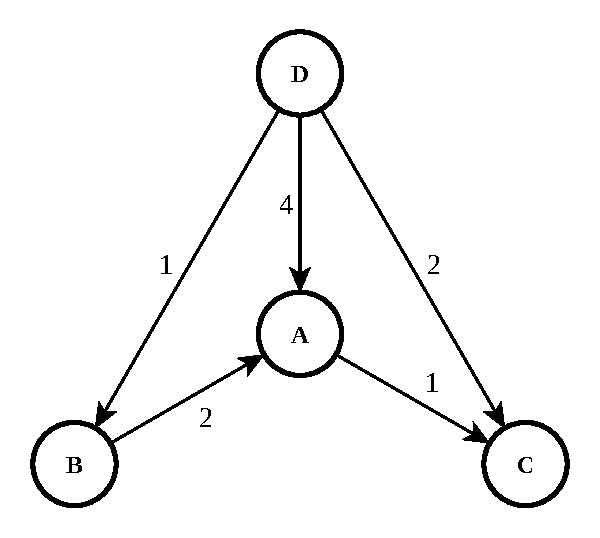
\includegraphics[width=0.5\linewidth]{graphics/graph-eg-1.pdf}
    \caption{Primjer nekonzistentnog grafa prije izračunavanja potencijala čvorova.
      U čvorove su upisane oznake vrijednosnica, a na bridove su upisane težine koje opisuju tok preferencije.}
    \label{fig:graph-eg-1}
  \end{figure}
  
  Taj graf nije konzistentan s relacijom preferencije koju predstavlja: prema njemu $B$ nije izravno usporediva s $C$, ali kako je $B \succ A$ i $A \succ C$, po tranzitivnosti bi trebalo biti i $B \succ C$, dok je prema grafu $B \sim C$.
  Također, postoje dva puta od $D$ prema $A$: to su $D \rightarrow A$ i $D \rightarrow B \rightarrow A$; duž prvog puta je zbroj težina jednak 4, a duž drugog jednak je 3, pa graf nije intrinzično konzistentan.
  Isto je i s putevima od $D$ do $C$: duž puta $D \rightarrow C$ zbroj težina jednak je 2, a duž puta $D \rightarrow B \rightarrow C$ zbroj težina jednak je 5, što je čak i veće nepodudaranje nego u prethodnom slučaju.
  
  Matrica incidencije $\matr{B}$ i vektor toka preferencije $\matr{f}$ grafa sa slike \ref{fig:graph-eg-1} su sljedeći:
  \begin{equation*}
  \matr{B} = \begin{bmatrix*}[r]
  -1 & 1 & 0 & 0 \\
  -1 & 0 & 1 & 0 \\
  -1 & 0 & 0 & 1 \\
  0 & -1 & 1 & 0 \\
  0 & -1 & 0 & 1 \\
  0 & 0 & -1 & 1
  \end{bmatrix*},\quad
  \matr{f} = \begin{bmatrix*}[r]
  -2 \\ 1 \\ -4 \\ 0 \\ -1 \\ -2
  \end{bmatrix*}
  \end{equation*}
  Matrica incidencije $\matr{B}$ konstruirana je tako da redci odgovaraju leksikografskom poretku bridova: $\overrightarrow{AB}$, $\overrightarrow{AC}$, $\overrightarrow{AD}$, $\overrightarrow{BC}$, $\overrightarrow{BD}$, i $\overrightarrow{CD}$; a stupci prirodnom poretku čvorova: $A$, $B$, $C$ i $D$.
  Istim redoslijedom i težine bridova su upisane u vektor $\matr{f}$.
  Neke težine su negativne jer se nametnuti smjer brida u matrici incidencije ne podudara sa stvarnim smjerom brida u grafu.
  
  Računanjem prema metodi potencijala $\matr{\phi^*} = \frac{1}{N}\matr{B}^\T \matr{f}$ i $\matr{f^*} = \matr{B} \matr{\phi^*}$, dobivaju se:
  \begin{equation*}
  \matr{\phi}^* = \begin{bmatrix*}[r]
  -1.25 \\ 0.75 \\ -0.25 \\ 1.75
  \end{bmatrix*}, \quad
  \matr{f}^* = \begin{bmatrix*}[r]
  -1.5 \\ -0.5 \\ -1 \\ 1 \\ -1.5 \\ -2.5
  \end{bmatrix*}
  \end{equation*}
  Prema dobivenim potencijalima čvorova $\matr{\phi}^*$ može se zaključiti kako je najviše preferiran čvor $D$, zatim $B$, zatim $C$, i naposljetku $A$.
  Rekonstrukcija grafa prikazana je na slici \ref{fig:graph-eg-2}.
  Težine u rekonstruiranom vektoru toka preferencija $\matr{f}^*$ su promijenjene u odnosu na originalni $\matr{f}$, i to je promjena veća gdje je brid uzrokovao veću nekonzistenciju u originalnom grafu --- tako je najveća promjena u težini brida $\overrightarrow{AD}$, s $-4$ na $-1$.
  Također, pojavio se i novi brid $\overrightarrow{BC}$ koji prije nije postojao u originalnom grafu.
  Smjer brida $\overrightarrow{AC}$ je preokrenut.
  Sada postoje tri puta od čvora $D$ do $A$, i duž sva tri puta zbroj težina bridova iznosi 3.
  Iz toga se vidi da je rekonstruirani graf doista intrinzično konzistentan.
  
  Mjera konzistentnosti grafa na slici \ref{fig:graph-eg-1} računa se po formuli (\ref{eq:consistency}):
  \begin{equation*}
    \kappa = \frac{\q \lVert \matr{f^*} \w \rVert}{\q \lVert \matr{f} \w \rVert} = \frac{\sqrt{13}}{\sqrt{26}} \approx 0.70711.
  \end{equation*}
  Dobivena mjera konzistentnosti manja je od 1 što potvrđuje da početni graf nije bio intrinzično konzistentan.
  Što je mjera konzistentnosti niža, to je odluka koju početni graf implicira manje pouzdana.
  
  \begin{figure}[h]
    \centering
    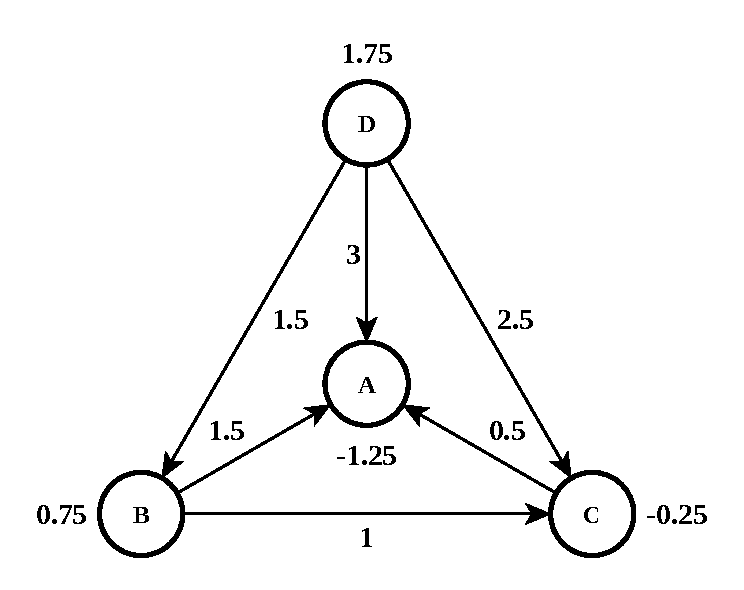
\includegraphics[width=0.619\linewidth]{graphics/graph-eg-2.pdf}
    \caption{Primjer najbliže konzistentne rekonstrukcije grafa nakon izračunavanja potencijala čvorova.}
    \label{fig:graph-eg-2}
  \end{figure}
  
  \section{Koeficijent obrtaja}
  \label{sc:turnover}
  Koeficijent obrtaja \engl{turnover ratio} je mjera koja određuje koliki udio vrijednosnica u portfelju je promijenjen između dva vremenska koraka.
  Ova mjera može biti u rasponu od 0 do 2, gdje 0 označava da su vrijednosnice u portfelju ostale iste između dva vremenska koraka, dok 2 označava da među vrijednosnicama uključenima u portfelj u prethodnom i sadašnjem koraku nijedna nije ostala ista.
  Ova mjera je važna između ostalog jer opisuje troškove trgovanja: u svakom vremenskom koraku troškovi trgovanja su direktno proporcionalni količini vrijednosnica koje su prodane ili kupljene u tom koraku.
  
  Koeficijent obrtaja $\eta^{(t)}$ u vremenskom koraku $t$ u odnosu na $t-1$ računa se na sljedeći način.
  Neka je na raspolaganju $N$ vrijednosnica.
  Vektor $\matr{\alpha}^{(t)} = \begin{bmatrix*}[r] \alpha_1^{(t)} & \alpha_2^{(t)} & \cdots & \alpha_N^{(t)} \end{bmatrix*}$ opisuje portfelj u koraku $t$; $\alpha_i^{(t)}$ predstavlja udio $i$-te vrijednosnice, te vrijedi $\alpha_i \ge 0,\ \sum_{i=1}^{N} \alpha_i = 1$.
  Tada se koeficijent obrtaja $\eta^{(t)}$ računa na način:
  \begin{equation}
  \label{eq:turnover}
  \eta^{(t)} = \sum_{i=1}^{N} \q \lvert \alpha_i^{(t)} - \alpha_i^{(t-1)} \w \rvert.
  \end{equation}
  Iz (\ref{eq:turnover}) može se vidjeti da se minimum $\eta^{(t)} = 0$ doista postiže ako i samo ako je ispunjeno $\matr{\alpha}^{(t)} = \matr{\alpha}^{(t-1)}$,
  a maksimum $\eta^{(t)} = 2$ ako i samo ako je ispunjeno $\alpha_i^{(t)} \ne 0 \Rightarrow \alpha_i^{(t - 1)} = 0$, odnosno $\alpha_i^{(t - 1)} \ne 0 \Rightarrow \alpha_i^{(t)} = 0$, jer tada vrijedi: 
  \begin{equation*}
  \eta^{(t)} = \sum_{i=1}^{N} \q \lvert \alpha_i^{(t)} - \alpha_i^{(t-1)} \w \rvert = \sum_{i=1}^{N} \q \lvert \alpha_i^{(t)}\w \rvert + \sum_{i=1}^N \q \lvert\alpha_i^{(t-1)} \w \rvert = 1 + 1 = 2.
  \end{equation*}
  
  Neka troškovi trgovanja, bilo kupovanja bilo prodavanja vrijednosnice, iznose $p$ dijelova vrijednosti po kojoj se vrijednosnica kupuje, odnosno prodaje.
  Ako se računa s logaritmima cijena umjesto s običnim cijenama, troškovi trgovanja mogu se obračunati tako da se u svakom trenutku od ostvarenog profita oduzme $p \cdot \eta^{(t)}$.
  
%  \section{Osnovni pojmovi (prebaciti na početak)}
%  
%  \begin{description}
%    \item[Vrijednosni papiri] description
%    \item[Vrijednost] description
%    \item[Cijena] description
%    \item[Povrat] description
%  \end{description} 
  
\chapter{Praktično ostvarenje algoritma trgovanja}
\label{ch:algoritam}
%  Let there be total of $N$ assets in $D$ days.
%  Let price of asset $i$ at the time step $t$ be $a_i^{\q(t\w)}$, for $i \in {\q[1, 2, \ldots, N\w]}$ and $t \in {\q[0, 1, \ldots, D-1\w]}$.
%  The log prices $b_i^{\q(t\w)}$, and log price differences $c_{i,j}^{\q(t\w)}$ between assets $i$ and $j$ are obtained as follows:
%  \begin{equation} b_i^{\q(t\w)} = \log\q(a_i^{\q(t\w)}\w) \end{equation}
%  \begin{equation} c_{i,j}^{\q(t\w)} = b_i^{\q(t\w)} - b_j^{\q(t\w)}, \end{equation}
%  and rolling means $m_{i,j}^{\q(t\w)}$ and standard deviations $d_{i,j}^{\q(t\w)}$ of log price differences over the past time window of size $T$ are obtained as follows:
  Neka u zadanom skupu podataka ima ukupno $N$ vrijednosnica označenih brojevima od $1$ do $N$, kroz $D$ vremenskih koraka.
  Ulazni podaci za algoritam čine vremenski nizovi povijesnih cijena vrijednosnica koje su na raspolaganju.
  Pretpostavka je da su vrijednosnice na tržištu likvidne, odnosno da se njima može trgovati u svakom vremenskom koraku u proizvoljnim količinama.
  Neka je s $a_i^{\q(t\w)}$ označena cijena vrijednosnice $i$ u vremenskom koraku $t$, za $i \in {\q[1, 2, \ldots, N\w]}$, i $t \in {\q[0, 1, \ldots, D-1\w]}$.
  
  Logaritamska cijena $b_i^{\q(t\w)}$ vrijednosnice $i$, i razlika logaritamskih cijena $c_{i,j}^{\q(t\w)}$ para vrijednosnica $i$ i $j$ dobivaju se na sljedeći način, $\forall i, j \in \q[1, 2, \ldots, N\w]$:
  \begin{equation}
    \label{eq:log_price}
  b_i^{\q(t\w)} = \log\q(a_i^{\q(t\w)}\w)
  \end{equation}
  \begin{equation}
    \label{eq:log_price_diff}
    c_{i,j}^{\q(t\w)} = b_i^{\q(t\w)} - b_j^{\q(t\w)}.
  \end{equation}
  Očekivanje $m_{i,j}^{\q(t\w)}$, i standardna devijacija $d_{i,j}^{\q(t\w)}$ razlika logaritamskih cijena $c_{i,j}^{\q(t\w)}$ tijekom proteklog perioda duljine $T$ procjenjuju se sljedećim izrazima:
  \begin{equation}
  \label{eq:mean}
    m_{i,j}^{\q(t\w)} = \frac{1}{T}\sum_{\tau = t - T}^{t - 1} c_{i,j}^{(\tau)}
  \end{equation}
  \begin{equation}
  \label{eq:deviation}
    d_{i,j}^{\q(t\w)} = \sqrt{\frac{1}{T - 1}\sum_{\tau=t - T}^{t - 1} \q(c_{i,j}^{(\tau)} - m_{i,j}^{\q(t\w)} \w)^2}.
  \end{equation}
  
  Procjena srednje vrijednosti u (\ref{eq:mean}) je nepristrana, što znači da je očekivanje od $m_{i,j}^{\q(t\w)}$ doista jednako srednjoj vrijednosti toga uzorka.
  Procjena standardne devijacije u (\ref{eq:deviation}) nije nepristrana, jer je dobivena korjenovanjem nepristrane procjene varijance.
  Kako je korjenovanje nelinearna operacija, ono unosi pristranost u procjenu te je ona nešto manja od veličine koju procjenjuje.
  Međutim, pristranost je manja što je broj uzoraka veći i postaje zanemariva za $T \ge 10$.
  Valja primijetiti kako je u izrazima sumiranja u (\ref{eq:mean}) i (\ref{eq:deviation}) vremenski korak $t$ namjerno izostavljen jer se radi nad proteklim periodom trajanja $T$, zbog čega sumiranje ide do $t - 1$.
%  Note that in summation used in (\ref{eq:mean}, \ref{eq:deviation}) time step $t$ was intentionally excluded, therefore summation goes only to $t - 1$.
  Izračuni (\ref{eq:log_price}) -- (\ref{eq:deviation}) su temeljni za daljnji tijek algoritma.
%  We use these calculations as basis for creating the portfolio.

%  Also note that calculating them separately for each time step $t$ is rather computationally inefficient when dealing with rolling windows of data.
%  Therefore, it is advisable to use a rolling algorithm as described in the appendix.
%  On that note, $c_{i,j}^{\q(t\w)}$, $m_{i,j}^{\q(t\w)}$, and $d_{i,j}^{\q(t\w)}$ may be more efficiently stored if stored contiguously in memory as a matrix, using following coding scheme: a pair $(i, j)$, where $i < j$, should be encoded to $k$ as:
  Također valja primijetiti da bi izračunavanje očekivanja i standardnih devijacija zasebno za svaki vremenski korak bilo računski jako neefikasno, pogotovo kada se radi o velikom skupu podataka.
  Stoga je preporučljivo koristiti algoritam za računanje s pomičnim prozorima, koji je opisan u dodatku \ref{appendix}.
  Što se tiče redukcije memorijske potrošnje, $c_{i,j}^{\q(t\w)}$, $m_{i,j}^{\q(t\w)}$, i $d_{i,j}^{\q(t\w)}$ su idejno trodimenzionalni tenzori, dimenzija $\q[(D - T) \times N \times N\w]$.
  Međutim, sva tri tenzora su simetrična ili antisimetrična, odnosno vrijedi $c_{i,j}^{\q(t\w)} = -c_{j,i}^{\q(t\w)}$, $m_{i,j}^{\q(t\w)} = -m_{j,i}^{\q(t\w)}$, i $d_{i,j}^{\q(t\w)} = d_{j,i}^{\q(t\w)}$. Stoga je polovina informacije sadržane u njima redundantna.
  Imajući to u vidu, ti tenzori se mogu gusto upakirati u matrice dimenzija $\q[(D - T) \times \q. N\cdot(N - 1) \middle/ 2\w.\w]$, koristeći sljedeće preslikavanje --- za kodiranje para $(i,j)$ u kod $k$ koristi se izraz:
  \begin{equation} k = N \cdot (i - 1) + j - 1 - \q. i \cdot (i + 1) \middle/ 2\w., \end{equation}
  a za dekodiranje $(i, j)$ iz $k$ izrazi:
  \begin{equation} i = \q \lfloor N + 1/2 - \sqrt{(N + 1/2)^2 - 2(N + k)} \w \rfloor, \end{equation}
  \begin{equation} j = k + i \cdot \q.(i + 1) \middle/ 2\w. - N \cdot (i - 1) + 1. \end{equation}
%  An example of proposed coding for $N = 5$ is shown on figure \ref{fig:coding}.
  Na slici \ref{fig:coding} prikazano je kodiranje u slučaju $N = 5$ vrijednosnica.
  
  \begin{figure}[h]
    \begin{minipage}{0.5\linewidth}
      \centering
      \begin{tabular}{C|CCCCC}
        i/j & 1 & 2 & 3 & 4 & 5 \\ \hline
        1 & \cdot & 0 & 1 & 2 & 3 \\
        2 & \cdot & \cdot & 4 & 5 & 6 \\
        3 & \cdot & \cdot & \cdot & 7 & 8 \\
        4 & \cdot & \cdot & \cdot & \cdot & 9 \\
        5 & \cdot & \cdot & \cdot & \cdot & \cdot
      \end{tabular}
    \end{minipage}%
    \begin{minipage}{0.5\linewidth}
      \centering
      \begin{tabular}{C|CCCCCCCCCC}
       k & 0 & 1 & 2 & 3 & 4 & 5 & 6 & 7 & 8 & 9 \\ \hline
       i & 1 & 1 & 1 & 1 & 2 & 2 & 2 & 3 & 3 & 4 \\
       j & 2 & 3 & 4 & 5 & 3 & 4 & 5 & 4 & 5 & 5 \\
      \end{tabular}
    \end{minipage}
    \caption{
       Primjer predložene sheme kodiranja i dekodiranja za $N = 5$.
       Točka $(\cdot)$ označava da se određena kombinacija ne koristi.
    }
    \label{fig:coding}
  \end{figure}

  \section{Konstrukcija grafa toka preferencija}
  \label{sub:creating-graph}
%  Using the obtained $c_{i,j}^{\q(t\w)}$, $m_{i,j}^{\q(t\w)}$, and $d_{i,j}^{\q(t\w)}$ it is now possible to create a graph of preference flow among assets for each time step $t$.
%  Considering one time step $t$, we find all such pairs of assets $(i,j)$ that satisfy:
%  \begin{equation}
%  \label{eq:thresh}
%  \left| c_{i,j}^{\q(t\w)} - m_{i,j}^{\q(t\w)} \right| > \alpha \cdot d_{i,j}^{\q(t\w)},
%  \end{equation}
%  i.e. current log price difference is at least $\alpha$ deviations distant from mean value of the past time window.
%  An illustration is shown on Fig. \ref{fig:devmag}.
  Korištenjem prethodno dobivenih $c_{i,j}^{\q(t\w)}$, $m_{i,j}^{\q(t\w)}$, i $d_{i,j}^{\q(t\w)}$ sada je moguće kreirati graf toka preferencija među vrijednosnicama u svakom vremenskom koraku $t$.
  Promatrajući fiksni vremenski korak $t$, izdvajaju se svi parovi vrijednosnica $(i,j)$ za koje vrijedi:
  \begin{equation}
  \label{eq:thresh}
  \q\lvert c_{i,j}^{\q(t\w)} - m_{i,j}^{\q(t\w)} \w\rvert > \beta \cdot d_{i,j}^{\q(t\w)},
  \end{equation}
  tj. trenutna apsolutna vrijednost razlike log-cijena para vrijednosnica $(i,j)$ je barem za $\beta$ standardnih devijacija udaljena od očekivanja, izmjerenih u proteklom periodu.
  Veličina $\beta$ je parametar algoritma koji se zove prag trgovanja.
  %  Parameter $\alpha$ determines how many pairs of assets should constitute the graph at current time step.
%  Afterwards, for each observed pair $(i,j)$ that exceeds the threshold we add into graph vertices $i$ and $j$, with a weighed edge of weight $w_{i,j}^{\q(t\w)}$ going from $i$ to $j$.
%  Weight $w_{i,j}^{\q(t\w)}$ is obtained as:
  Nakon toga, za svaki par $(i,j)$ koji zadovoljava (\ref{eq:thresh}) dodaju se u graf čvorovi $i$ i $j$, te brid koji ide od $i$ do $j$ s težinom $w_{i,j}^{\q(t\w)}$.
  Težina $w_{i,j}^{\q(t\w)}$ dobiva se kao:
  \begin{equation}
  \label{eq:weight}
%  w_{i,j}^{\q(t\w)} = \q. \q(c_{i,j}^{\q(t\w)} - m_{i,j}^{\q(t\w)}\w) \middle/ d_{i,j}^{\q(t\w)} \w.,
  w_{i,j}^{\q(t\w)} = \frac{c_{i,j}^{\q(t\w)} - m_{i,j}^{\q(t\w)}}{d_{i,j}^{\q(t\w)}},
  \end{equation}
  što odgovara udaljenosti razlike log-cijena od očekivanja, mjerene u standardnim devijacijama, i po apsolutnoj vrijednosti je veća od $\beta$.
  Negativan predznak težine $w_{i,j}^{\q(t\w)}$ označava da je stvarni smjer preferencije obrnut od pretpostavljenog, odnosno brid koji ide od $j$ do $i$ s pozitivnom težinom $w_{j,i}^{\q(t\w)} = -w_{i,j}^{\q(t\w)}$ ekvivalentan je prethodno pretpostavljenom bridu.
  Ilustracija ove mjere prikazana je na slici \ref{fig:devmag}.
  
  \begin{figure}[htb]
    \centering
    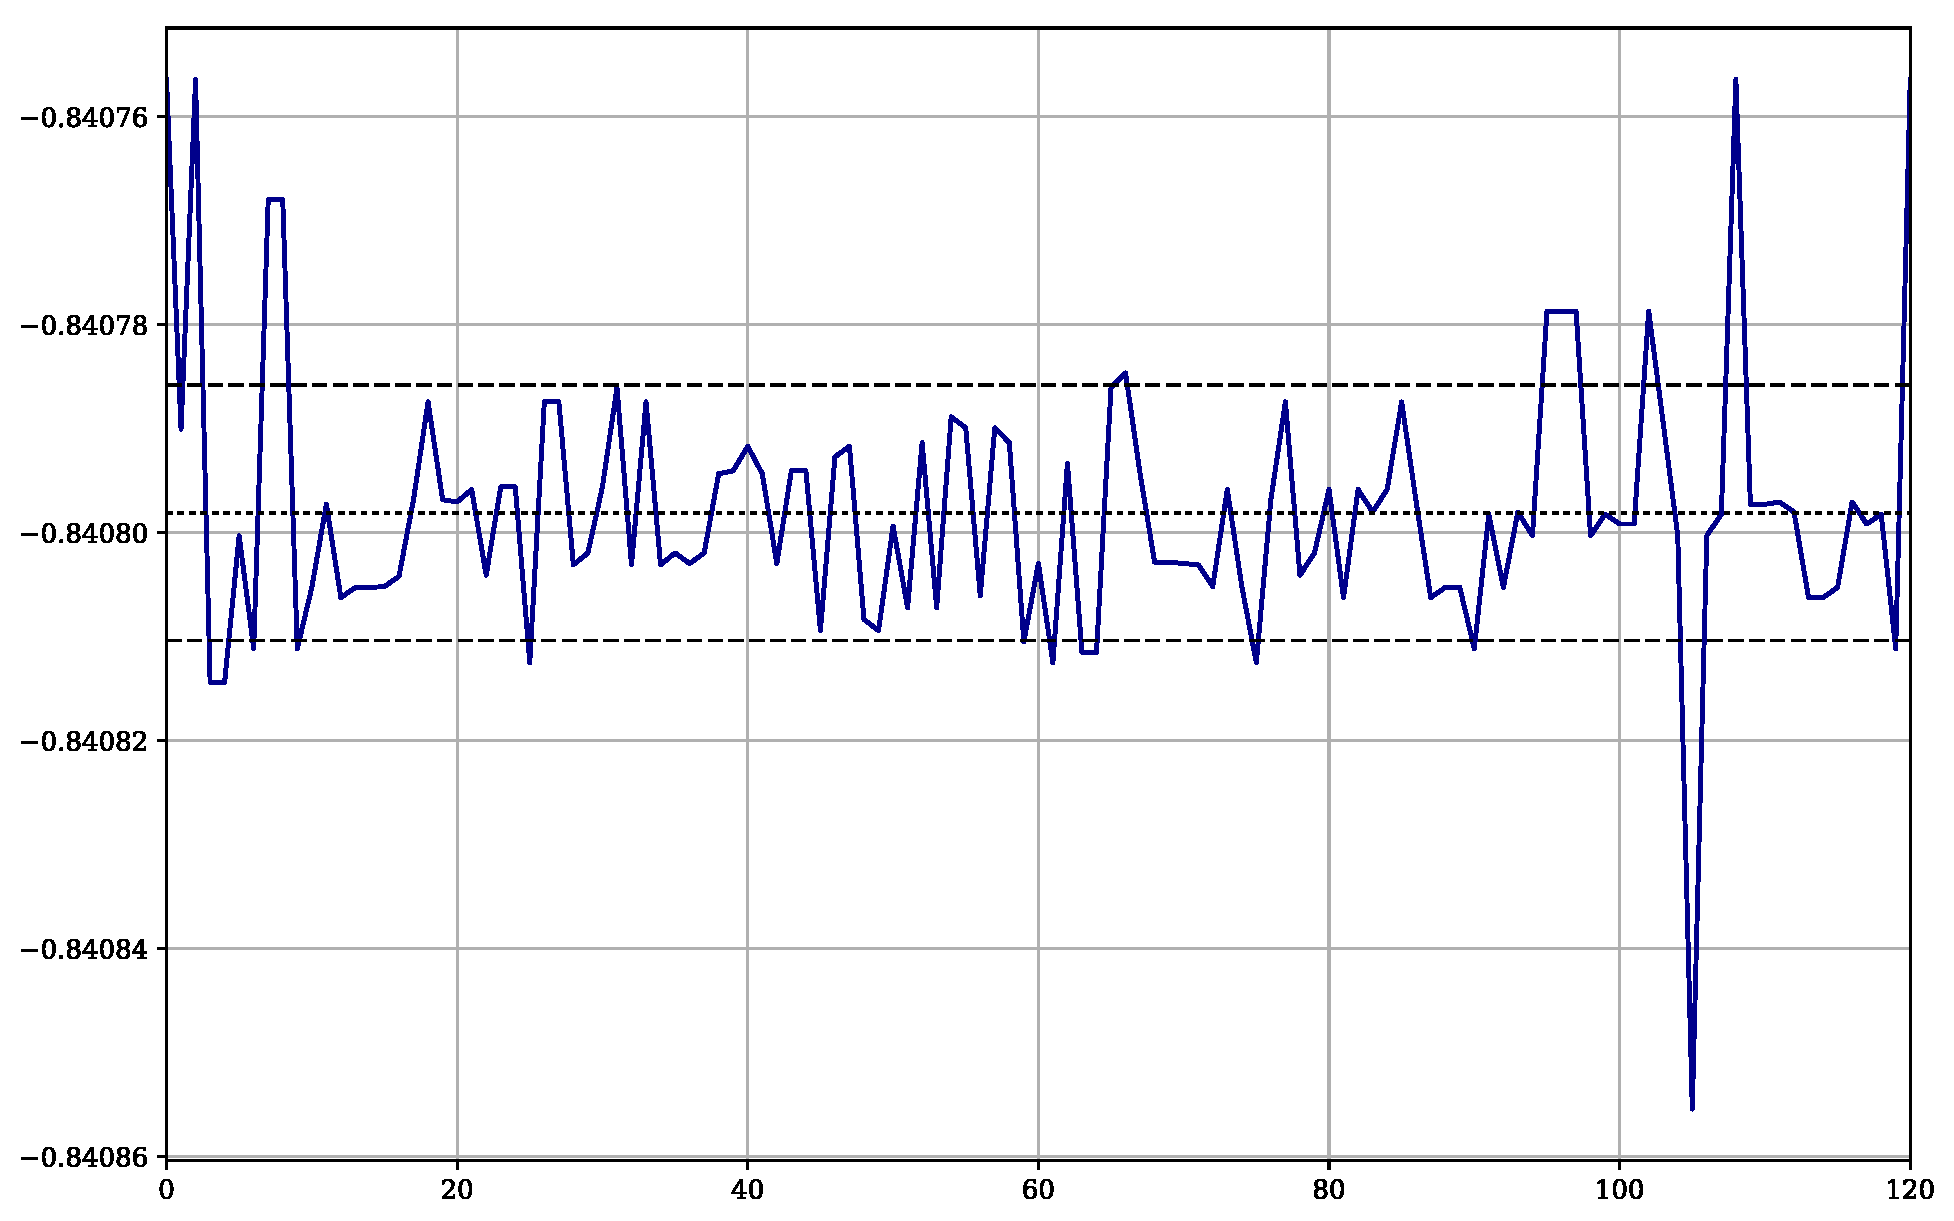
\includegraphics[width=0.9\columnwidth]{graphics/deviation-magnitude.pdf}
    \caption{
%      Log price difference between a pair of assets $(i, j)$ during a period of $T + 1$ time steps, where $T = 120$.
%      Dashed and dotted line represents mean value, and region between two dashed lines represents $\alpha$ standard deviation range from mean value, here $\alpha = 1$; both are calculated in the first $T$ time steps.
%      During the time step $T + 1$, log price difference goes over $\alpha$ standard deviations above mean value of past period of size $T$.
%      This would mean that two of the assets $i$ and $j$ would be added to the graph of preference flow at the time step $T + 1$.
%      Weight $w_{i,j}$ describes current deviation from mean value.
       Razlika log-cijena u paru vrijednosnica $(i,j)$ tijekom perioda od $T + 1$ vremenskih koraka, uz $T = 120$.
       Točka-crta linija predstavlja očekivanje, a područje između dviju crtkanih linija predstavlja $\beta$ standardnih devijacija udaljenosti od očekivanja; obje mjere su izračunate nad prvih $T$ vremenskih koraka.
       Tijekom vremenskog koraka $T + 1$, razlika log-cijena prelazi $\beta$ standardnih devijacija iznad očekivanja proteklog perioda duljine $T$.
       To znači da će vrijednosnice $i$ i $j$ biti dodane u graf toka preferencija u vremenskom koraku $T + 1$.
       Težina $w_{i,j}^{(T+1)}$ opisuje devijaciju od očekivanja.
    }
    \label{fig:devmag}
  \end{figure}
  
  Tako je moguće konstruirati graf toka preferencija za bilo koji vremenski korak $t \in \q[T, T + 1, \ldots, D-1\w]$.
  U nekim vremenskim koracima moguće je da dobiveni graf bude prazan, ako nijedan par vrijednosnica $(i,j)$ ne zadovoljava (\ref{eq:thresh}).
  Postavljanjem nižih vrijednosti za $\beta$ dobivaju se gušći grafovi i manje često se događa da je graf prazan, dok se postavljanjem $\beta = 0$ uvijek dobivaju potpuni grafovi.
%  Thus it is possible to create a graph of preference flow for each time step $t \in \q[T, T + 1, \ldots, D-1\w]$.
%  At some time steps it is possible that the graph could be empty, if it is the case that no pair $(i,j)$ satisfies (\ref{eq:thresh}).
%  Setting lower values for parameter $\alpha$ yields denser graphs, and setting $\alpha = 0$ always yields complete graphs.

  \section{Signal trgovanja}
  Signal trgovanja $\Gamma_{X, Y}^{(t)}$ između vrijednosnica $X$ i $Y$ u trenutku $t$ je funkcija koja određuje težine bridova kako je opisano u prethodnom odjeljku.
  Dobiva se na isti način kao i težine bridova:
  \begin{equation}
    \Gamma_{X, Y}^{(t)} = \frac{c_{X,Y}^{\q(t\w)} - m_{X,Y}^{\q(t\w)}}{d_{X,Y}^{\q(t\w)}},
  \end{equation}
  s bitnom razlikom da težine bridova postoje samo ako je prethodno zadovoljen prag $\beta$, a signal trgovanja je vremenski kontinuirana funkcija podložna daljnjoj analizi.
  Signal trgovanja $\Gamma_{X, Y}^{(t)}$, kao što mu i ime sugerira, opisuje željenu odluku o trgovanju vrijednosnicama $X$ i $Y$ u trenutku $t$ na način opisan tablicom \ref{table:trading-signal}.
  U područjima I i III signal je aktivan, odnosno potiče trgovanje, dok je u području II neaktivan, jer ne dopušta trgovanje.
  \begin{table}[h]
    \centering
    \caption{Opis akcija kod signala trgovanja.}
    \label{table:trading-signal}
    \begin{tabular}{cr@{}c@{}ll}
      \toprule
      područje & \multicolumn{3}{c}{uvjet} & odluka \\
      \midrule
      I & $-\infty <$ & $\,\Gamma_{X, Y}^{(t)}\,$ & $< -\beta$ & duga pozicija u $X$, kratka u $Y$ \\
      II & $-\beta \le$ & $\,\Gamma_{X, Y}^{(t)}\,$ & $\le \beta $ & nema akcije \\
      III & $\beta <$ & $\,\Gamma_{X, Y}^{(t)}\,$ & $< \infty$ & kratka pozicija u $X$, duga u $Y$ \\
      \bottomrule
    \end{tabular}
  \end{table}

  Na slici \ref{fig:trading-signal} prikazano je kretanje logaritamskih cijena vrijednosnica koje se slično ponašaju, te je vidljiv trenutak u kojem slično ponašanje prestaje, a to je trenutak kada se signal trgovanja mora aktivirati.
  Na slici \ref{fig:trading-prices} prikazan je pripadni signal trgovanja tih dviju dionica tijekom istog razdoblja s označenim aktivnim područjem.
  Naposljetku, na slici \ref{fig:trading-diffs} prikazana je razlika logaritamskih cijena tijekom istog razdoblja kako bi se lakše mogao pratiti profit ostvaren trgovanjem u skladu sa signalom trgovanja.
  \pagebreak
  \afterpage{
    
   \begin{figure}[p]
    \centering
    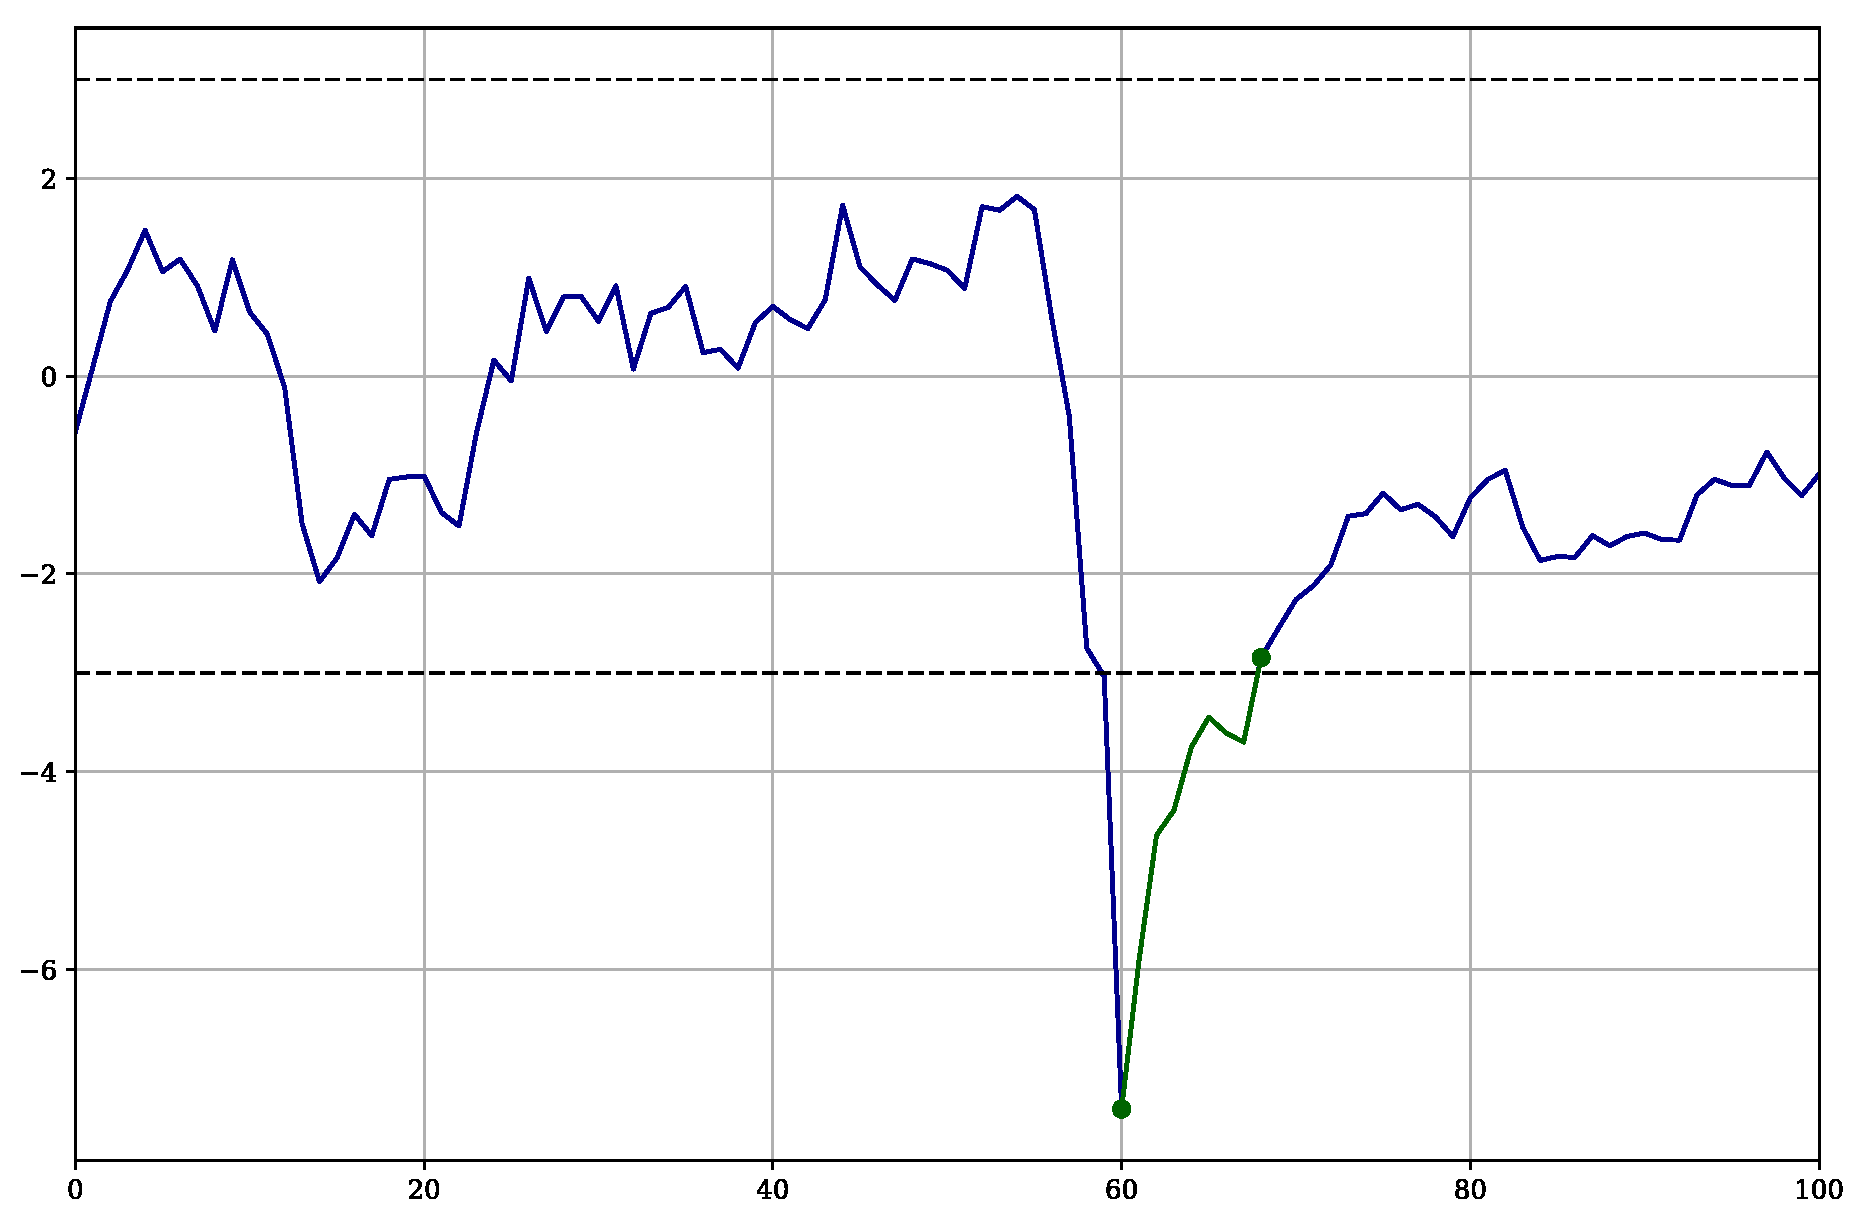
\includegraphics[width=\linewidth]{graphics/trading-prices.pdf}
    \caption{
      Signal trgovanja $\Gamma_{X, Y}^{(t)}$ za vrijednosnice $X$ i $Y$, dobiven uz korištenje $T = 120$. Prag $\beta$ je postavljen na 3. U trenutku $t_1 = 60$ (označeno prvom zelenom točkom) signal trgovanja prelazi zadani prag i ostaje u aktivnom području (čiji je razspon označen zelenom bojom) do trenutka $t_2 = 69$ (označeno drugom zelenom točkom). Kako je signal u aktivnom području manji od $-\beta$, zauzima se kratka pozicija u vrijednosnici $X$ i duga u $Y$, a po izlasku iz aktivnog područja te pozicije se zatvaraju.
      }
    \label{fig:trading-prices}
  \end{figure}
  
  \begin{figure}[p]
    \centering
    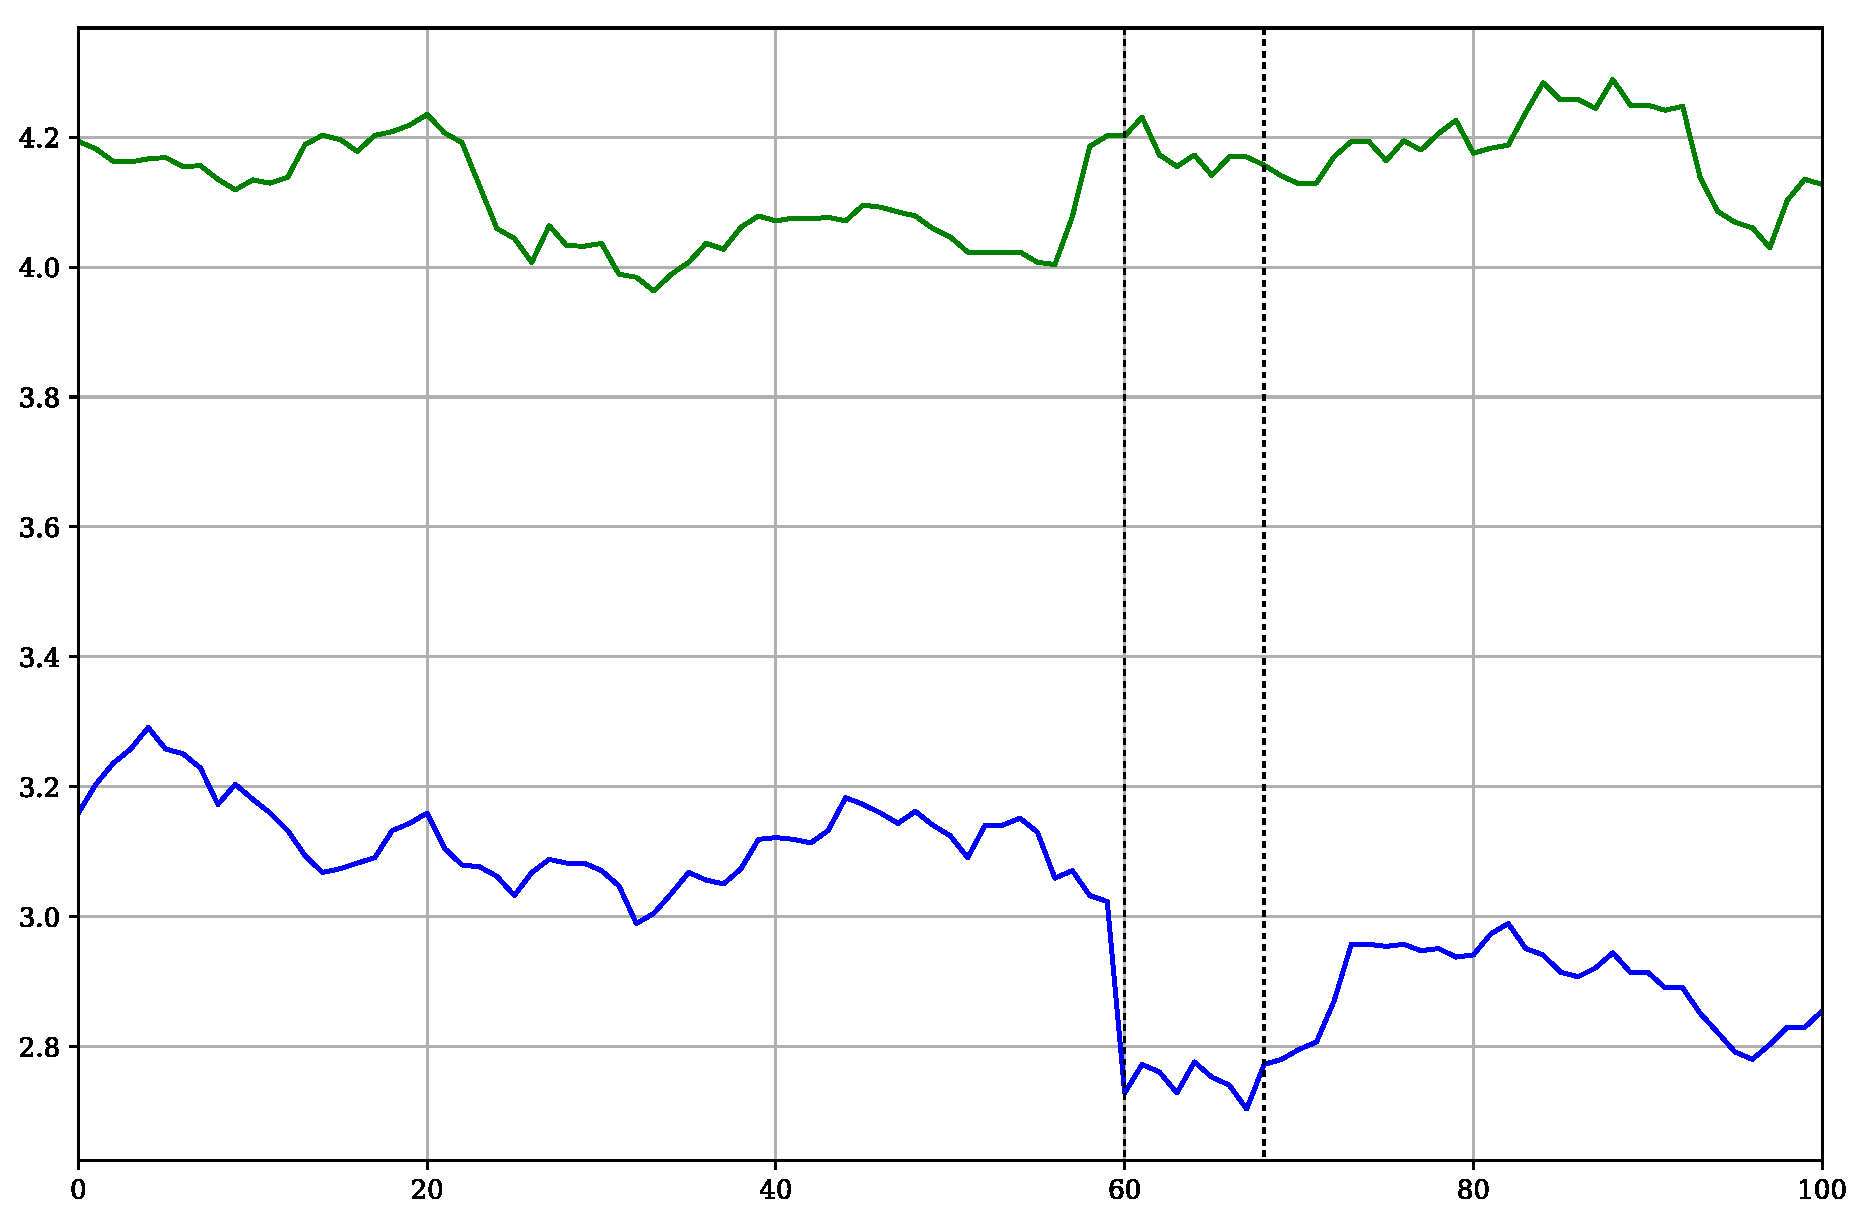
\includegraphics[width=\linewidth]{graphics/trading-signal.pdf}
    \caption{
      Kretanje logaritamskih cijena vrijednosnica $X$ (plavo) i $Y$ (zeleno).
      Između crtkanih linija nalazi se područje u kojem je signal trgovanja aktivan. Uočljiva je sličnost u kretanju cijena prije i poslije aktivnog područja signala trgovanja.}
    \label{fig:trading-signal}
  \end{figure}

  \begin{figure}[p]
    \centering
    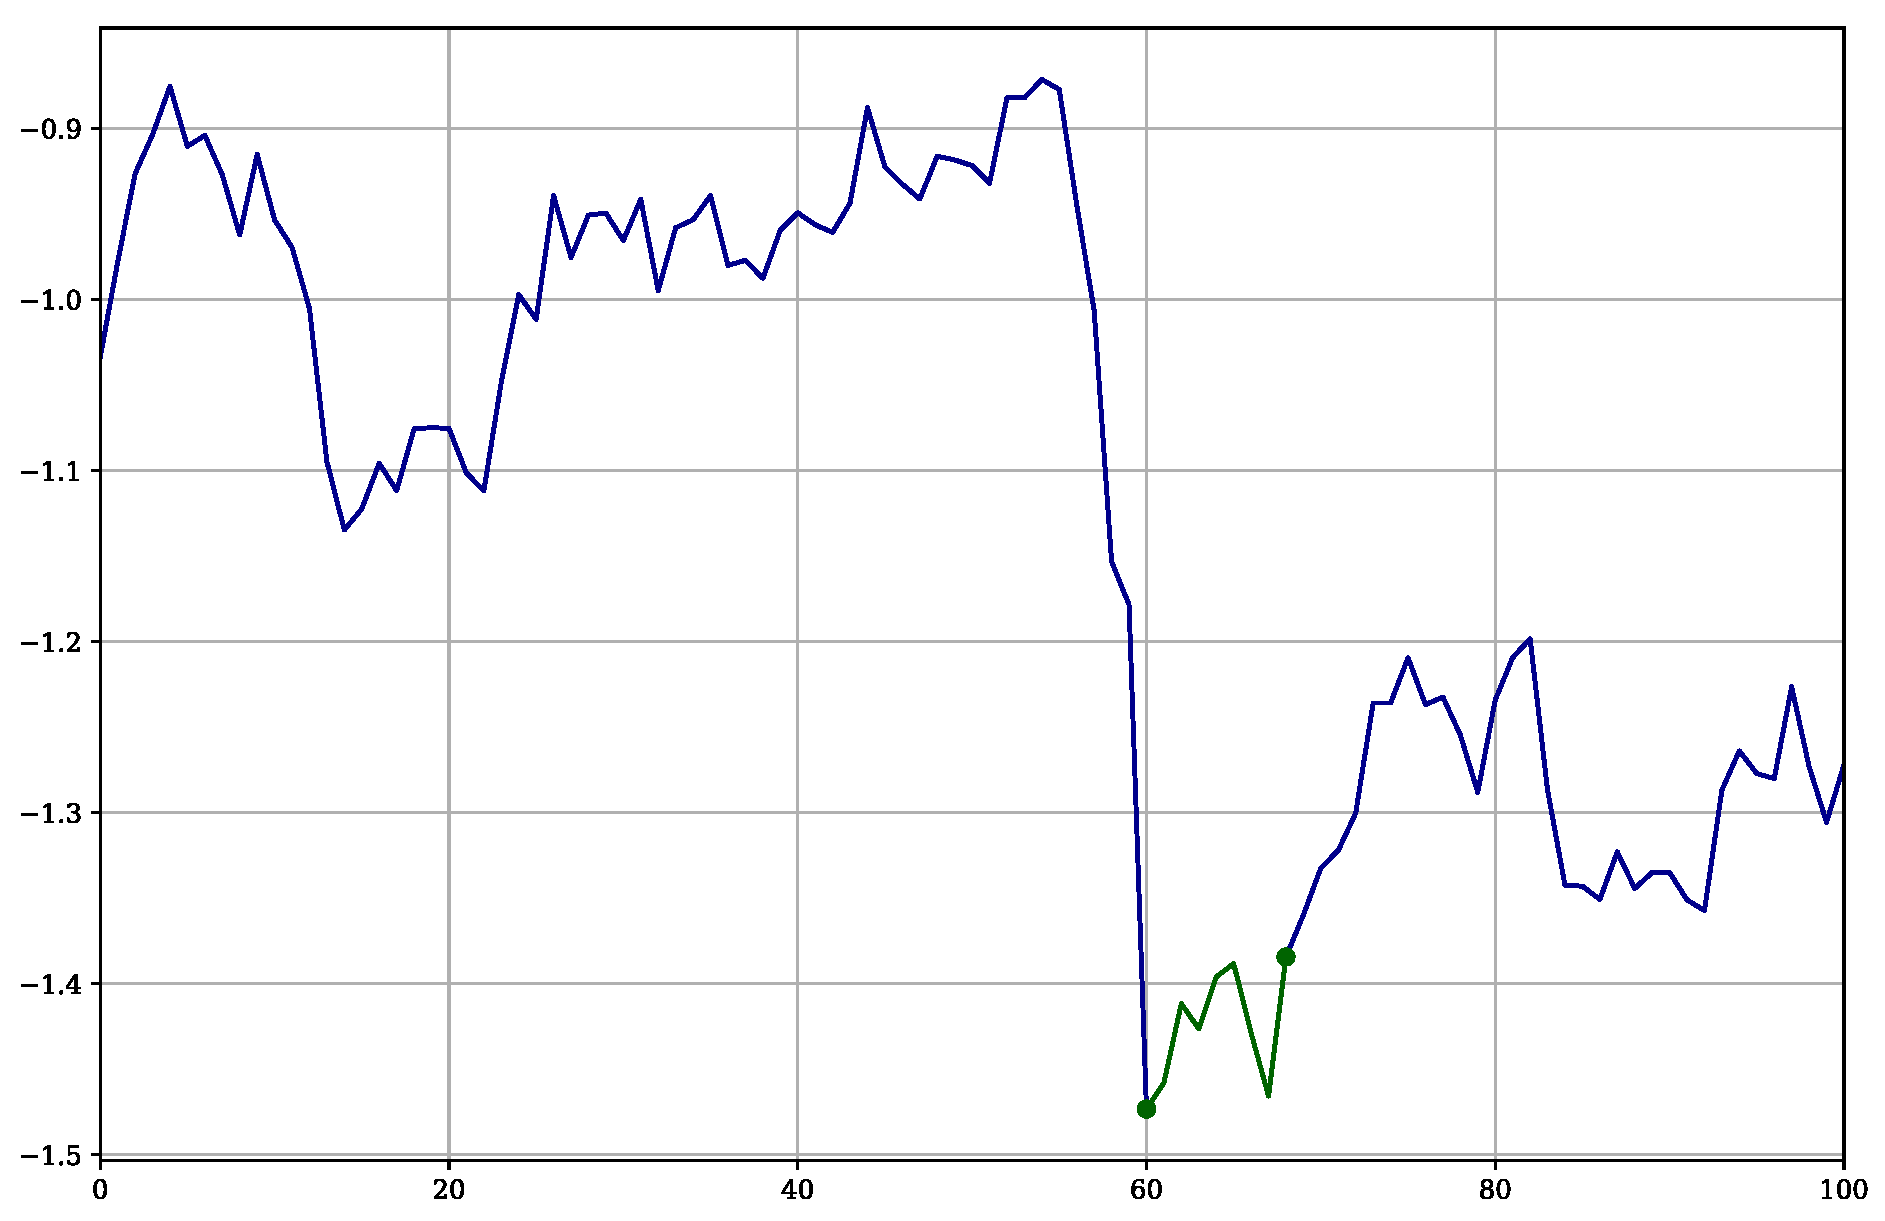
\includegraphics[width=\linewidth]{graphics/trading-diffs.pdf}
    \caption{Razlika logaritamskih cijena vrijednosnica $X$ i $Y$. Početak i kraj aktivnog područja označen je zelenim točkama. Ukupan profit jednak je razlici iznosa na kraju i iznosa na početku aktivnog područja i iznosi 0.889 u ovom primjeru.}
    \label{fig:trading-diffs}
  \end{figure}
  \clearpage
  } 

  Signal trgovanja ovisi o odabranoj veličini vremenskom prozora $T$, a odluka koju donosi dodatno ovisi o odabranom iznosu praga trgovanja $\beta$.
  Unutar iduća dva pododjeljka opisane su metode za biranje pogodnih vrijednosti za parametre $T$ i $\beta$.
  
  \subsection{Optimiranje praga trgovanja}
  U slučaju kada se trgovanje radi nad 10 ili više vrijednosnica, značajna poboljšanja mogu se postići ako se selekcija parova radi na sljedeći način.
  Za svaki par vrijednosnica $X$ i $Y$ s pripadnim cijenama $P_X^{(t)}$ i $P_Y^{(t)}$ u trenutku $t$, zahtijeva se da varijanca razlike cijena u proteklom periodu duljine $T$ bude manja od zbroja varijanci cijena pojedinačno:
  \begin{align}
  \Varfromto{\q(P_X^{(\tau)} - P_Y^{(\tau)}\w)}{t - T < \tau \le t} & <
  \Varfromto{P_X^{(\tau)}}{t - T < \tau \le t} \nonumber \\
  \label{eq:beta-cond}
  & + \Varfromto{P_Y^{(\tau)}}{t - T < \tau \le t}.
  \end{align}
  Uvjet (\ref{eq:beta-cond}) ekvivalentan je uvjetu $\Covfromto{P_X^{(\tau)},  P_Y^{(\tau)}}{t - T < \tau \le t} > 0$, jer je:
  \begin{align*}
  \Varfromto{\q(P_X^{(\tau)} - P_Y^{(\tau)}\w)}{t - T < \tau \le t} & =  \Varfromto{P_X^{(\tau)}}{t - T < \tau \le t} \\
  & + \Varfromto{P_Y^{(\tau)}}{t - T < \tau \le t} \\
  & - 2 \Covfromto{P_X^{(\tau)},  P_Y^{(\tau)}}{t - T < \tau \le t},
  \end{align*}
  ali je (\ref{eq:beta-cond}) računalno optimalniji budući da su navedene varijance već izračunate.

  \subsection{Optimiranje veličine vremenskog prozora} 
  Jedan način optimiranja veličine vremenskog prozora $T$ može se postići jednostavnom pretragom prostora vrijednosti za $T$ testiranjem nad povijesnim podacima (npr. prethodnih 1000 dana) kako bi se pronašla vrijednost $T$ koja daje najbolje kriterije (ukupan profit, ili Sharpeov omjer).
  Smislene vrijednosti parametra $T$ koje vrijedi ispitati uglavnom su veće od 30 i manje od 250 dana.
  No, kao i u prethodnom slučaju, bolji rezultati mogu se postići optimiranjem veličine prozora za svaki par vrijednosnica zasebno.
  Ispitivanje svih mogućih veličina prozora za svaki par nije izvedivo u praktičnom vremenu, stoga se mora posegnuti za nekom bržom metodom optimiranja.
  
  Testiranjem nad povijesnim podacima, prilikom trgovanja s 10 ili više vrijednosnica, empirijski je utvrđen način za poboljšanje dobivenih rezultata.
  Promatrajući signal trgovanja $\Gamma_{X, Y}$ za vrijednosnice $X$ i $Y$ određuje se vrijednost parametra $T$ koja maksimizira varijancu signala trgovanja.
  U tablici \ref{table:opt-results} prikazani su rezultati prije i poslije optimizacije praga trgovanja i veličine vremenskog prozora.
  
  \begin{table}[h]
    \centering
    \caption{Rezultati prije i poslije optimizacije parametara $T$ i $\beta$.}
    \label{table:opt-results}
    \begin{tabular}{lrr}
      \toprule
      & prije optimizacije & poslije optimizacije \\
      \midrule
      bez troškova trgovanja: & & \\
      ukupni profit & 0.32509 & 0.48489 \\
      Sharpeov omjer & 2.28115 & 3.36565 \\
      \midrule
      \multicolumn{3}{l}{uz uključene troškove trgovanja od 0.10\%:} \\
      ukupni profit & 0.17093 & 0.30617 \\
      Sharpeov omjer & 1.19602 & 2.12594 \\
      \midrule
      prosječni koeficijent obrtaja & 0.77078 & 0.89355 \\
      prosječna konzistentnost & 0.94716 & 0.67343 \\
      prosječna preciznost & 0.51500 & 0.60500 \\
      \bottomrule
    \end{tabular}
  \end{table}
  
  \section{Konstrukcija portfelja}
%  We obtain preference for each asset via the potential method, as described earlier in \ref{sub:potential}.
%  By obtaining the measure of preference for each asset it is possible to pick assets for the portfolio.
%  The most preferred assets should be bought while the least preferred should be short-sold if possible.
  Individualna mjera preferencije za svaku vrijednosnicu dobivena je metodom potencijala, na način kako je ranije opisano u \ref{sub:potential}.
  Vrijednosnice s trenutačno najvećom preferencijom preporučeno je kupiti, dok je one s najmanjom preferencijom preporučeno prodati, odnosno zauzeti kratku poziciju, ako je to moguće.
  
%  Let $\matr{\phi}^{\q(t\w)} = \begin{bmatrix} \phi_1^{\q(t\w)} & \phi_2^{\q(t\w)} & \ldots & \phi_N^{\q(t\w)} \end{bmatrix}$ denote vector of preferences of assets at time step $t$ and $\phi_i^{\q(t\w)}$ denote the preference for asset $i$ at time step $t$.
%  When picking the assets for the portfolio we take into consideration the consistency measure $\kappa$ as well.
%  Lower values of $\kappa$ suggest that we should diversify our portfolio by including some more assets in the order of preference, while higher values suggest that it is safe to do trading with smaller number of assets.
%  Portfolio diversification might be seen as a strategy for protection from fundamental risks, e.g. risk of asset default.
  Neka je $\matr{\phi}^{\q(t\w)} = \begin{bmatrix*}[r] \phi_1^{\q(t\w)} & \phi_2^{\q(t\w)} & \cdots & \phi_N^{\q(t\w)} \end{bmatrix*}$ vektor individualnih preferencija vrijednosnica u vremenskom koraku $t$, te $\phi_i^{\q(t\w)}$ predstavlja individualnu preferenciju vrijednosnice $i$ u vremenskom koraku $t$.
  Pri odabiru vrijednosnica za portfelj, u obzir se također uzima i mjera konzistentnosti $\kappa$.
  Uključivanje mjere konzistentnosti pri odabiru omogućuje zaštitu od fundamentalnog rizika (propadanja neke dionice) putem diverzifikacije portfelja.
  Interpretacija mjere konzistentnosti je sljedeća: niska mjera konzistentnosti sugerira da procjena u sadašnjem vremenskom koraku nije pouzdana, stoga je bolje diverzificirati portfelj uzimanjem većeg broja vrijednosnica, dok visoka vrijednost mjere konzistentnosti sugerira da je sigurno trgovati s manjim brojem vrijednosnica.
    
%  The bound on the assets which will be taken into portfolio is proportional to the consistency measure $\kappa$.
%  Depending on the nature of assets we may tune the consistency measure $\kappa$ to be more or less inclined to diversification by transforming it to $\kappa^\prime$:
  Granica mjere preferencije za vrijednosnice koje će biti uključene u portfelj je proporcionalna mjeri konzistentnosti $\kappa$.
  Ovisno o prirodi skupa vrijednosnica koji je na raspolaganju, mjera konzistentnosti može se preinačiti tako da algoritam bude više ili manje sklon diverzifikaciji portfelja, na sljedeći način:
  \begin{equation}
  \kappa^\prime = a + (1 - a)\cdot \kappa^b,
  \end{equation}
  gdje je $a \in [0, 1], b \in \mathbb{R}^+$.
  Za vrijednosti $a = 0$, $b = 1$, $\kappa^\prime$ postaje jednak $\kappa$.
  Parametar $a$ regulira utjecaj mjere konzistentnosti na određivanje portfelja: za $a = 0$, diverzifikacija u potpunosti ovisi o mjeri konzistentnosti $\kappa$, dok za $a = 1$ mjera konzistentnosti ne dolazi do izražaja te se u portfelju zadržava samo vrijednosnica s najvećom individualnom preferencijom.
  S druge strane, parametar $b$ regulira diverzifikaciju portfelja: kada je $0 < b < 1$, algoritam je manje privržen diverzifikaciji čak i kada je konzistentnost mala, a kada je $b > 1$, algoritam je više privržen diverzifikaciji čak i kada je mjera konzistentnosti velika.
  
%  For determining the assets that should be held in the portfolio at time step $t$, we find such assets $i$ for which holds:
  Duga pozicija zauzima se u vrijednosnicama $i$ za koje u vremenskom koraku $t$ vrijedi:
  \begin{equation*}
  \phi_i^{\q(t\w)} \ge \kappa^\prime \cdot \Phi_\mathit{max}^{(t)},
  \end{equation*}
  gdje je $\Phi_\mathit{max}^{(t)} = \max_j \q\{ \q\lvert \phi_j^{(t)} \w\rvert \w\}$, maksimum po apsolutnoj vrijednosti.
  Isto tako, kratka pozicija zauzima se u onim vrijednosnicama $i$ za koje u vremenskom koraku $t$ vrijedi:
  \begin{equation*}
  \phi_i^{\q(t\w)} \le -\kappa^\prime \cdot \Phi_\mathit{max}^{(t)}.
  \end{equation*}
  
  Ponekad je poželjno koristiti alternativnu strategiju za odabir vrijednosnica koja u svakom trenutku koristi fiksan broj vrijednosnica u portfelju.
  Neka je željeni broj vrijednosnica označen sa $q > 0$.
  Prag $\Phi_q^{(t)}$ određuje se kao $q$-ta po apsolutnoj vrijednosti najveća mjera preferencije u vektoru $\matr{\phi^{(t)}}$:
  \begin{gather*}
  \Phi_q^{(t)} = \begin{cases}
  \Phi_\mathit{max}^{(t)}, & q = 1, \\
  \absmax \q\{ \matr{\phi^{(t)}}\, \middle\backslash\, \q\{ \q. \Phi_i^{(t)} \middle| 1 \le i < q \w. \w\} \w\}, & q > 1,
  \end{cases}
  \end{gather*}
  gdje je $\absmax \q\{ \cdot \w\}$ maksimum po apsolutnoj vrijednosti.
  Duga pozicija zauzima se u vrijednosnicama $i$ za koje u vremenskom koraku $t$ vrijedi:
  \begin{equation*}
  \phi_i^{\q(t\w)} \ge \Phi_q^{(t)},
  \end{equation*}
  i kratka pozicija u vrijednosnicama $i$ za koje u vremenskom koraku $t$ vrijedi:
  \begin{equation*}
  \phi_i^{\q(t\w)} \le -\Phi_q^{(t)}.
  \end{equation*}
  
%  For $a = 0$ diversification completely depends on consistency $\kappa$, while for $a = 1$ only the most preferred asset is held in the portfolio (no diversification).
%  On the other hand, when $0 < b < 1$, algorithm is less inclined to diversification even when consistency is low, and when $b > 1$, algorithm is more inclined to diversification even when consistency is high.

  \section{Testiranje}
  Simulacija algoritma trgovanja implementirana je u programskom jeziku \textit{Python 3} uz korištenje standardnog paketa znanstvenih računalnih alata za \textit{Python}, \textit{SciPy} \citep{scipy}.
  Ključne komponente tog paketa uključuju:
  \begin{description}
    \item[\textit{NumPy}] Standardna biblioteka za računanje, koja je optimirana za efikasno računanje nad matricama i vektorima.
    \item[\textit{pandas}] Nadogradnja nad \textit{NumPy} biblioteku koja donosi naprednije podatkovne strukture, te mogućnost čitanja i pisanja u raznovrsne datotečne formate.
    \item[\textit{SciPy}] Kolekcija efikasnih algoritama iz linearne algebre, statistike, obrade signala, optimizacije i ostaloga, koji koriste \textit{NumPy}.
    \item[\textit{Matplotlib}] Biblioteka koja pruža podršku za prikazivanje podataka u obliku raznih vrsta grafova.
  \end{description}
  Uz navedene komponente korišten je i \textit{Jupyter} poslužitelj koji pruža mogućnost rada u zasebnim bilježnicama u kojima je moguće interaktivno pokretati napisani kod i pregledavati dobivene rezultate.
  Svi korišteni alati su otvorenog koda.
  U svrhu testiranja rada algoritma implementirane su dolje navedene pomoćne funkcije.

  \begin{description}
    \item[Računanje srednje vrijednosti i varijance na pomičnom prozoru]
  \end{description}
  \begin{lstlisting}[language=Python, basicstyle=\footnotesize\ttfamily]
  def rolling_mean_variance(series, T, weight=1.0,
                            return_stds=False):
    """
    Calculates mean and variance of time series on rolling windows.
    :param series: 2D matrix of multiple time series packed in
    columns.
    :param T: size of rolling window.
    :param weight: (optional) for exponential mean and average.
    :param return_stds: return standard deviation instead of 
    variance.
    :return: a tuple consisting of mean and variance.
    """
    L, N = series.shape
    if L < T:
      return np.empty((0, N)), np.empty((0, N))
      
    init_ws = np.tile(np.array([[weight ** i
                                 for i in range(T - 2, -1, -1)]]
                               ).transpose(), [1, N])
    mean = np.zeros((L - T + 1, N))
    var = np.zeros((L - T + 1, N))
    s0 = ((np.sum(init_ws[:, 0]) + weight ** (T - 1)) 
          * np.ones((1, N)))
    s1 = np.sum(series[:T - 1, :] * init_ws, axis=0,
                keepdims=True)
    s2 = np.sum(series[:T - 1, :] ** 2 * init_ws, axis=0,
                keepdims=True)
    s1_prev = np.zeros((1, N))
    s2_prev = np.zeros((1, N))
    for i in range(L - T + 1):
      s1 *= weight
      s2 *= weight
      s1 += series[i + T - 1, :] - s1_prev * weight ** T
      s2 += series[i + T - 1, :] ** 2 - s2_prev * weight ** T
      s1_prev = series[i, :]
      s2_prev = series[i, :] ** 2
      mean[i, :] = s1 / s0
      var[i, :] = (s0 * s2 - s1 * s1) / (s0 * (s0 - 1))
    return (mean, var) if not return_stds else (mean, np.sqrt(var))
  \end{lstlisting}
  \begin{description}
    \item[Računanje koeficijenata obrtaja]
  \end{description}
  \begin{lstlisting}[language=Python, basicstyle=\footnotesize\ttfamily]
  def turnover_ratio(series):
    """
    Calculates turnover ratio.
    :param series: list of sets of assets
    :return: list of turnover ratios
    """
    turnovers = []
    S1 = set()
    for S2 in (set(s) for s in series):
      lS1 = len(S1)
      lS2 = len(S2)
      turnover = 0
      if lS1:
        turnover += len(S1 - S2) / lS1
      if lS2:
        turnover += len(S2 - S1) / lS2
      if lS1 and lS2:
        turnover += len(S1 & S2) * abs(1 / lS1 - 1 / lS2)
      turnovers += [turnover]
      S1 = S2
    return np.array(turnovers)
  \end{lstlisting}
  \begin{description}
    \item[Algoritam statističke arbitraže]
  \end{description}
  \begin{lstlisting}[language=Python, basicstyle=\footnotesize\ttfamily]
  def stat_arb(log_prices, T, d='filtered',
               return_trading_signal=False, v=0.0,
               trading_signal=None):
    """
    Statistical arbitrage algorithm. 
    :param log_prices: assets log price series
    :param T: windows size
    :param d: selection threshold, real number or 'filtered' if using
    selection based on change of variance 
    :param return_trading_signal: (optional) include return trading
    signal in returned values
    :param v: (optional) portion of most volatile assets that should
    be discarded 
    :param trading_signal: supply precalculated trading signal 
    :return: triple containing list of timestamps, list of coded
    pairs and list of weights
    """
    N = log_prices.shape[1]
    log_pairs = calculate_pairwise_diffs(log_prices)
    _, std_prices = rolling_mean_variance(log_prices, T,
                                          return_stds=True)
    mean_pairs, std_pairs = rolling_mean_variance(log_pairs, T,
                                                  return_stds=True)
    if trading_signal is None:
      trading_signal = ((log_pairs[T:] - mean_pairs[:-1])
                        / std_pairs[:-1])

    cond = None
    if d == 'filtered':
      trading_threshold = np.array([np.sqrt(std_prices[:-1, i] ** 2
                                            + std_prices[:-1, j] ** 2)
                                            for i in range(N)
                                            for j in range(i + 1, N)]
                                   ).transpose()
      cond = std_pairs[:-1] <= trading_threshold
    elif isinstance(d, numbers.Number):
      cond = np.abs(trading_signal) >= d
    else:
      raise ValueError('d must be "filtered" or number.')
    if v != 0.0:
      most_volatile = np.argsort(std_prices, axis=1)[:, -int(v * N):]
      make_pairs = lambda row: [encode_pair(i + 1, j + 1, N)
                                for ii, i in enumerate(row)
                                for j in row[ii + 1:]]
      most_volatile_pairs = np.apply_along_axis(make_pairs, 1,
                                                most_volatile)
      if most_volatile_pairs.shape[1] != 0:
        cond[:, most_volatile_pairs] = False
        
    cond[std_pairs[:-1] == 0] = False
    ts, codes = np.where(cond)
    weights = trading_signal[ts, codes]
    ts += T
    return_values = (ts, codes, weights)
    if return_trading_signal:
      return_values += (trading_signal,)
    return return_values
  \end{lstlisting}
    
  \chapter{Rezultati}
  \label{ch:rezultati}
  \section{S\&P 203}
  Skup podataka nad kojim je algoritam testiran je podskup koji sadrži 203 od 500 dionica koje su bile kontinuirano uključene u S\&P 500 indeks u razdoblju od 1. siječnja 1980. do 31. prosinca 2003.
  Razdoblje uključuje 6261 dan trgovanja, odnosno vremenskih koraka.
  Ukupno 20503 parova dionica je ispitano metodom statističke arbitraže u svakom vremenskom koraku.
  Simulirani su troškovi trgovanja u iznosu 0.10\% za svako obavljeno trgovanje.
  Sažeti prikaz rezultat dan je u tablici \ref{table:results-1}.
  
  Godišnji Sharpeov omjer $S$ definiran je kao omjer srednjeg godišnjeg povrata $\mu_r$ i srednje godišnje volatilnosti $\sigma_r$.
  Analizirana su zasebno trgovanja koja rezultiraju pozitivnim i negativnim profitom, njihova razlika i omjer.
  Mjera točnosti definirana je kao omjer broja trgovanja koja rezultiraju pozitivnim profitom u ukupnom broju trgovanja.
  Mjera obrtaja \engl{turnover ratio} opisuje promjenu portfelja između dva vremenska koraka.
  Ova mjera može biti u rasponu od 0 do 2, gdje vrijednost 0 znači da nema promjene, vrijednost 1 odgovara prelasku iz ili u prazan portfelj, a vrijednost 2 znači da su vrijednosnice između dva vremenska koraka potpuno različite.
  Na kraju je izračunat i ukupan profit uz uključene troškove trgovanja.
  
%We test the proposed method on a set of 203 stocks that were contiguously included in S&P 500 index from Jan 1st, 1980 thru Dec 31st, 2003, which includes 6261 trading days.
%A total of 20503 pairs of assets were probed for statistical arbitrage at each time step.
%Transaction costs of 0.10% were also included in the analysis.
%The summary of results for various parameters is shown in Table I.
%The annual Sharpe ratio [11] is defined as: S = μ σ r r – the ratio between annual mean returns and volatilities of the considered portfolio.
%For each individual trade we analyze the profit by evaluating the amount of gain, loss and net profit, as well as gain/loss ratio.
%We measure the algorithm accuracy as the ratio of trades resulting in gain to the total number of trades, and we calculate the average turnover ratio as the average percetnage of the portfolio which needs to be rebalanced at each point.
%Finally, we include the transaction costs and recalculate the portfolio gains.
%The highest profits and Sharpe ratios have been achieved when using α = 0.
%These results indicate that the proposed method does indeed yield portfolios which are able to perform mutli–criteria statistical arbitrage on a large set of assets.
%In addition, we report that the method adapts to the inconsistence of preferences by picking variable number of assets into the portfolio.
%This speaks to the resilience of the algorithm to various market conditions, also demonstrated by the obtained portfolio performance.
%Another interesting finding is the fact that the average gain is much higher than the average loss, meaning that the algorithm errors cost less than the gains obtained when the algorithm is correct.
%The method is shown to produce rational turnover ratios, and the fact that the obtained Sharpe ratios remain high despite transaction costs additionally affirms the validity of the approach
%These findings suggest that the proposed method produces consistent returns and may be feasible in a live market setting.
  
  \begin{figure}[p]
    \centering
    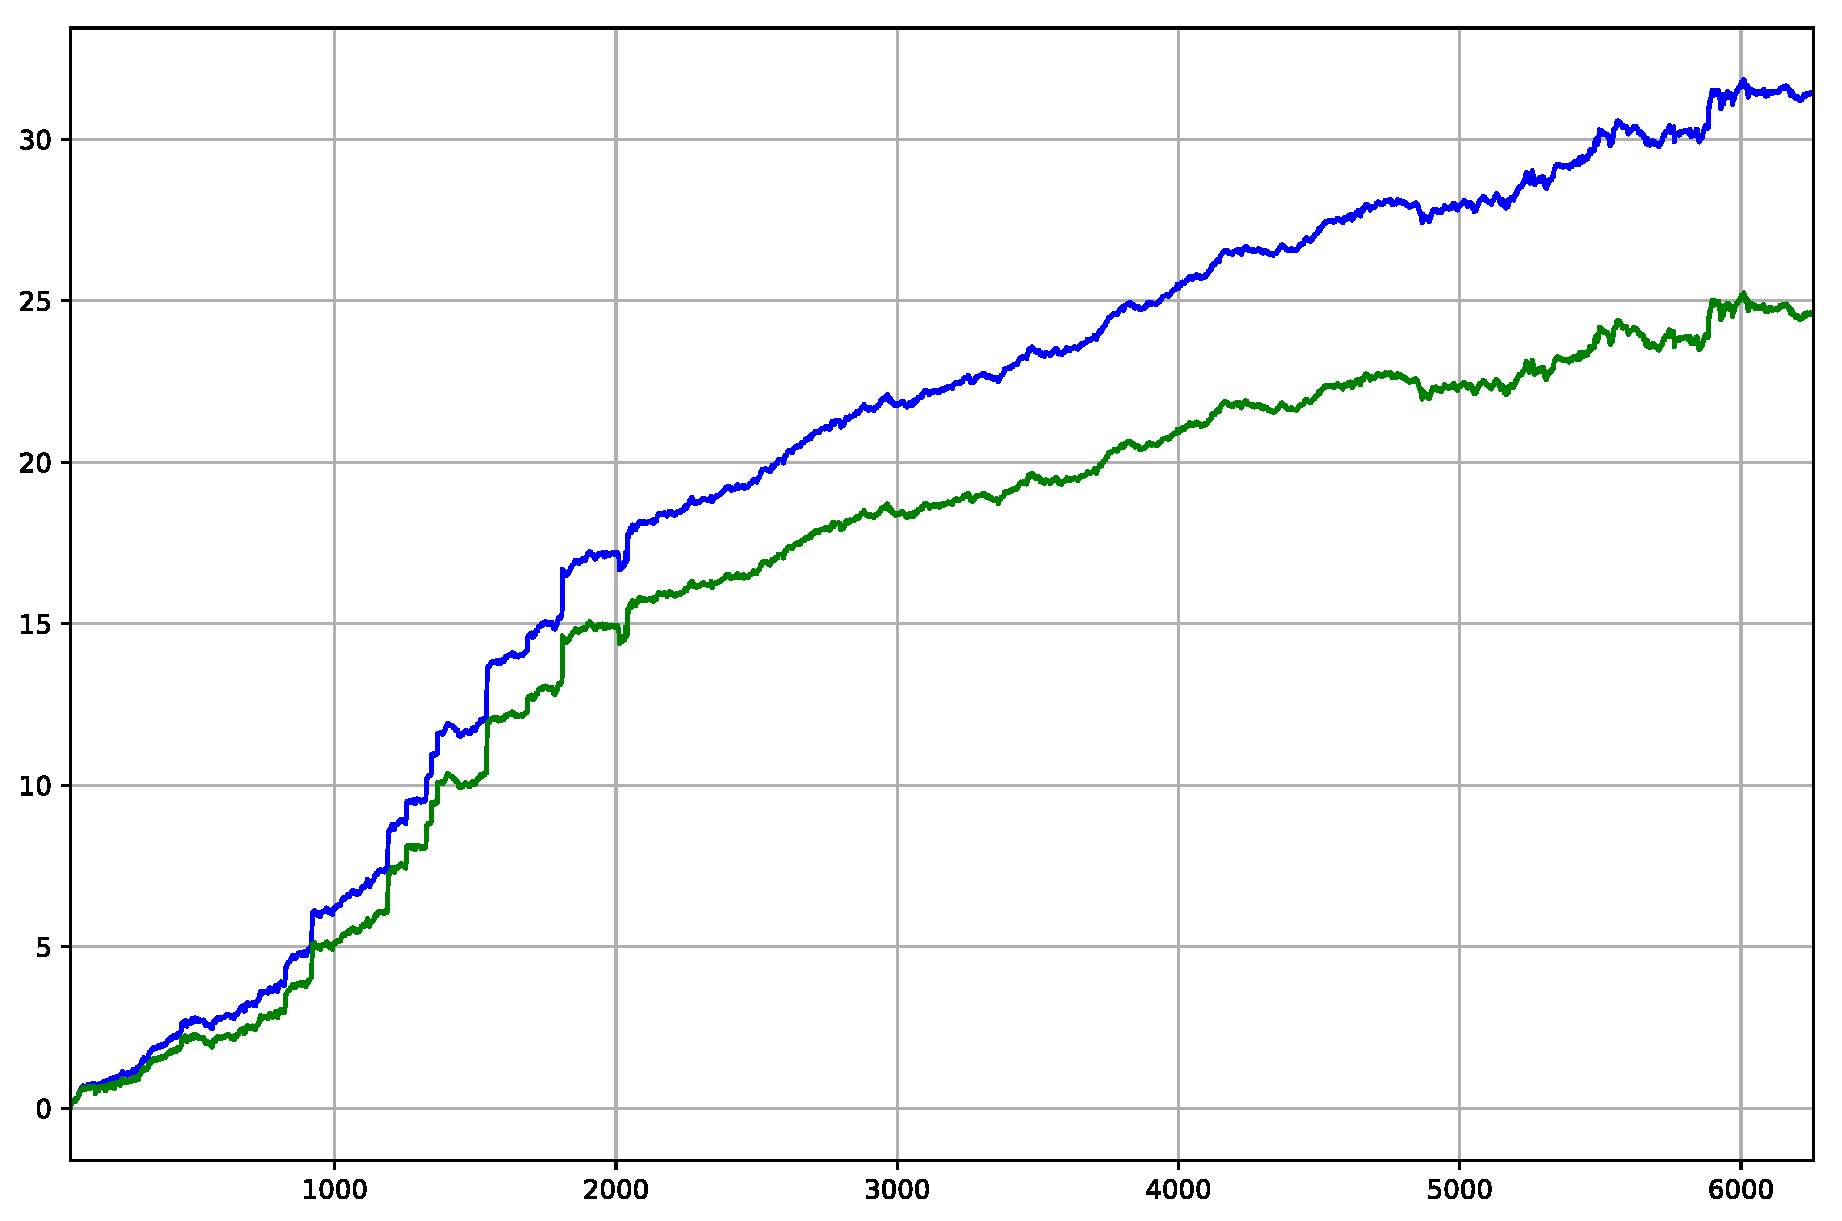
\includegraphics[width=\linewidth]{graphics/results1.pdf}
    \caption{Rezultati simulacija trgovanja nad podskupom dionica S\&P 500 indeksa. Plavom bojom je prikazana krivulja kumulativnog profita bez uključenih troškova trgovanja, a zelenom uz uključene troškove trgovanja od 0.10\% po transakciji.}
    \label{fig:result1}
  \end{figure}

  \begin{figure}[p]
    \centering
    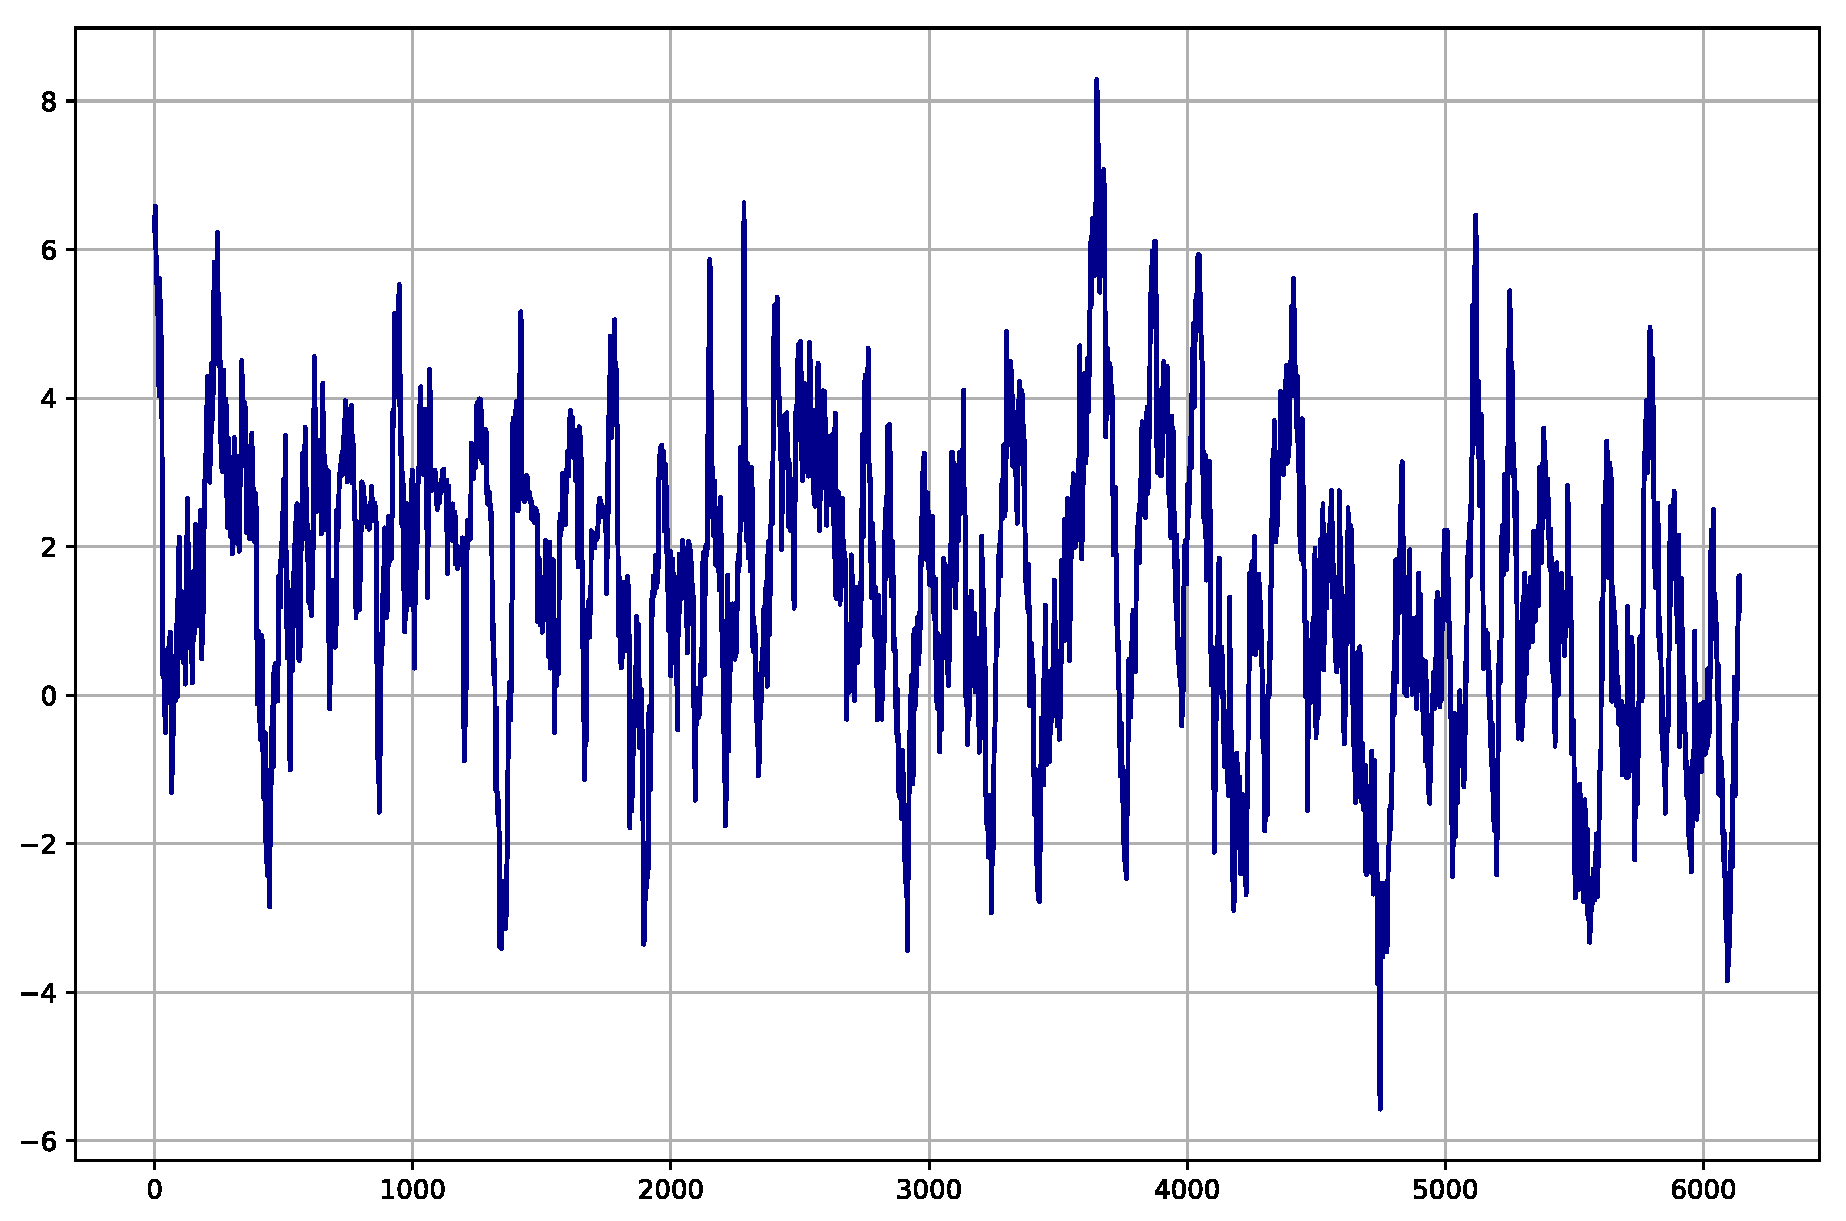
\includegraphics[width=\linewidth]{graphics/sharpe1.pdf}
    \caption{Sharpeov omjer izražen na godišnjoj razini, na prozorima veličine $T = 60$, za simulaciju trgovanja nad podskupom dionica S\&P 500 indeksa.}
    \label{fig:sharpe1}
  \end{figure}

  \begin{sidewaystable}[p]
  \centering
  \captionof{table}{Rezultati testiranja nad S\&P 203 skupu, uz $T = 60, \beta=0$.}
  \label{table:results-1}
  \begin{tabularx}{\hsize}{Xrrrrrrr}
    \toprule
    Parametar: & & & & & & & \\
    \quad a & \multicolumn{3}{c}{0.0} & \multicolumn{3}{c}{0.5} & \multicolumn{1}{c}{1.0} \\ \cmidrule(lr){2-4} \cmidrule(lr){5-7} \cmidrule(lr){8-8}
    \quad b & \multicolumn{1}{c}{0.5} & \multicolumn{1}{c}{1.0} & \multicolumn{1}{c}{2.0} & \multicolumn{1}{c}{0.5} & \multicolumn{1}{c}{1.0} & \multicolumn{1}{c}{2.0} & \multicolumn{1}{c}{/} \\ \midrule
    Prosječni povrat (godišnji) & 0.95339 & 0.88967 & 0.84463 & 0.98336 & 0.95663 & 0.89704 & 1.00223 \\
    Volatilnost (godišnja) & 0.77042 & 0.76595 & 0.74077 & 0.77905 & 0.77054 & 0.76660 & 0.78363 \\
    Sharpeov omjer (godišnji) & 1.23750 & 1.16152 & 1.14020 & 1.26225 & 1.24150 & 1.17015 & 1.27896 \\ \midrule
    Profit: &  &  &  &  &  &  &  \\
    \quad samo pozitivan & 89.27624 & 88.89440 & 88.32548 & 89.58775 & 89.29840 & 89.04414 & 89.55020 \\
    \quad samo negativan & -58.37779 & -59.03715 & -58.41396 & -58.24852 & -58.32385 & -59.02220 & -58.05316 \\
    \quad ukupan & 30.89846 & 29.85725 & 29.91152 & 31.33923 & 30.97456 & 30.02195 & 31.49704 \\
    \quad omjer pozitivnog i negativnog & 1.52928 & 1.50574 & 1.51206 & 1.53803 & 1.53108 & 1.50866 & 1.54256 \\ \midrule
    Prosječna točnost & 0.36485 & 0.39276 & 0.43413 & 0.34902 & 0.36458 & 0.39145 & 0.33241 \\
    Prosječni koeficijent obrtaja & 0.59976 & 0.64224 & 0.73597 & 0.57585 & 0.59947 & 0.64089 & 0.55112 \\ \midrule
    Stvarni profit, uz troškove trgovanja od 0.10\% & 23.46019 & 21.89215 & 20.78402 & 24.19757 & 23.53996 & 22.07361 & 24.66204 \\
    \bottomrule
  \end{tabularx}
\end{sidewaystable}

  \pagebreak
  
  \section{S\&P 500}
  \todo
  Rezultati testiranja nad punim S\&P indeksom. \\
  slike i tablica.

  \begin{figure}[p]
    \centering
    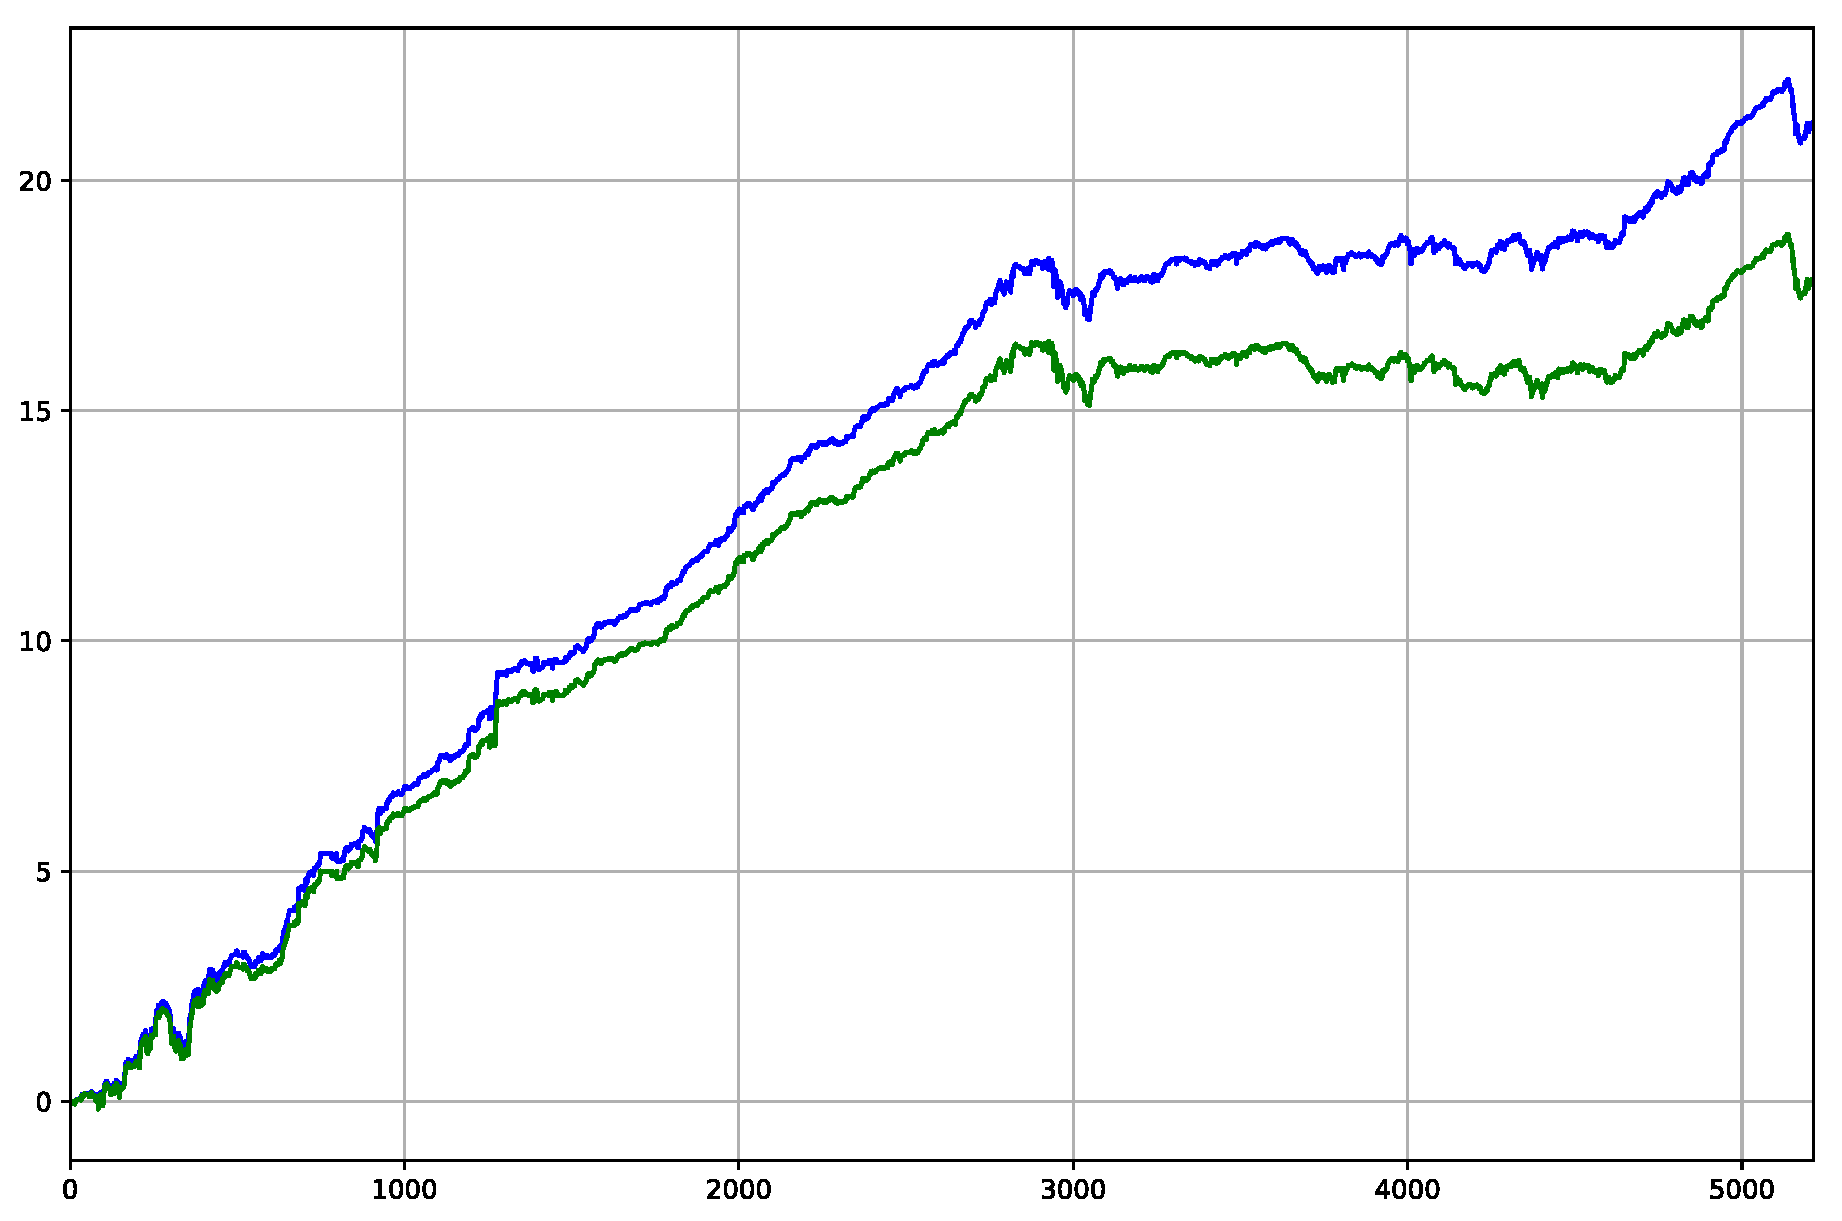
\includegraphics[width=\linewidth]{graphics/results2.pdf}
    \caption{}
    \label{fig:results2}
  \end{figure}

  \begin{figure}[p]
    \centering
    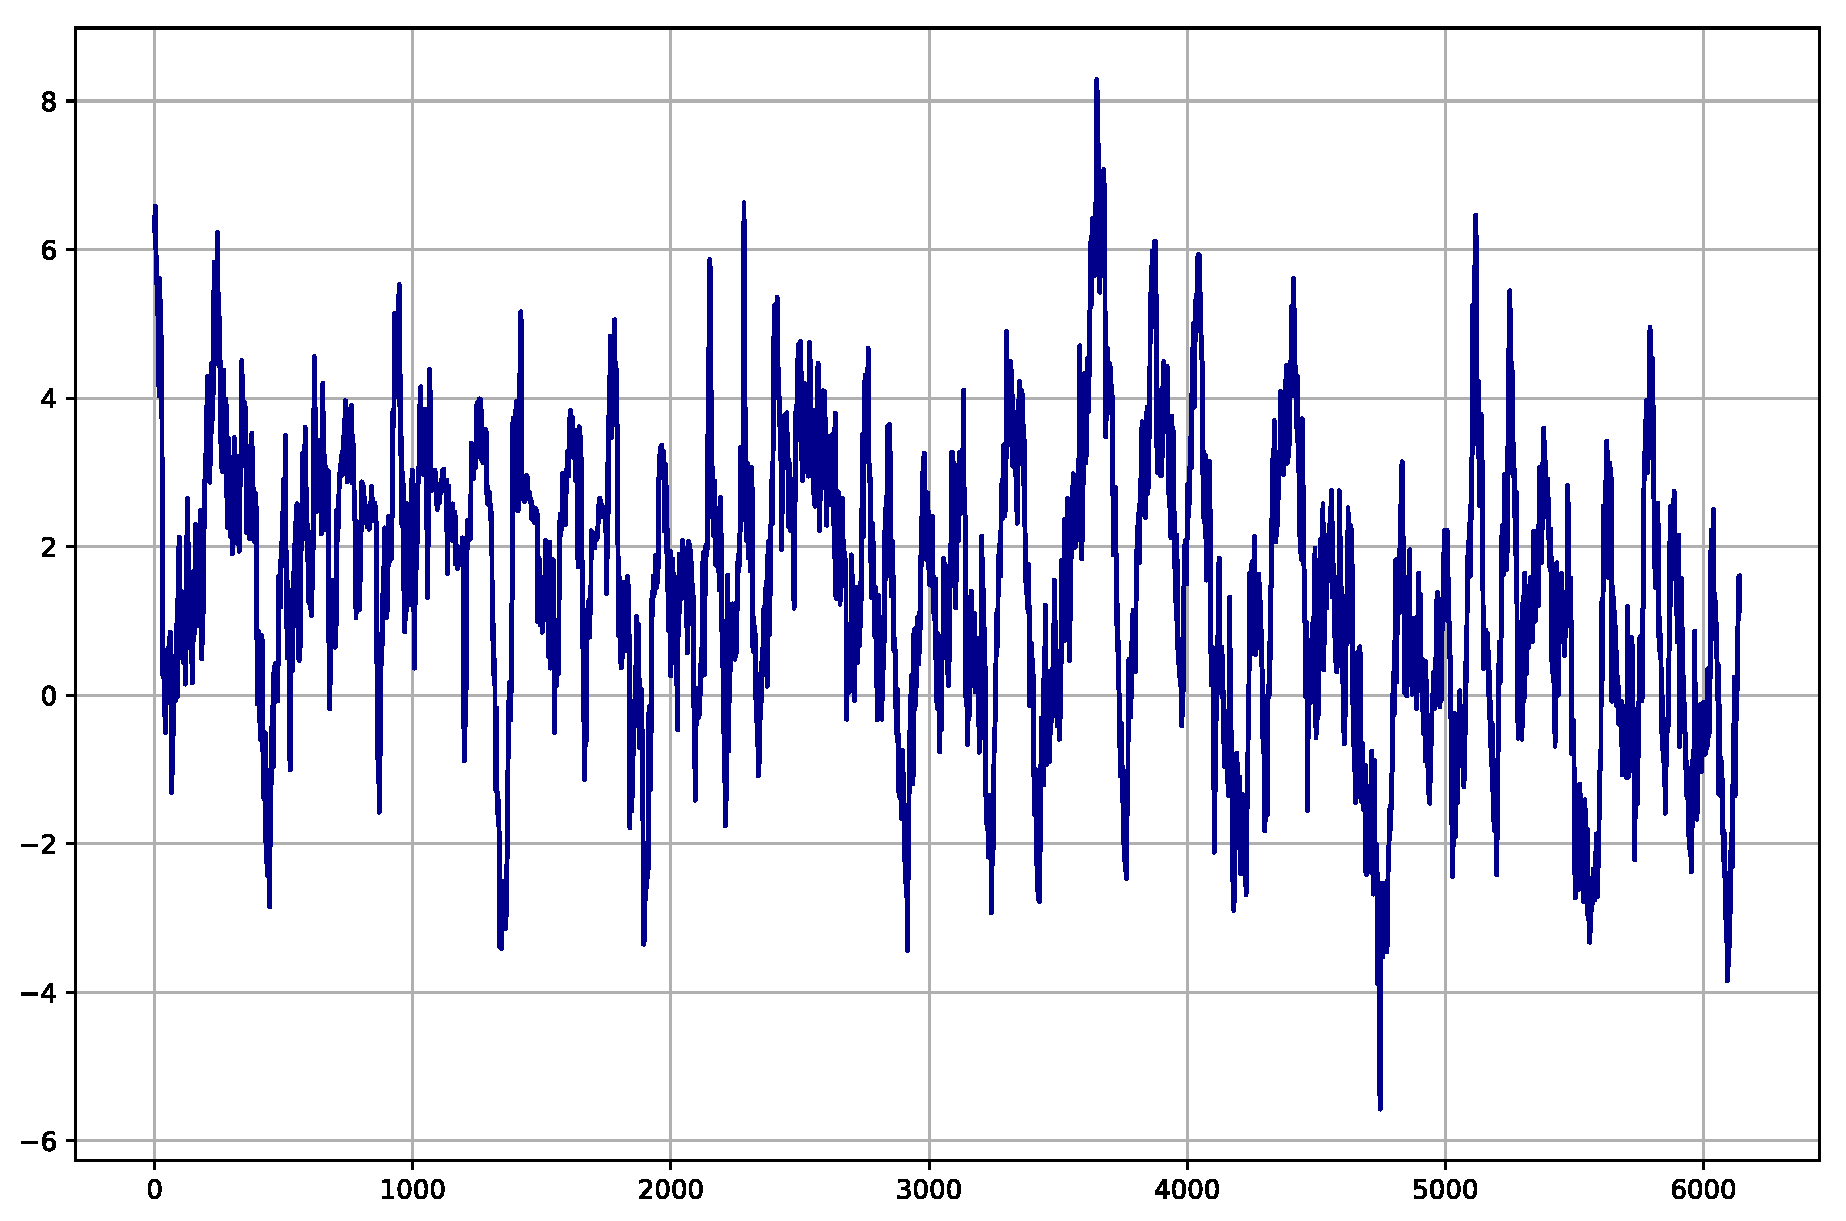
\includegraphics[width=\linewidth]{graphics/sharpe1.pdf}
    \caption{Sharpeov omjer izražen na godišnjoj razini, na prozorima veličine $T = 60$, za simulaciju trgovanja nad podskupom dionica S\&P 500 indeksa.}
    \label{fig:sharpe2}
  \end{figure}

  \begin{sidewaystable}[p]
  \centering
  \captionof{table}{Rezultati testiranja nad S\&P 203 skupu, uz $T = 60, \beta=0$.}
  \label{table:results-1}
  \begin{tabularx}{\hsize}{Xrrrrrrr}
    \toprule
    Parametar: & & & & & & & \\
    \quad a & \multicolumn{3}{c}{0.0} & \multicolumn{3}{c}{0.5} & \multicolumn{1}{c}{1.0} \\ \cmidrule(lr){2-4} \cmidrule(lr){5-7} \cmidrule(lr){8-8}
    \quad b & \multicolumn{1}{c}{0.5} & \multicolumn{1}{c}{1.0} & \multicolumn{1}{c}{2.0} & \multicolumn{1}{c}{0.5} & \multicolumn{1}{c}{1.0} & \multicolumn{1}{c}{2.0} & \multicolumn{1}{c}{/} \\ \midrule
    Prosječni povrat (godišnji) & 0.95339 & 0.88967 & 0.84463 & 0.98336 & 0.95663 & 0.89704 & 1.00223 \\
    Volatilnost (godišnja) & 0.77042 & 0.76595 & 0.74077 & 0.77905 & 0.77054 & 0.76660 & 0.78363 \\
    Sharpeov omjer (godišnji) & 1.23750 & 1.16152 & 1.14020 & 1.26225 & 1.24150 & 1.17015 & 1.27896 \\ \midrule
    Profit: &  &  &  &  &  &  &  \\
    \quad samo pozitivan & 89.27624 & 88.89440 & 88.32548 & 89.58775 & 89.29840 & 89.04414 & 89.55020 \\
    \quad samo negativan & -58.37779 & -59.03715 & -58.41396 & -58.24852 & -58.32385 & -59.02220 & -58.05316 \\
    \quad ukupan & 30.89846 & 29.85725 & 29.91152 & 31.33923 & 30.97456 & 30.02195 & 31.49704 \\
    \quad omjer pozitivnog i negativnog & 1.52928 & 1.50574 & 1.51206 & 1.53803 & 1.53108 & 1.50866 & 1.54256 \\ \midrule
    Prosječna točnost & 0.36485 & 0.39276 & 0.43413 & 0.34902 & 0.36458 & 0.39145 & 0.33241 \\
    Prosječni koeficijent obrtaja & 0.59976 & 0.64224 & 0.73597 & 0.57585 & 0.59947 & 0.64089 & 0.55112 \\ \midrule
    Stvarni profit, uz troškove trgovanja od 0.10\% & 23.46019 & 21.89215 & 20.78402 & 24.19757 & 23.53996 & 22.07361 & 24.66204 \\
    \bottomrule
  \end{tabularx}
\end{sidewaystable}

  \pagebreak

  \section{CROBEX}
  \todo
  Rezultati testiranja nad CROBEX-om \\
  slike i tablica.

  \begin{figure}[p]
    \centering
    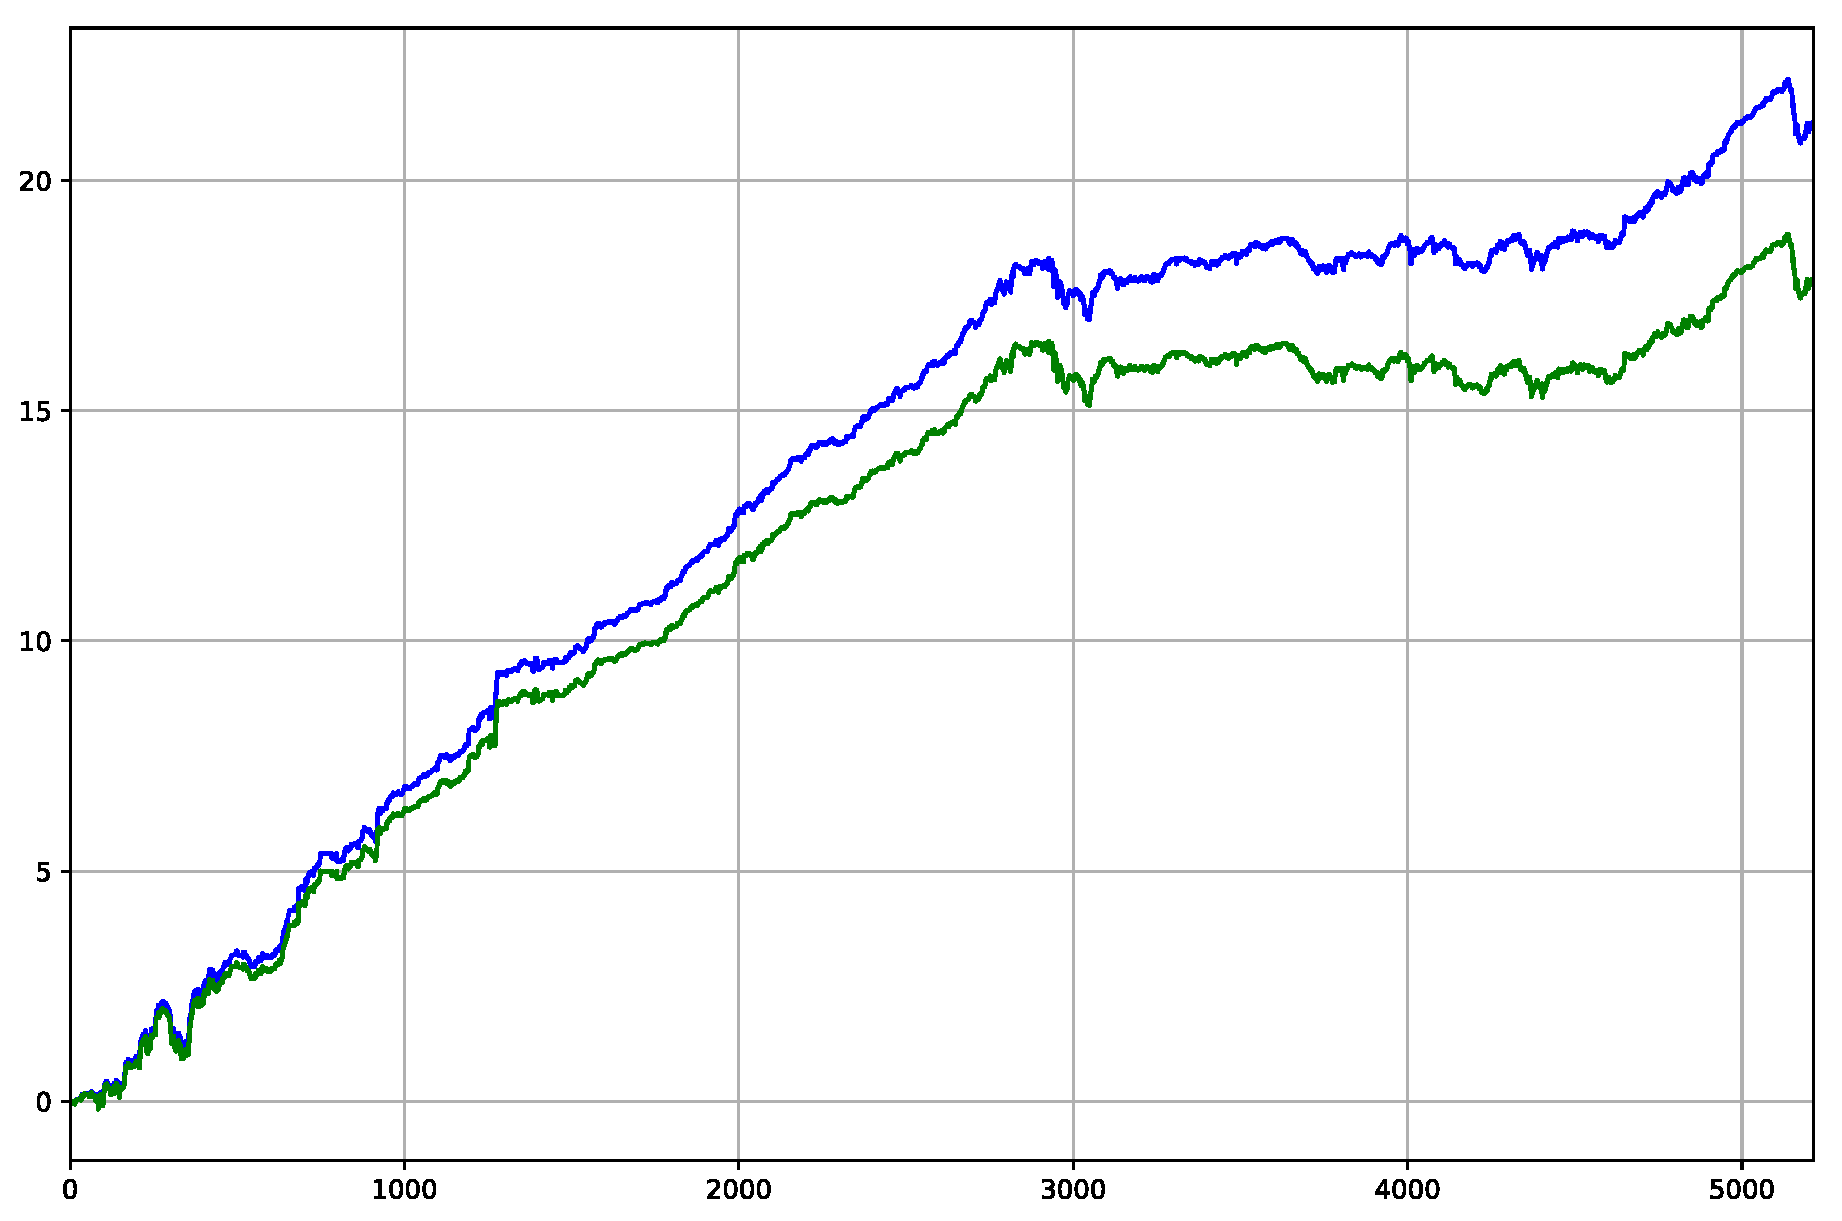
\includegraphics[width=\linewidth]{graphics/results2.pdf}
    \caption{}
    \label{fig:results3}
  \end{figure}
  
  \begin{figure}[p]
    \centering
    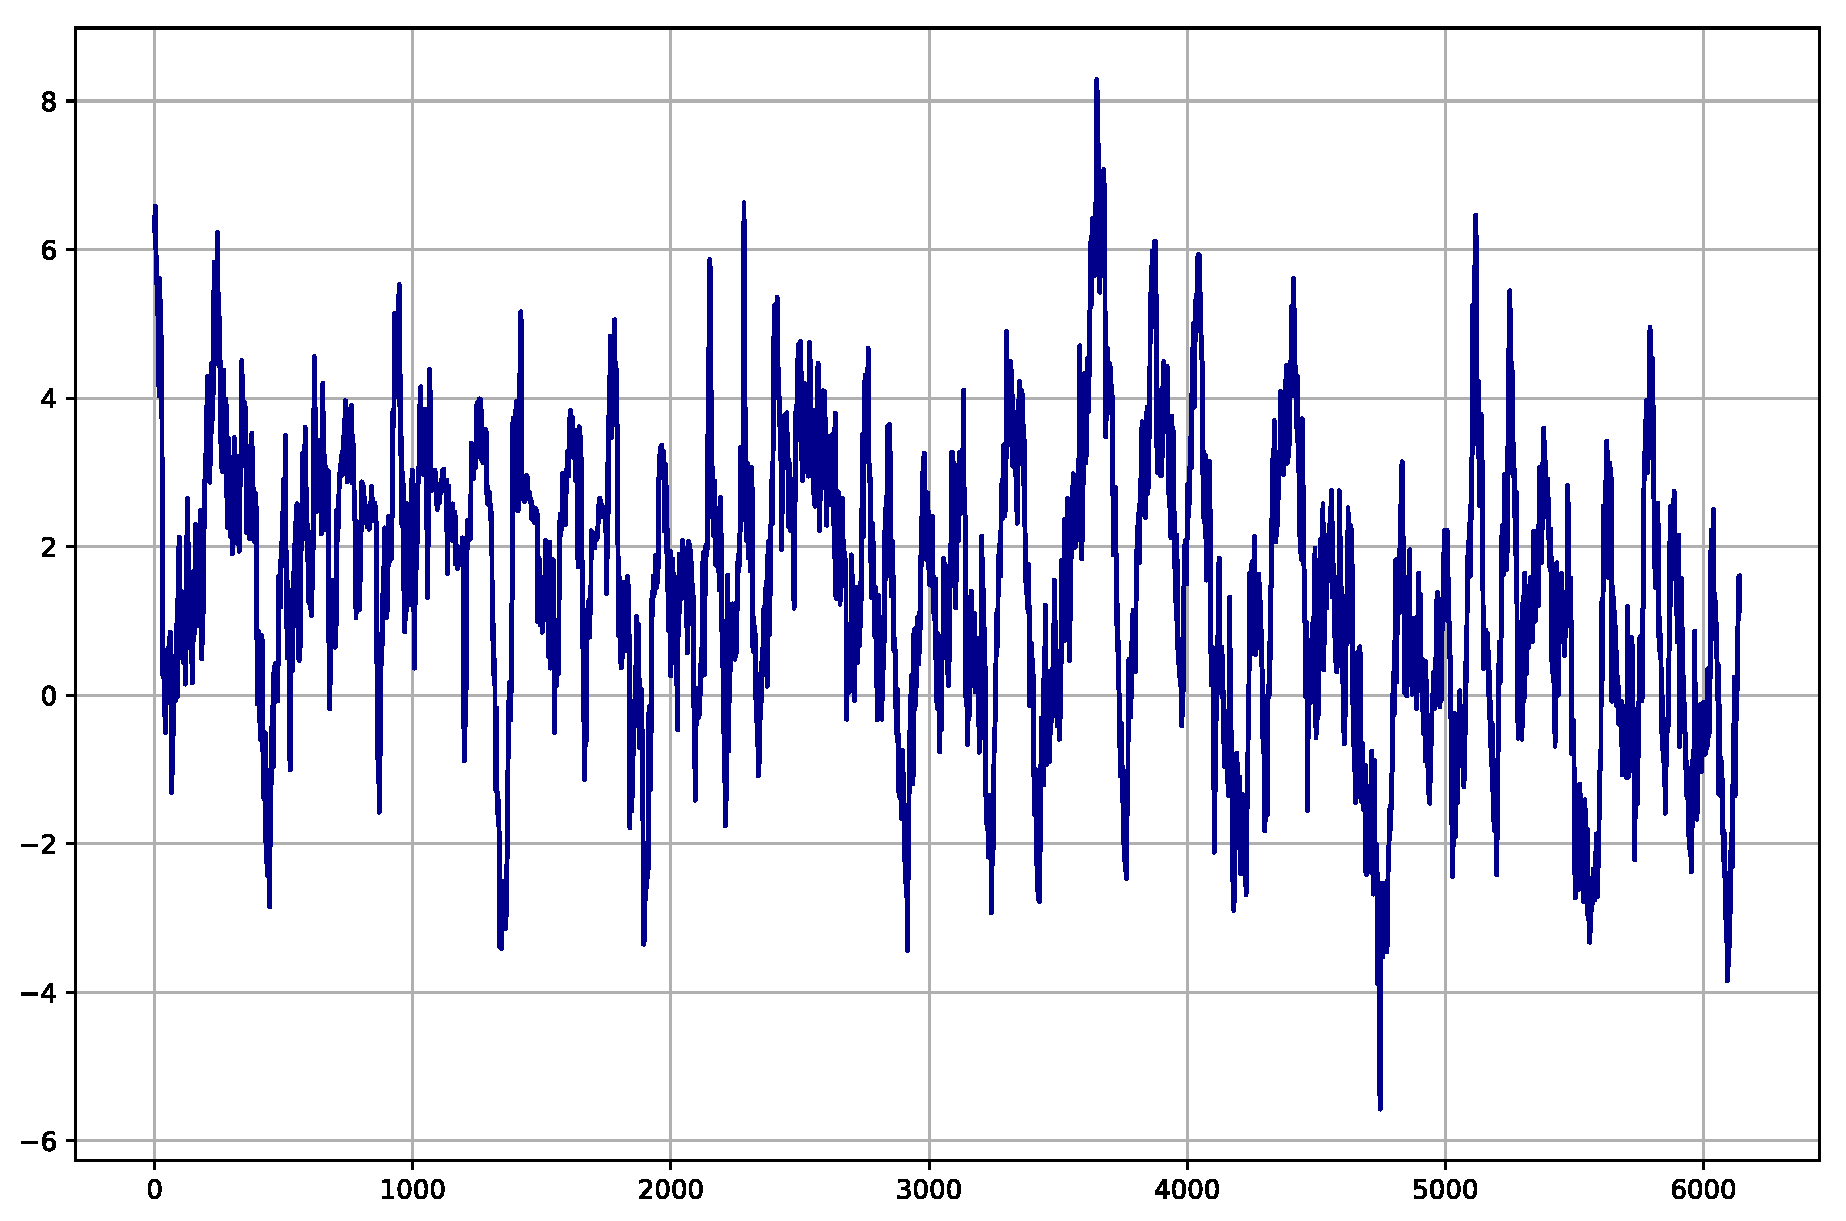
\includegraphics[width=\linewidth]{graphics/sharpe1.pdf}
    \caption{Sharpeov omjer izražen na godišnjoj razini, na prozorima veličine $T = 60$, za simulaciju trgovanja nad podskupom dionica S\&P 500 indeksa.}
    \label{fig:sharpe3}
  \end{figure}
  
  \begin{sidewaystable}[p]
  \centering
  \captionof{table}{Rezultati testiranja nad S\&P 203 skupu, uz $T = 60, \beta=0$.}
  \label{table:results-1}
  \begin{tabularx}{\hsize}{Xrrrrrrr}
    \toprule
    Parametar: & & & & & & & \\
    \quad a & \multicolumn{3}{c}{0.0} & \multicolumn{3}{c}{0.5} & \multicolumn{1}{c}{1.0} \\ \cmidrule(lr){2-4} \cmidrule(lr){5-7} \cmidrule(lr){8-8}
    \quad b & \multicolumn{1}{c}{0.5} & \multicolumn{1}{c}{1.0} & \multicolumn{1}{c}{2.0} & \multicolumn{1}{c}{0.5} & \multicolumn{1}{c}{1.0} & \multicolumn{1}{c}{2.0} & \multicolumn{1}{c}{/} \\ \midrule
    Prosječni povrat (godišnji) & 0.95339 & 0.88967 & 0.84463 & 0.98336 & 0.95663 & 0.89704 & 1.00223 \\
    Volatilnost (godišnja) & 0.77042 & 0.76595 & 0.74077 & 0.77905 & 0.77054 & 0.76660 & 0.78363 \\
    Sharpeov omjer (godišnji) & 1.23750 & 1.16152 & 1.14020 & 1.26225 & 1.24150 & 1.17015 & 1.27896 \\ \midrule
    Profit: &  &  &  &  &  &  &  \\
    \quad samo pozitivan & 89.27624 & 88.89440 & 88.32548 & 89.58775 & 89.29840 & 89.04414 & 89.55020 \\
    \quad samo negativan & -58.37779 & -59.03715 & -58.41396 & -58.24852 & -58.32385 & -59.02220 & -58.05316 \\
    \quad ukupan & 30.89846 & 29.85725 & 29.91152 & 31.33923 & 30.97456 & 30.02195 & 31.49704 \\
    \quad omjer pozitivnog i negativnog & 1.52928 & 1.50574 & 1.51206 & 1.53803 & 1.53108 & 1.50866 & 1.54256 \\ \midrule
    Prosječna točnost & 0.36485 & 0.39276 & 0.43413 & 0.34902 & 0.36458 & 0.39145 & 0.33241 \\
    Prosječni koeficijent obrtaja & 0.59976 & 0.64224 & 0.73597 & 0.57585 & 0.59947 & 0.64089 & 0.55112 \\ \midrule
    Stvarni profit, uz troškove trgovanja od 0.10\% & 23.46019 & 21.89215 & 20.78402 & 24.19757 & 23.53996 & 22.07361 & 24.66204 \\
    \bottomrule
  \end{tabularx}
\end{sidewaystable}

  \pagebreak
  

  \chapter{Zaključak}
  \label{ch:zakljucak}
  Razvijeni algoritam trgovanja temelji se na metodi statističke arbitraže koja radi nad parovima vrijednosnica, i traži takve parove kod kojih se pojavljuju statistički značajna odstupanja, predviđajući pritom da su ona privremena i da će se vratiti u normalno stanje u kratkom periodu.
  Glavni nedostatak metode statističke arbitraže leži u činjenici da ne dolazi do izražaja ukupna interakcija svih raspoloživih vrijednosnica, već se primjećuju samo statistička odstupanja na razini parova.
  To za posljedicu ima jako promjenljiv portfelj i uzrokuje značajne troškove trgovanja, što čini algoritam statističke arbitraže neostvarivim na dugi rok.
  U ovom radu ostvareno je poboljšanje uvođenjem kompleksnih mreža koje omogućuju modeliranje cjelokupne interakcije raspoloživih vrijednosnica, čime je smanjena promjenjljivost portfelja.
  Kao posljedica toga, niži su i troškovi trgovanja te se pokazalo u simulacijama nad povijesnim podacima da je novi algoritam trgovanja ostvariv i donosi dobre rezultate.
  
  U načelu, algoritam radi bolje kada je dostupan veći broj vrijednosnica, i samim time kvadratno veći broj parova vrijednosnica.
  Prilagodba na nekonzistentnost dobivenih preferencija postignuta je u vidu diverzifikacije portfelja proporcionalno nekonzistentnosti.
  Sama mjera nekonzistentnosti služi kao informacija o smislenosti odluka o trgovanju dobivenih algoritmom, te je poželjno da ona bude što veća.
  Unatoč tome, do sada nisu poznate metode za izravnu optimizaciju mjere konzistentnosti, ali su empirijski utvrđene metode za optimizaciju parametara algoritma koje neizravno poboljšavaju performanse algoritma u određenim uvjetima.
  Mogući prostor za napredak ovog algoritma je u korištenju metoda dubokog učenja kojima bi se iz velikih količina podataka o kretanju cijena vrijednosnica mogli naučiti parametri algoritma trgovanja.
%  Algorithm works on pairs of assets, looking for those deviations which are uncommon, so generally it is expected to perform better where there is larger number of assets as more deviations will be discovered.
%  It adapts to the inconsistence of preferences by picking variable number of assets into the portfolio.
  
  \bibliography{literatura}
  \bibliographystyle{babunsrt}

  \appendix
  \chapter{Računanje momenata vremenskog niza na pomičnom prozoru}
  \label{appendix}
  Pri izračunavanju momenata (očekivanje, varijanca) vremenskih nizova nad prozorima konačne duljine, pokazalo se neefikasnim izračunavati svaki prozor zasebno u svakom koraku, jer se većina uzoraka između dva susjedna prozora ponavlja.
  Neka vremenski niz traje ukupno $D$ vremenskih koraka, i neka je veličina vremenskog prozora $T$.
  Momenti se računaju u ukupno $D - T + 1$ vremenskih koraka, svaki put preko prozora veličine $T$, tako da je vremenska složenost nerekurzivne metode računanja momenata $\bigO{\q(D - T + 1\w)\cdot T}$, odnosno približno $\bigO{DT}$, kako je $D \gg T$.
  Stoga se isplati potražiti rekurzivne izraze za očekivanje i varijancu kako bi se izračun mogao obaviti na učinkovitiji način.
  Jedan izvod rekurzivnim izraza dan je u radu \citep{stats}.
  
  Neka je $a\q[t\w]$ vremenski niz, za $t \in \q[0, 1, \ldots, D - 1\w]$.
  Nenormirani momenti $n$-tog reda $S_n$ niza $a\q[t\w]$ nad vremenskim prozorom duljine $T$ definirani su na sljedeći način:
  \begin{equation}
  \label{eq:nonnorm}
  S_n^{(t)} = \sum_{\tau=t-T+1}^{t} a^n\q[\tau\w].
  \end{equation}
  Za nulti moment uvijek vrijedi $S_0^{(t)} = T$ neovisno o $t$.
  Rekurzivni izraz za ažuriranje nenormiranog momenta je očigledan:
  \begin{align}
  S_n^{(t+1)} &= \sum_{\tau=t+1-T+1}^{t+1} a^n\q[\tau\w] \nonumber \\
    &= -a^n\q[t-T+1\w] + \sum_{\tau=t-T+1}^{t} a^n\q[\tau\w] + a^n\q[t+1\w] \nonumber \\
    \label{eq:rec}
    &= -a^n\q[t-T+1\w] + S_n^{(t)} + a^n\q[t+1\w].
  \end{align}
  
  Preko nenormiranih momenata mogu se izraziti očekivanje i varijanca.
  Očekivanje $\Efromto{a\q[\tau\w]}{t - T < \tau \le t}$ je normirani moment prvog reda, i može se izraziti kao:
  \begin{equation}
  \label{eq:recmean}
  \Efromto{a\q[\tau\w]}{t - T < \tau \le t} = \frac{S_1^{(t)}}{S_0^{(t)}},
  \end{equation}
  što je bilo relativno jednostavno za izračunati i bez korištenja nenomiranih momenata.
  No, kod računanja varijance situacija je nešto složenija.
  Varijanca je centrirani i normirani moment drugog reda.
  Prema definiciji, varijanca $\Varfromto{a\q[\tau\w]}{t - T < \tau \le t}$ može se računati još i kao:
  \begin{align}
    \Varfromto{a\q[\tau\w]}{t - T < \tau \le t} &= \Efromto{\q(a\q[\tau\w] - \E{a\q[\tau\w]} \w)^2}{t - T < \tau \le t} \nonumber \\
    &= \Efromto{a^2\q[\tau\w] - 2 a\q[\tau\w] \E{a\q[\tau\w]} + \Esq{a\q[\tau\w]}}{t - T < \tau \le t} \nonumber \\
    &= \Efromto{a^2\q[\tau\w]}{t - T < \tau \le t} \nonumber \\
    & - 2\Esqfromto{a\q[\tau\w]}{t - T < \tau \le t} + \Esqfromto{a\q[\tau\w]}{t - T < \tau \le t} \nonumber \\
    \label{eq:varalt}
    &= \Efromto{a^2\q[\tau\w]}{t - T < \tau \le t} - \Esqfromto{a\q[\tau\w]}{t - T < \tau \le t}
  \end{align}
  Izraz $\Efromto{a^2\q[\tau\w]}{t - T < \tau \le t}$ u (\ref{eq:varalt}) može se preko nenormiranih momenata izraziti kao $\q. S_2^{(t)} \middle/ S_0^{(t)} \w.$,
  a izraz $\Esqfromto{a\q[\tau\w]}{t - T < \tau \le t}$ kao $\q. \q(S_1^{(t)}\w)^2 \middle/ \q(S_0^{(t)}\w)^2 \w.$.
  Konačno, varijanca se može izraziti preko nenormiranih momenata kao:
  \begin{equation}
    \label{eq:recvar}
    \Varfromto{a\q[\tau\w]}{t - T < \tau \le t} = \frac{S_2^{(t)}}{S_0^{(t)}} - \frac{\q(S_1^{(t)}\w)^2}{\q(S_0^{(t)}\w)^2}
    = \frac{S_0^{(t)} S_2^{(t)} - \q(S_1^{(t)}\w)^2}{\q(S_0^{(t)}\w)^2}.
  \end{equation}
  
  Na ovaj način moguće je izračunati očekivanje i varijancu nad pomičnim prozorom na mnogo učinkovitiji način nego nerekurzivnim postupkom.
  U početku je potrebno izračunati momente $S_0^{(T - 1)}$, $S_1^{(T - 1)} $ i $S_2^{(T - 1)}$ prema (\ref{eq:nonnorm}), te iz njih $\Efromto{a\q[\tau\w]}{0 \le \tau < T}$ i $\Varfromto{a\q[\tau\w]}{0 \le \tau < T}$ prema (\ref{eq:recmean}) i (\ref{eq:recvar}); u složenosti $\bigO{T}$.
  Nadalje, za svaki sljedeći pomak vremenskog prozora rekurzivno se ažuriraju vrijednosti nenormiranih momenata koristeći (\ref{eq:rec}), te se putem njih izračunavaju očekivanje i varijanca ponovno koristeći (\ref{eq:recmean}) i (\ref{eq:recvar}), u složenosti $\bigO{T - D}$.
  Time je ukupna vremenska složenost algoritma pala s $\bigO{DT}$ na $\bigO{D}$.

  \begin{sazetak}
  U ovom radu istražene su metode za analizu financijskih vremenskih nizova, temeljene na algoritmu statističke arbitraže.
  Rezultati istraživanja zaokruženi su u samostalan algoritam za simulaciju trgovanja vrijednosnicama temeljenu na povijesnim podacima, i trgovanje vrijednosnicama nad podacima koji dolaze u stvarnom vremenu.
  Ulazne podatke za algoritam čini kretanje cijena nekog broja vrijednosnica u nekom razdoblju.
  Na temelju njih, konstruira se kompleksna mreža koja opisuje odnos vrijednosnica u svakom vremenskom koraku.
  Iz dobivene mreže procjenjuje se poredak vrijednosnica po preferenciji i računa se pouzdanost same procjene poretka.
  Konačno, na temelju poretka i pouzdanosti njegove procjene konstruira se portfelj koji čine vrijednosnice s najvećom preferencijom.
  Algoritam je simuliran nad stvarnim povijesnim podacima i polučio je uspješne rezultate.
  Iako su istraženi specijalno financijski vremenski nizovi, korišteni matematički i statistički postupci koji su korišteni lako mogu poslužiti i u druge svrhe.

  \kljucnerijeci{vremenski nizovi, financije, statistička arbitraža, relacija preferencije, graf toka preferencija, metoda potencijala.}
  \end{sazetak}
  \pagebreak

  \engtitle{Complex network based time series analysis}
  \begin{abstract}
  In this thesis, methods for financial time series analysis using statistical arbitrage algorithm are researched.
  Results of the research are summed up into standalone algorithm for simulation of assets trading based on historical data, and also for real world assets trading on live data.
  Input data for the algorithm are prices of some number of assets during some time span.
  Next, a complex network is constructed using the input data that describes relations among the assets at the each time step.
  Then, the ranking based on preference of assets is derived from the network and also the confidence of derived ranking is obtained.
  Finally, portfolio is constructed from the most preferred assets, by using ranking and its confidence.
  Simulating the algorithm on the real historical data has yielded significant results.
  Although the research in this thesis has been done on financial time series, mathematical and statistical methods used can easily prove useful in other applications.

  \keywords{time series, finances, statistical arbitrage, preference relation, preference flow graph, potential method.}
  \end{abstract}

\end{document}
